\documentclass{article}
\usepackage{etoolbox}       %

\usepackage{graphicx}  %

\usepackage[parfill]{parskip}
\usepackage{amsmath,amsthm}
\usepackage{mathtools}  %
\usepackage[dvipsnames]{xcolor}         %

\newtoggle{arxiv}
\toggletrue{arxiv}

  \usepackage[parfill]{parskip}
  \usepackage[citestyle=authoryear-comp,sorting=nyt,maxbibnames=99,backend=biber]{biblatex}
  \newcommand{\citep}{\parencite}
  \newcommand{\citet}{\textcite}
  \addbibresource{biblio.bib}  %

  \setlength{\textwidth}{6.8in}  %
  \setlength{\textheight}{9in}
  \setlength{\oddsidemargin}{0in}
  \setlength{\evensidemargin}{0in}
  \setlength{\topmargin}{-0.5in}
  \newlength{\defbaselineskip}
  \setlength{\defbaselineskip}{\baselineskip}
  \setlength{\marginparwidth}{0.8in}
  \setlength{\parskip}{6pt}%
  \setlength{\parindent}{0pt}%

  \RequirePackage[T1]{fontenc}
  \RequirePackage[tt=false, type1=true]{libertine}
  \RequirePackage[varqu]{zi4}
  \RequirePackage[libertine]{newtxmath}


\usepackage{bm}

\usepackage[inline]{enumitem}
\usepackage{booktabs}
\usepackage[dvipsnames]{xcolor}  %
\usepackage{subcaption}
\usepackage{multirow}
\usepackage{wrapfig}
\usepackage{algorithm,algorithmicx,algpseudocode}
\usepackage{nicematrix}


\usepackage[frozencache,cachedir=.]{minted} %
% \usepackage[finalizecache,cachedir=.]{minted} %

\usepackage[colorlinks=true,linkcolor=blue,citecolor=magenta,urlcolor=red]{hyperref}
\usepackage[capitalise,noabbrev]{cleveref}


\usepackage{import}


\newtheorem{theorem}{Theorem}[section]  %
\newtheorem{corollary}[theorem]{Corollary}  %

\newtheorem{lemma}[theorem]{Lemma}
\newtheorem{proposition}[theorem]{Proposition}
\newtheorem{definition}[theorem]{Definition}
\newtheorem{conjecture}[theorem]{Conjecture}
\newtheorem{remark}{Remark}

\usepackage{pifont}%
\newcommand{\cmark}{\ding{51}}%
\newcommand{\xmark}{\ding{55}}%

\DeclarePairedDelimiter\parens{\lparen}{\rparen}
\DeclarePairedDelimiter\abs{\lvert}{\rvert}
\DeclarePairedDelimiter\norm{\lVert}{\rVert}
\DeclarePairedDelimiter\floor{\lfloor}{\rfloor}
\DeclarePairedDelimiter\ceil{\lceil}{\rceil}
\DeclarePairedDelimiter\braces{\lbrace}{\rbrace}
\DeclarePairedDelimiter\bracks{\lbrack}{\rbrack}
\DeclarePairedDelimiter\angles{\langle}{\rangle}


\DeclareMathOperator{\ssm}{\mathsf{SSM}}
\DeclareMathOperator{\lassm}{\mathsf{LASSM}}
\DeclareMathOperator{\cumsum}{\mathsf{cumsum}}


\newcommand{\R}{\mathbb{R}}
\newcommand{\dt}{\Delta}
\newcommand{\A}{\bm{A}}
\newcommand{\B}{\bm{B}}
\newcommand{\C}{\bm{C}}
\newcommand{\D}{\bm{D}}
\newcommand{\K}{\overline{\bm{K}}}
\newcommand{\dA}{\overline{\bm{A}}}
\newcommand{\dB}{\overline{\bm{B}}}

\newcommand{\AB}{(\A, \B)}
\newcommand{\ABC}{(\A, \B, \C)}
\newcommand{\dtAB}{(\dt, \A, \B)}
\newcommand{\dtABC}{(\dt, \A, \B, \C)}
\newcommand{\dAB}{(\dA, \dB)}

\newcommand{\para}[1]{\iftoggle{arxiv}{\paragraph{#1}}{\textbf{#1}}}
\newcommand{\maybe}[1]{\textcolor{blue}{#1}}

\newcommand*\samethanks[1][\value{footnote}]{\footnotemark[#1]}


  \title{Transformers are SSMs: Generalized Models and Efficient Algorithms \\ Through Structured State Space Duality}
  \usepackage{authblk}
  \author[$^1$]{Tri Dao\thanks{Alphabetical by last name.}}
  \author[$^2$]{Albert Gu\samethanks}
  \affil[$^1$]{Department of Computer Science, Princeton University}
  \affil[$^2$]{Machine Learning Department, Carnegie Mellon University}
  \affil[ ]{{\texttt{tri@tridao.me}}, {\texttt{agu@cs.cmu.edu}}}
  \date{}

\begin{document}

  \maketitle


Scaling Transformers to longer sequence lengths has been a major problem in the
last several years, promising to improve performance in language modeling and
high-resolution image understanding, as well as to unlock new applications in
code, audio, and video generation.
The attention layer is the main bottleneck in scaling to longer sequences, as
its runtime and memory increase quadratically in the sequence length.
\sysnameone~\citep{dao2022flashattention} exploits the asymmetric GPU memory
hierarchy to bring significant memory saving (linear instead of quadratic) and
runtime speedup (2-4$\times$ compared to optimized baselines), with no approximation.
However, \sysnameone is still not nearly as fast as optimized matrix-multiply
(GEMM) operations, reaching only 25-40\% of the theoretical maximum FLOPs/s.
We observe that the inefficiency is due to suboptimal work partitioning between
different thread blocks and warps on the GPU, causing either low-occupancy or
unnecessary shared memory reads/writes.
We propose \sysname, with better work partitioning to address these issues.
In particular, we (1) tweak the algorithm to reduce the number of non-matmul
FLOPs (2) parallelize the attention computation, even for a single head, across
different thread blocks to increase occupancy, and (3) within each thread block,
distribute the work between warps to reduce communication through shared memory.
These yield around 2$\times$ speedup compared to \sysnameone, reaching 50-73\% of the
theoretical maximum FLOPs/s on A100 and getting close to the efficiency of GEMM
operations.
We empirically validate that when used end-to-end to train GPT-style models,
\sysname reaches training speed of up to 225 TFLOPs/s per A100 GPU (72\% model
FLOPs utilization).\footnote{\sysname
  is available at \url{https://github.com/Dao-AILab/flash-attention}}

% models with up to 2$\times$ longer sequence length compared to \sysnameone, in the
% same amount of time, leading to better downstream performance.\footnote{\sysname
%   is available at \url{https://github.com/Dao-AILab/flash-attention}}

\documentclass[11pt]{report}
\usepackage[margin=2cm]{geometry}
\usepackage{graphicx}
\usepackage{float}
\usepackage{times}
\usepackage{url}
\usepackage[dvipsnames]{xcolor}
\usepackage{hyperref}

\newcommand{\specialcell}[2][c]{\begin{tabular}[#1]{@{}c@{}}#2\end{tabular}}

\newcommand{\Gap}{\texorpdfstring{\hfill}{}}
\newcommand{\Rec}{\texorpdfstring{{\small\emph{\color{ccai-blue}{\fbox{High Leverage}}}}}{}}
\newcommand{\HighRisk}{\texorpdfstring{{\small\emph{\color{ccai-yellow-darker}{\fbox{Uncertain Impact}}}}}{}}
\newcommand{\Longterm}{\texorpdfstring{{\small\emph{\color{ccai-green}{\fbox{Long-term}}}}}{}}

\begin{document}

\begin{abstract}
Climate change is one of the greatest challenges facing humanity, and we, as machine learning experts, may wonder how we can help. Here we describe how machine learning can be a powerful tool in reducing greenhouse gas emissions and helping society adapt to a changing climate. From smart grids to disaster management, we identify high impact problems where existing gaps can be filled by machine learning, in collaboration with other fields. Our recommendations encompass exciting research questions as well as promising business opportunities. We call on the machine learning community to join the global effort against climate change.
\vskip .5in
\end{abstract}

\part*{Introduction}
The effects of climate change are increasingly visible.\footnote{For a layman's introduction to the topic of climate change, see \cite{romm2018climate, archer2010climate}.} Storms, droughts, fires, and flooding have become stronger and more frequent \cite{field2012managing}. Global ecosystems are changing, including the natural resources and agriculture on which humanity depends. The 2018 intergovernmental report on climate change estimated that the world will face catastrophic consequences unless global greenhouse gas emissions are eliminated within thirty years \cite{ipcc_global_2018}. Yet year after year, these emissions rise.

Addressing climate change involves mitigation (reducing emissions) and adaptation (preparing for unavoidable consequences). Both are multifaceted issues. Mitigation of greenhouse gas (GHG) emissions requires changes to electricity systems, transportation, buildings, industry, and land use. Adaptation requires planning for resilience and disaster management, given an understanding of climate and extreme events. Such a diversity of problems can be seen as an opportunity: there are many ways to have an impact.

In recent years, machine learning (ML) has been recognized as a broadly powerful tool for technological progress. Despite the growth of movements applying ML and AI to problems of societal and global good,\footnote{See the AI for social good movement (e.g.~\cite{hager2019artificial, berendt2019ai}), ML for the developing world~\cite{de2018machine}, the computational sustainability movement (e.g.~\cite{kelling2018computational, joppa2017case, lassig2016computational, gomes2009computational, dietterich2009machine}, the American Meteorological Society's Committee on AI Applications to Environmental Science, and the field of Climate Informatics (\url{www.climateinformatics.org}) \cite{Monteleoni2013chapter}, as well as the relevant survey papers \cite{faghmous2014big, kaack2019challenges, ford2016opinion}.} there remains the need for a concerted effort to identify how these tools may best be applied to tackle climate change. Many ML practitioners wish to act, but are uncertain how. On the other side, many fields have begun actively seeking input from the ML community.

This paper aims to provide an overview of where machine learning can be applied with high impact in the fight against climate change, through either effective engineering or innovative research. The strategies we highlight include climate mitigation and adaptation, as well as meta-level tools that enable other strategies. In order to maximize the relevance of our recommendations, we have consulted experts across many fields (see \hyperref[sec:acknowledgments]{{\small{Acknowledgments}}}) in the preparation of this paper.


\begin{table}
\begin{small}
\begin{center}
\begin{tabular}{l l l l l l l l l l l l}  \toprule
     \multicolumn{2}{l}{ }
         & \small{\rotatebox{90}{\parbox{2.2cm}{Causal\\inference}}}
         & \small{\rotatebox{90}{\parbox{2.2cm}{Computer\\vision}}}
         & \small{\rotatebox{90}{\parbox{2.2cm}{Interpretable\\models}}}
         & \small{\rotatebox{90}{NLP}}
         & \small{\rotatebox{90}{\parbox{2.2cm}{RL \& Control}}}
        %  & \small{\rotatebox{90}{Robotics}}
         & \small{\rotatebox{90}{\parbox{2.2cm}{Time-series analysis}}}
         & \small{\rotatebox{90}{\parbox{2.2cm}{Transfer\\learning}}}
         & \small{\rotatebox{90}{\parbox{2.2cm}{Uncertainty\\quantification}}}
         & \small{\rotatebox{90}{\parbox{2.2cm}{Unsupervised\\learning}}}
    \\ \midrule
    \rowcolor{ccai-blue-lightest}
    \multicolumn{2}{l}{1 \hyperref[sec:electricity-systems]{Electricity systems}} 
        & % Causal inf
        &  % Comp vision
        & % Interpretable ml
        & % nlp
        & % rl + control
        & % time series
        & % transfer
        & % UQ
        & \\% unsupervised \ref{sub
    & \hyperref[sec:electricity-lowCarbon]{Enabling low-carbon electricity}
        & % Causal inf
        & $\bullet$% Comp vision
        & $\bullet$% % Interpretable ml
        & % % nlp
        & $\bullet$%% rl + control
        & $\bullet$% % time series
        & % transfer
        & $\bullet$% % UQ
        & $\bullet$\\% unsupervised 
    & \hyperref[sec:electricity-currentSystemImpact]{Reducing current-system impacts}
        & % Causal inf
        & $\bullet$% Comp vision
        & % Interpretable ml
        & % nlp
        & % rl + control
        & $\bullet$% % time series
        & % transfer
        & $\bullet$% % UQ
        & $\bullet$\\% unsupervised 
    & \hyperref[sec:electricity-developing]{Ensuring global impact}
        & % Causal inf
        & $\bullet$% Comp vision
        & % Interpretable ml
        & % nlp
        & % rl + control
        & % time series
        & $\bullet$ % transfer
        & % UQ
        & $\bullet$\\% unsupervised 
    \rowcolor{ccai-blue-lightest}
    \multicolumn{2}{l}{2 \hyperref[sec:transportation]{Transportation}} 
        & % Causal inf
        & % Comp vision
        &% Interpretable ml
        & % nlp
        & % rl + control
        & % time series
        & % transfer
        & % UQ
        & \\% unsupervised 
    & \hyperref[sec:TReducing]{Reducing transport activity}
        & % Causal inf
        & $\bullet$% Comp vision
        & % Interpretable ml
        & % nlp
        & % rl + control
        & $\bullet$% time series
        & % transfer
        & $\bullet$% UQ
        & $\bullet$\\% unsupervised     
   & \hyperref[sec:TEfficient]{Improving vehicle efficiency}
        & % Causal inf
        & $\bullet$% Comp vision
        & % Interpretable ml
        & % nlp
        & $\bullet$% rl + control
        & % time series
        & % transfer
        & % UQ
        & \\% unsupervised    
   & \hyperref[sec:TFuels]{Alternative fuels \& electrification}
        & % Causal inf
        & % Comp vision
        & % Interpretable ml
        & % nlp
        & $\bullet$% rl + control
        & % time series
        & % transfer
        & % UQ
        & $\bullet$ \\% unsupervised    
   & \hyperref[sec:modalshift]{Modal shift}
        & $\bullet$% Causal inf
        & $\bullet$% Comp vision
        & % Interpretable ml
        & % nlp
        & % rl + control
        & $\bullet$% time series
        & % transfer
        & $\bullet$% UQ
        & \\% unsupervised    
    \rowcolor{ccai-blue-lightest}
    \multicolumn{2}{l}{3 \hyperref[sec:buildings-cities]{Buildings and cities}} 
        & % Causal inf
        & % Comp vision
        & % Interpretable ml
        & % nlp
        & % rl + control
        & % time series
        & % transfer
        & % UQ
        & \\% unsupervised 
    & \hyperref[sec:indv]{Optimizing buildings}
        & $\bullet$% Causal inf
        & % Comp vision
        & % Interpretable ml
        & % nlp
        & $\bullet$% rl + control
        & $\bullet$% time series
        & $\bullet$% transfer
        & % UQ
        & \\% unsupervised 
    & \hyperref[sec:distr]{Urban planning}
        & % Causal inf
        & $\bullet$% Comp vision
        & % Interpretable ml
        & % nlp
        & % rl + control
        & $\bullet$% time series
        & $\bullet$% transfer
        & % UQ
        & $\bullet$\\% unsupervised 
    & \hyperref[sec:cities]{The future of cities}
        & % Causal inf
        & % Comp vision
        & % Interpretable ml
        & $\bullet$%% nlp
        & % rl + control
        & %% time series
        & $\bullet$%% transfer
        & $\bullet$% UQ
        & $\bullet$\\% unsupervised 
    \rowcolor{ccai-blue-lightest}
    \multicolumn{2}{l}{4 \hyperref[sec:industry]{Industry}} 
        & % Causal inf
        & % Comp vision
        & % Interpretable ml
        & % nlp
        & % rl + control
        & % time series
        & % transfer
        & % UQ
        & \\% unsupervised 
    & \hyperref[sec:supplychains]{Optimizing supply chains}
        & % Causal inf
        & $\bullet$ %% Comp vision
        & % Interpretable ml
        & % nlp
        & $\bullet$ % rl + control
        & $\bullet$ % time series
        & % transfer
        & % UQ
        & \\% unsupervised 
    & \hyperref[sec:materialsandconstruction]{Improving materials}
        & %% Causal inf
        & % Comp vision
        & % Interpretable ml
        & % nlp
        & % rl + control
        & % time series
        & %% transfer
        & % UQ
        & $\bullet$ \\% unsupervised 
    & \hyperref[sec:demandresponse]{Production \& energy}
        & %% Causal inf
        & $\bullet$%% Comp vision
        & $\bullet$ %% Interpretable ml
        & % nlp
        & $\bullet$% rl + control
        & %% time series
        & %% transfer
        & % UQ
        & \\% unsupervised 
    \rowcolor{ccai-blue-lightest}
    \multicolumn{2}{l}{5 \hyperref[sec:afolu]{Farms \& forests}} 
        & % Causal inf
        & % Comp vision
        & % Interpretable ml
        & % nlp
        & % rl + control
        & % time series
        & % transfer
        & % UQ
        & \\% unsupervised 
    & \hyperref[sec:emissions-detection]{Remote sensing of emissions}
        & % Causal inf
        & $\bullet$% Comp vision
        & % Interpretable ml
        & % nlp
        & % rl + control
        & % time series
        & % transfer
        & % UQ
        & \\% unsupervised 
    & \hyperref[sec:agriculture]{Precision agriculture}
        & % Causal inf
        & $\bullet$% Comp vision
        & % Interpretable ml
        & % nlp
        & $\bullet$% rl + control
        & $\bullet$% time series
        & % transfer
        & % UQ
        & \\% unsupervised 
    & \hyperref[sec:peatlands]{Monitoring peatlands}
        & % Causal inf
        & $\bullet$% Comp vision
        & % Interpretable ml
        & % nlp
        & % rl + control
        & % time series
        & % transfer
        & % UQ
        & \\% unsupervised 
    & \hyperref[sec:forests]{Managing forests}
        & % Causal inf
        & $\bullet$% Comp vision
        & % Interpretable ml
        & % nlp
        & $\bullet$ % rl + control
        & $\bullet$ % time series
        & % transfer
        & % UQ
        & \\% unsupervised 
    \rowcolor{ccai-blue-lightest}
    \multicolumn{2}{l}{6 \hyperref[sec:ccs]{Carbon dioxide removal}}
        & % Causal inf
        & % Comp vision
        & % Interpretable ml
        & % nlp
        & % rl + control
        & % time series
        & % transfer
        & % UQ
        & \\
    & \hyperref[sec:ccs]{Direct air capture}
        & % Causal inf
        & % Comp vision
        & % Interpretable ml
        & % nlp
        & % rl + control
        & % time series
        & % transfer
        & % UQ
        & $\bullet$\\% unsupervised 
    & \hyperref[subsubsec: sequestrativervin]{Sequestering~\cd}
        & % Causal inf
        & $\bullet$% Comp vision
        & % Interpretable ml
        & % nlp
        & % rl + control
        & % time series
        & % transfer
        & $\bullet$% UQ
        & $\bullet$\\% unsupervised 
    \rowcolor{ccai-blue-lightest}
    \multicolumn{2}{l}{7 \hyperref[sec: climate prediction]{Climate prediction}} 
        & % Causal inf
        & % Comp vision
        & % Interpretable ml
        & % nlp
        & % rl + control
        & % time series
        & % transfer
        & % UQ
        & \\% unsupervised 
    & \hyperref[sec:climate-models-params]{Uniting data, ML \& climate science}
        & % Causal inf
        & $\bullet$% Comp vision
        & $\bullet$% Interpretable ml
        & % nlp
        & % rl + control
        & $\bullet$% time series
        & % transfer
        & $\bullet$% UQ
        & \\% unsupervised 
    & \hyperref[sec:models-extreme-events]{Forecasting extreme events}
        & % Causal inf
        & $\bullet$% Comp vision
        & $\bullet$% Interpretable ml
        & % nlp
        & % rl + control
        & $\bullet$% time series
        & % transfer
        & $\bullet$% UQ
        & \\% unsupervised 
    \rowcolor{ccai-blue-lightest}
    \multicolumn{2}{l}{8 \hyperref[sec:societal-impacts]{Societal impacts}} 
        & % Causal inf
        & % Comp vision
        & % Interpretable ml
        & % nlp
        & % rl + control
        & % time series
        & % transfer
        & % UQ
        & \\% unsupervised 
    & \hyperref[subsub:ecology]{Ecology}
        & % Causal inf
        & $\bullet$% Comp vision
        & % Interpretable ml
        & % nlp
        & % rl + control
        & % time series
        & $\bullet$% transfer
        & % UQ
        & \\% unsupervised 
    & \hyperref[subsub:infrastructure]{Infrastructure}
        & % Causal inf
        & % Comp vision
        & % Interpretable ml
        & % nlp
        & $\bullet$% rl + control
        & $\bullet$% time series
        & % transfer
        & $\bullet$% UQ
        & \\% unsupervised 
    & \hyperref[subsub:social_systems]{Social systems}
        & % Causal inf
        & $\bullet$% Comp vision
        & % Interpretable ml
        & % nlp
        & % rl + control
        & $\bullet$% time series
        & % transfer
        & % UQ
        & $\bullet$\\% unsupervised 
    & \hyperref[subsub:crisis]{Crisis}
        & % Causal inf
        & $\bullet$% Comp vision
        & % Interpretable ml
        & $\bullet$% nlp
        & % rl + control
        & % time series
        & % transfer
        & % UQ
        & \\% unsupervised 
    \rowcolor{ccai-blue-lightest}
    \multicolumn{2}{l}{9 \hyperref[sec:geoengineering]{Solar geoengineering}} 
        & % Causal inf
        & % Comp vision
        & % Interpretable ml
        & % nlp
        & % rl + control
        & % time series
        & % transfer
        & % UQ
        & \\% unsupervised 
    & \hyperref[subsub:better-aerosols]{Understanding \& improving aerosols}
        & % Causal inf
        & % Comp vision
        & % Interpretable ml
        & % nlp
        & % rl + control
        & $\bullet$% time series
        & % transfer
        & $\bullet$% UQ
        & \\% unsupervised 
    & \hyperref[subsub:planetary-control]{Engineering a planetary control system}
        & % Causal inf
        & % Comp vision
        & % Interpretable ml
        & % nlp
        & $\bullet$% rl + control
        & % time series
        & % transfer
        & $\bullet$% UQ
        & \\% unsupervised 
    & \hyperref[subsub:impact-models]{Modeling impacts}
        & % Causal inf
        & % Comp vision
        & % Interpretable ml
        & % nlp
        & % rl + control
        & $\bullet$% time series
        & % transfer
        & $\bullet$% UQ
        & \\% unsupervised 
    \rowcolor{ccai-blue-lightest}
    \multicolumn{2}{l}{10 \hyperref[sec:tools-individuals]{Individual action}} 
        & % Causal inf
        & % Comp vision
        & % Interpretable ml
        & % nlp
        & % rl + control
        & % time series
        & % transfer
        & % UQ
        & \\% unsupervised 
    & \hyperref[sec:personal_carbon_footprint]{Understanding personal footprint}
        & $\bullet$% Causal inf
        & % Comp vision
        & % Interpretable ml
        & $\bullet$% nlp
        & $\bullet$% rl + control
        & $\bullet$% time series
        & % transfer
        & % UQ
        & \\% unsupervised 
    & \hyperref[sec:behavior_change]{Facilitating behavior change}
        & % Causal inf
        & % Comp vision
        & % Interpretable ml
        & $\bullet$% nlp
        & % rl + control
        & % time series
        & % transfer
        & % UQ
        & $\bullet$\\% unsupervised 
    \rowcolor{ccai-blue-lightest}
    \multicolumn{2}{l}{11 \hyperref[sec:toolsforsociety]{Collective decisions}} 
        & % Causal inf
        & % Comp vision
        & % Interpretable ml
        & % nlp
        & % rl + control
        & % time series
        & % transfer
        & % UQ
        &  \\% unsupervised 
    & \hyperref[sec:coordination]{Modeling social interactions}
        & % Causal inf
        & % Comp vision
        & $\bullet$ % Interpretable ml
        & % nlp
        & $\bullet$ % rl + control
        & % time series
        & % transfer
        & % UQ
        & \\% unsupervised 
    & \hyperref[sec:decisionmaking]{Informing policy}
        & $\bullet$ % Causal inf
        & $\bullet$ % Comp vision
        & % Interpretable ml
        & $\bullet$% nlp
        & % rl + control
        & % time series
        & % transfer
        & $\bullet$% UQ
        & $\bullet$\\% unsupervised 
    & \hyperref[subsec:markets]{Designing markets}
        & % Causal inf
        & % Comp vision
        & % Interpretable ml
        & % nlp
        & $\bullet$% rl + control
        & $\bullet$% time series
        & % transfer
        & % UQ
        & $\bullet$\\% unsupervised 
    \rowcolor{ccai-blue-lightest}
    \multicolumn{2}{l}{12 \hyperref[sec:education]{Education}} 
        & % Causal inf
        & % Comp vision
        & % Interpretable ml
        & $\bullet$% nlp
        & $\bullet$% rl + control
        & % time series
        & % transfer
        & % UQ
        & \\% unsupervised 
    \rowcolor{ccai-blue-lightest}
    \multicolumn{2}{l}{13 \hyperref[sec:finance]{Finance}} 
        & % Causal inf
        & % Comp vision
        & % Interpretable ml
        & $\bullet$% nlp
        & % rl + control
        & $\bullet$% time series
        & % transfer
        & $\bullet$% UQ
        & \\% unsupervised 
    \bottomrule
\end{tabular}
\caption{Climate change solution domains, corresponding to sections of this paper, matched with selected areas of ML that are relevant to each. }
\label{tab:summary}
\end{center}
\end{small}
\end{table}


\subsection*{Who is this paper written for?}

We believe that our recommendations will prove valuable to several different audiences (detailed below). In our writing, we have assumed some familiarity with basic terminology in machine learning, but do not assume any prior familiarity with application domains (such as agriculture or electric grids).\\

\textbf{Researchers and engineers:}
We identify many problems that require conceptual innovation and can advance the field of ML, as well as being highly impactful. For example, we highlight how climate models afford an exciting domain for interpretable ML (see \S\ref{sec: climate prediction}).
We encourage researchers and engineers across fields to use their expertise in solving urgent problems relevant to society.\\

\textbf{Entrepreneurs and investors:} We identify many problems where existing ML techniques could have a major impact without further research, and where the missing piece is deployment. We realize that some of the recommendations we offer here will make valuable startups and nonprofits. For example, we highlight techniques for providing fine-grained solar forecasts for power companies (see \S\ref{sec:electricity-lowCarbon}), tools for helping reduce personal energy consumption (see \S\ref{sec:behavior_change}), and predictions for the financial impacts of climate change (see \S\ref{sec:finance}). We encourage entrepreneurs and investors to fill what is currently a wide-open space.\\

\textbf{Corporate leaders:} We identify problems where ML can lead to massive efficiency gains if adopted at scale by corporate players. For example, we highlight means of optimizing supply chains to reduce waste (see \S\ref{sec:supplychains}) and software/hardware tools for precision agriculture (see \S\ref{sec:agriculture}). We encourage corporate leaders to take advantage of opportunities offered by ML to benefit both the world and the bottom line.\\

\textbf{Local and national governments:} We identify problems where ML can improve public services, help gather data for decision-making, and guide plans for future development. For example, we highlight intelligent transportation systems (see \S\ref{sec:modalshift}), techniques for automatically assessing the energy consumption of buildings in cities (see \S\ref{sec:indv}),
and tools for improving disaster management (see \S\ref{subsub:crisis}). We encourage governments to consult ML experts while planning infrastructure and development, as this can lead to better, more cost-effective outcomes. We further encourage public entities to release data that may be relevant to climate change mitigation and adaptation goals.\\

\subsection*{How to read this paper} \label{sub:howtoread}
The paper is broken into sections according to application domain (see Table \ref{tab:summary}). To help the reader, we have also included the following flags at the level of individual strategies.
\begin{itemize}
\item \textbf{\Rec} $\,$ denotes bottlenecks that domain experts have identified in climate change mitigation or adaptation and that we believe to be particularly well-suited to tools from ML. These areas may be especially fruitful for ML practitioners wishing to have an outsized impact, though applications not marked with this flag are also valuable and should be pursued.
\item \textbf{\Longterm} $\,$ denotes applications that will have their primary impact after 2040. While extremely important, these may in some cases be less pressing than those which can help act on climate change in the near term.
\item \textbf{\HighRisk} $\,$ denotes applications where the impact on GHG emissions is uncertain (for example, the \emph{Jevons paradox} may apply\footnote{The Jevons paradox in economics refers to a situation where increased efficiency nonetheless results in higher overall demand. For example, autonomous vehicles could cause people to drive far more, so that overall GHG emissions could increase even if each ride is more efficient. In such cases, it becomes especially important to make use of specific policies, such as carbon pricing, to direct new technologies and the ML behind them. See also the literature on rebound effects and induced demand.}) or where there is  potential for undesirable side effects (\emph{negative externalities}).
\end{itemize}

These flags should not be taken as definitive; they represent our understanding of more rigorous analyses within the domains we consider, combined with our subjective evaluation of the potential role of ML in these various applications.

Despite the length of the paper, we cannot cover everything. There will certainly be many applications that we have not considered, or that we have erroneously dismissed. We look forward to seeing where future work leads.

\subsection*{A call for collaboration}

All of the problems we highlight in this paper require collaboration across fields. As the language used to refer to problems often varies between disciplines, we have provided keywords and background reading within each section of the paper. Finding collaborators and relevant data can sometimes be difficult; for additional resources, please visit the website that accompanies this paper: \url{https://www.climatechange.ai/}.

Collaboration makes it easier to develop effective strategies. Working with domain experts reduces the chance of using powerful tools when simple tools will do the job, of working on a problem that isn't actually relevant to practitioners, of overly simplifying a complex issue,
or of failing to anticipate risks.

Collaboration can also help ensure that new work reaches the audience that will use it. To be impactful, ML code should be accessible and published using a language and a platform that are already popular with the intended users. For maximal impact, new code can be integrated into an existing, widely used tool.

We emphasize that machine learning is not a silver bullet. The applications we highlight are impactful, but no one solution will ``fix'' climate change. There are also many areas of action where ML is inapplicable, and we omit these entirely. Furthermore, technology alone is not enough -- technologies that would address climate change have been available for years, but have largely not been adopted at scale by society. While we hope that ML will be useful in reducing the costs associated with climate action, humanity also must decide to act.

\end{document}

\subsection{Data Augmentation in NLP}
The problem of domain adaptation and OOD robustness is well established in NLP \citep{blitzer-etal-2007-biographies,daume-iii-2007-frustratingly,hendrycks2020pretrained}.
Existing work on improving generalization has focused on data augmentation, where synthetically generated training examples are used to augment an existing dataset.
It is hypothesized that these examples induce robustness to local perturbations, which has been shown to be effective in semi-supervised and self-supervised settings \citep{bachman2014learning,szegedy2014intriguing, sajjadi2016regularization}.

Existing task-specific methods \citep{kafle-etal-2017-data} and word-level methods \citep{zhang2015character, xie2017data, wei-zou-2019-eda} are based on human-designed heuristics.
Back-translation from or through another language has been applied in the context of machine translation \citep{sennrich2016improving}, question answering \citep{wei2018fast}, and consistency training \citep{xie2019unsupervised}.
More recent work has used word embeddings \citep{wangyang2015thats} and LSTM language models \citep{fadaee2017data} to perform word replacement.
Other methods focus on fine-tuning contextual language models \citep{kobayashi-2018-contextual,wu2019conditional,kumar20202data} or large generative models \citep{lambada,yang2020g-daug,kumar20202data} to generate synthetic examples.

\subsection{VRM and the Manifold Assumption}
Vicinal Risk Minimization (VRM) \citep{vicinal200olivier} formalizes data augmentation as enlarging the training set support by drawing samples from a \textit{vicinity} of existing training examples.
Typically the vicinity of a training example is defined using dataset-dependent heuristics.
For example, in computer vision, examples are generated using scale augmentation \citep{simonyan2014very}, color augmentation \citep{krizhevsky2012imagenet}, and translation and rotation \citep{Simard1998}.

The \textit{manifold assumption} states that high dimensional data concentrates around a low-dimensional manifold \citep{chapelle2006semi}.
This assumption allows us to define the vicinity of a training example as its \textit{manifold neighborhood}, the portion of the neighborhood that lies on the data manifold.
Recent methods have used the manifold assumption to improve robustness by moving examples towards a decision boundary \citep{kanbak2018geometric}, generating adversarial examples \cite{szegedy2014intriguing,miyato2017virtual}, interpolating between pairs of examples \citep{zhang2018mixup}, or finding affine transforms \citep{paschali2019data}.

\begin{figure}[t!]
\centering
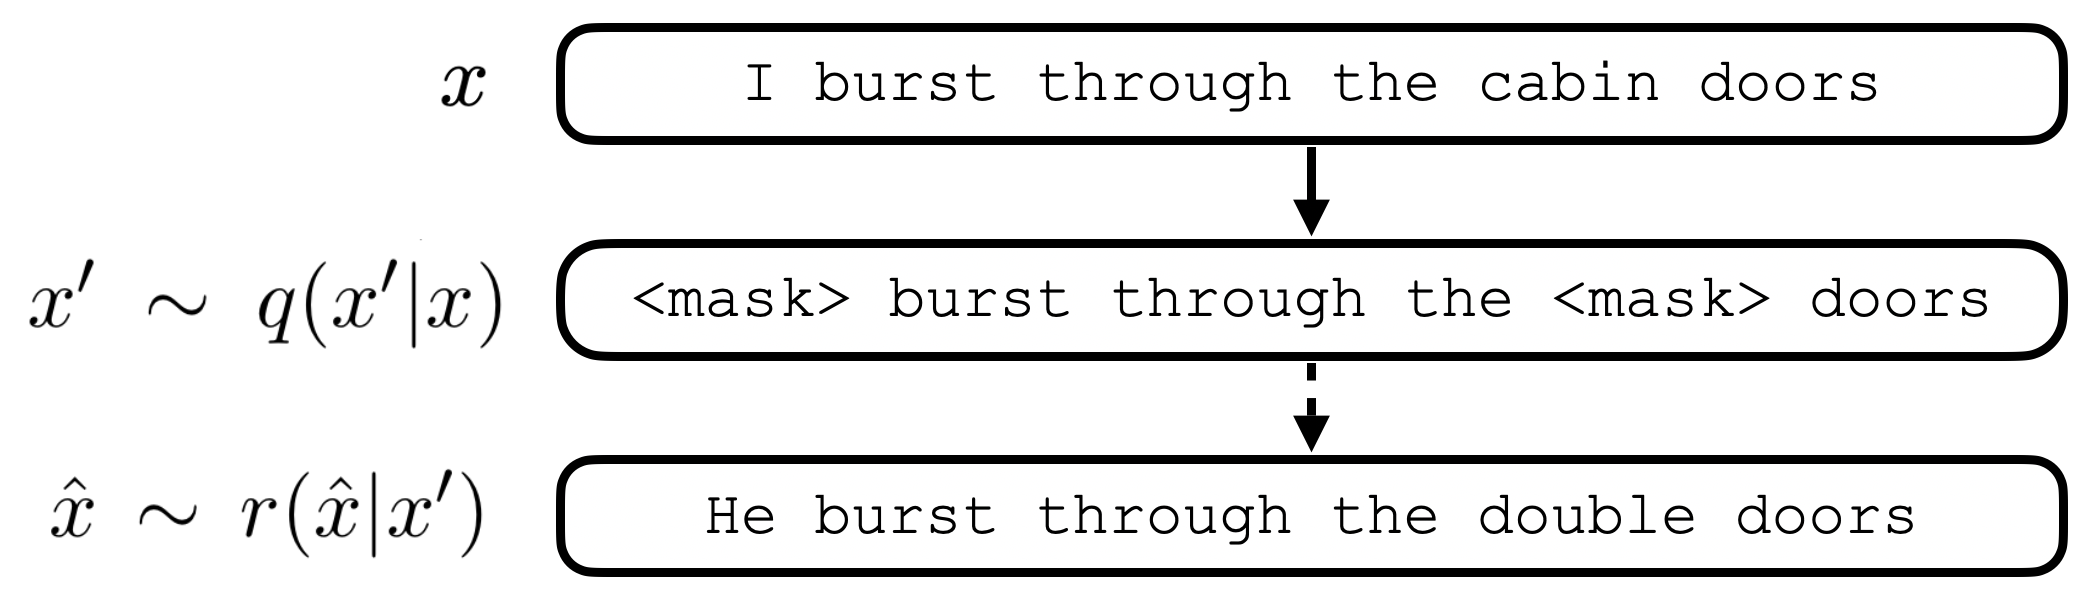
\includegraphics[scale=0.21]{img/bert_dae.png}
\caption{To sample from an MLM DAE, we apply the MLM corruption $q$ to the original sentence then reconstruct the corrupted sentence using our DAE $r$.}
\label{fig:dae_sampling}
\end{figure}

\subsection{Sampling from Denoising Autoencoders}
A denoising autoencoder (DAE) is an autoencoder trained to reconstruct a clean input $x$ from a stochastically corrupted one $x'\sim q(x'|x)$ by learning a conditional distribution $P_\theta (x| x')$ \citep{vincent2008extracting}.
We can sample from a DAE by successively corrupting and reconstructing an input using the following pseudo-Gibbs Markov chain: $x_t' \sim q(x'|x_{t-1})$, $x_t \sim P_\theta(x|x'_t).$
\comment{
\begin{align*}
    x_t' &\sim q(x'|x_{t-1})\\
    x_t &\sim P_\theta(x|x'_t) 
\end{align*}
}
As the number of training examples increases, the asymptotic distribution $\pi_n(x)$ of the generated samples approximate the true data-generating distribution $P(x)$ \citep{bengio2013generalized}.
This corruption-reconstruction process allows for sampling directly along the manifold that $P(x)$ concentrates on.

\subsection{Masked Language Models}
Recent advances in unsupervised representation learning for natural language have relied on pre-training models on a \textit{masked language modeling} (MLM) objective \citep{devlin2018, liu2019roberta}.
In the MLM objective, a percentage of the input tokens are randomly corrupted and the model is asked to reconstruct the original token given its left and right context in the corrupted sentence.
We use MLMs as DAEs \citep{lewis2019bart} to sample from the underlying natural language distribution by corrupting and reconstructing inputs (Figure \ref{fig:dae_sampling}).

\section{State Space Models are Structured Matrices}
\label{sec:ssm}


This section explores different perspectives of the state space model as a sequence transformation, and outlines properties and algorithms of such maps.
The main results of this section are about the equivalence between state space models and a family of structured matrices called semiseparable matrices,
which imply new efficiency results (\cref{thm:ssm-sss,thm:ssm-efficiency}).

\subsection{The Matrix Transformation Form of State Space Models}

Recall that our definition of an SSM is defined as a parameterized map
defined through \eqref{eq:s6}.
Our theoretical framework starts by simply writing this transformation as a matrix multiplication mapping the vectors $x \in \R^\mathtt{T} \mapsto y \in \R^\mathtt{T}$.

By definition, $h_0 = B_0 x_0$.
By induction,
\begin{align*}
  h_t &= A_t \dots A_1 B_0 x_0 + A_t \dots A_2 B_1 x_1 + \dots + A_t A_{t-1} B_{t-2} x_{t-2} + A_t B_{t-1} x_{t-1} + B_t x_t
    \\&= \sum_{s=0}^t A_{t:s}^\times B_s x_s
    .
\end{align*}

Multiplying by $C_t$ to produce $y_t$ and vectorizing the equation over $t \in [\mathtt{T}]$,
we derive the matrix transformation form of SSMs.
\begin{equation}
  \label{eq:ssm-matrix}
  \begin{aligned}
    y_t &= \sum_{s=0}^t C_t^{\top} A_{t:s}^\times B_s x_s
    \\
    y &= \mathsf{SSM}(A, B, C)(x) = Mx
    \\
    M_{ji} &\coloneqq C_j^{\top} A_{j} \cdots A_{i+1} B_{i}
  \end{aligned}
\end{equation}

\subsection{Semiseparable Matrices}

$M$ in equation \eqref{eq:ssm-matrix} is a particular representation of a class of matrices known as semiseparable matrices.
Semiseparable matrices are a fundamental matrix structure.
We first define these matrices and their properties.

\begin{definition}
  \label{def:semiseparable-rank}
  A (lower triangular) matrix $M$ is $\mathtt{N}$-semiseparable if every submatrix contained in the lower triangular portion (i.e.\ on or below the diagonal) has rank at most $\mathtt{N}$.
  We call $\mathtt{N}$ the \emph{order} or \emph{rank} of the semiseparable matrix.
\end{definition}

\cref{def:semiseparable-rank}, and other forms of related ``separable'' structure (e.g.\ quasiseparable matrices and other definitions of semiseparable matrices) are sometimes called \textbf{structured rank matrices} (or rank-structured matrices) because they are characterized by rank conditions on their submatrices.
Semiseparable matrices have many structured representations including the hierarchical semiseparable (HSS),
sequential semiseparable (SSS), and Bruhat forms~\citep{pernet2018time}.
We will primarily use the SSS form.

\subsubsection{The Sequentially Semiseparable (SSS) Representation}

\begin{definition}
  \label{def:sss}
  A lower triangular matrix $M \in \R^{\mathtt{(T,T)}}$ has a $\mathtt{N}$-\textbf{sequentially semiseparable (SSS)} representation if it can be written in the form
  \begin{equation}%
    \label{eq:sss}
    M_{ji} = C_j^{\top} A_{j} \cdots A_{i+1} B_{i}
  \end{equation}
  for vectors $B_{0}, \dots, B_{\mathtt{T}-1}, C_{0}, \dots, C_{\mathtt{T}-1} \in \R^{\mathtt{N}}$
  and matrices $A_{0}, \dots, A_{\mathtt{T}-1} \in \R^{\mathtt{(N,N)}}$.

  We define the operator $\mathsf{SSS}$ so that $M = \mathsf{SSS}(A_{0:\mathtt{T}}, B_{0:\mathtt{T}}, C_{0:\mathtt{T}})$.
\end{definition}

A fundamental result of semiseparable matrices is that they are exactly equivalent to matrices with SSS representations.
One direction can be deduced with a simple constructive proof.

\begin{lemma}
  \label{lmm:sss-rank-factor}
  An $\mathtt{N}$-SSS matrix $M$ with representation \eqref{eq:sss} is $\mathtt{N}$-semiseparable.
\end{lemma}
\begin{proof}
  Consider any off-diagonal block $M_{j:j', i':i}$ where $j' > j \ge i > i'$.
  This has an explicit rank-$\mathtt{N}$ factorization as
  \begin{equation}
    \label{eq:sss-rank-factor}
    \begin{bmatrix}
      C_j^{\top} A_{j:i'}^\times B_{i'}         & \dots & C_j^{\top} A_{j:i-1}^\times B_{i-1}   \\
      \vdots                                    &       &       \vdots      \\
      C_{j'-1}^{\top} A_{j'-1:i'}^\times B_{i'} & \dots & C_{j'-1}^{\top} A_{j'-1:i-1}^\times B_{i-1} \\
    \end{bmatrix}
    =
    \begin{bmatrix} C_j^{\top} A_{j:j}^\times \\ \vdots \\ C_{j'-1}^{\top} A_{j'-1:j}^\times \end{bmatrix}
    A_{j:i-1}^\times
    \begin{bmatrix} A_{i-1:i'}^\times B_{i'} & \cdots & A_{i-1:i-1}^\times B_{i-1} \end{bmatrix}
    .
  \end{equation}
\end{proof}
Equation \eqref{eq:sss-rank-factor} will be used extensively in deriving our fast algorithms for sequence models.
The other direction is well-established in the literature on semiseparable matrices.

\begin{proposition}
  \label{prop:sss}
  Every $\mathtt{N}$-semiseparable matrix has a $\mathtt{N}$-SSS representation.
\end{proposition}
Furthermore, note that although \cref{def:sss} involves $O(\mathtt{N}^2\mathtt{T})$ parameters for the representation (in particular to store the $A$ matrices),
it can actually be compressed down to $O(\mathtt{NT})$ parameters, which is asymptotically tight~\citep{pernet2023exact}.
Therefore in the rest of this paper we will conflate the structured matrix class (\cref{def:semiseparable-rank}) and a particular representation of it (\cref{def:sss}); we will always use this representation instead of other candidates.
In turn we will use $\mathtt{N}$-SS to refer to an $\mathtt{N}$-semiseparable matrix in SSS form.

Semiseparable matrices are a fundamental matrix structure and have many important properties.
They are deeply related to recurrences at large, and can be defined by multiple characterizations (e.g.\ \cref{def:semiseparable-rank,def:sss}) which reveal different connections and efficient algorithms for them.
We mention some of their other properties in \cref{sec:ssm:properties}.

\begin{remark}
  The notion of semiseparability is very broad and many similar but subtlely different definitions appear in the literature;
  our definitions may differ slightly from other conventions.
  First, because we are primarily concerned with causal or autoregressive settings in this paper,
  we have restricted the definition of semiseparability to the triangular case;
  \cref{def:semiseparable-rank} more formally might be called $(\mathtt{N},0)$-semiseparability by some authors.
  Some authors may also instead refer to it as a form of quasiseparability~\citep{eidelman1999new,pernet2016computing}.
  See \citet{vandebril2005bibliography} for a brief survey.
\end{remark}

\subsubsection{1-Semiseparable Matrices: the Scalar SSM Recurrence}
\label{sec:ssm:1-ss}

We will single out the special case of $1$-SS matrices.
Note that in this case, the $C_j$ and $B_i$ are scalars, and can be factored out of the SSS representation \eqref{eq:sss}
(we also use lower-case to emphasize that the parameters are scalars in this case)
\begin{align*}%
  \mathsf{SSS}(a, b, c) = \mathsf{diag}(c) \cdot M \cdot \mathsf{diag}(b) \qquad \text{where} \qquad M_{ji} = a_{j:i}^\times
  .
\end{align*}

Since diagonal matrices are easy to handle (e.g.\ multiplication by a diagonal matrix is the same as elementwise scalar multiplication),
we can ignore these terms.
Thus our basic representation of a 1-SS matrix is $M_{ji} = a_{j:i}$ or
\begin{equation}%
  \label{eq:1ss}
  M =
  \mathsf{1SS}(a_{0:T}) \coloneqq
  \begin{bmatrix}
    1 & \\
    a_1 & 1 & \\
    a_2a_1 & a_2 & 1 \\
    \vdots & \vdots & \ddots & \ddots \\
    a_{T-1}\dots a_1 & a_{T-1}\dots a_2 & \dots & a_{T-1} & 1 \\
  \end{bmatrix}
  .
\end{equation}

The importance of 1-SS matrices lies in their equivalence to the minimal form of a scalar recurrence -- the case of a degenerate SSM with state dimension $\mathtt{N}=1$ and no $(B, C)$ projections.
Note that multiplication $y = Mx$ can be computed by the recurrence
\begin{equation}
  \label{eq:1ss-recurrence}
  \begin{aligned}
    y_t &= a_{t:0}x_0 + \dots + a_{t:t}x_t \\
        &= a_t \left(a_{t-1:0}x_0 + \dots + a_{t-1:t-1}x_{t-1}\right) + a_{t:t}x_t \\
        &= a_t y_{t-1} + x_t
        .
  \end{aligned}
\end{equation}
We thus also refer to matrix multiplication by $1$-SS matrices as the \textbf{scalar SSM recurrence} or the \texttt{cumprodsum} (cumulative product sum; a generalization of cumulative product and cumulative sum) operator.
As the fundamental form of recurrence, multiplication by 1-SS matrices is important
as a building block for our main algorithms.

We emphasize that one of the central themes of this paper is that \emph{many algorithms on sequence models can be reduced to structured matrix multiplication algorithms}.
1-SS matrices exemplify this connection: there are many fast algorithms for computing the primitive scalar recurrence or \texttt{cumprodsum} operator,
and all of them turn out to be equivalent to different structured factorization of 1-SS matrices.
We dedicate \cref{sec:scan} to these algorithms for 1-SS matrix multiplication.

\subsection{State Space Models are Semiseparable Matrices}
Recall that our definition of an SSM is defined as a parameterized map
defined through \cref{def:sequence-transformation}.
The connection between SSMs and semiseparable matrices follows from simply writing this transformation as a matrix multiplication mapping the vectors $x \mapsto y \in \R^\mathtt{T}$.

Equation \eqref{eq:ssm-matrix} directly establishes the link between state space models and the sequentially semiseparable representation, which in turn are equivalent to semiseparable matrices in general (\cref{lmm:sss-rank-factor,prop:sss}).
\begin{theorem}
  \label{thm:ssm-sss}
  The state space model transformation $y = \mathsf{SSM}(A, B, C)(x)$ with state size $\mathtt{N}$ is identical to matrix multiplication by an $\mathtt{N}$-SS matrix in sequentially semiseparable representation $y = \mathsf{SSS}(A, B, C) \cdot x$.
\end{theorem}

In other words the sequence transformation operator $\mathsf{SSM}$ (\cref{def:ssm}) coincides with the matrix construction operator $\mathsf{SSS}$ (\cref{def:sss}),
and we use them interchangeably (or sometimes $\mathsf{SS}$ as shorthand).
Furthermore---by a twist of fate---structured state space models and sequentially semiseparable matrices have the same acronyms, underscoring their equivalence!
Conveniently we can use any of these acronyms SSM (state space model or semiseparable matrix), SSS (structured state space or sequentially semiseparable), or SS (state space or semiseparable) interchangeably to unambiguously refer to either concept.
However, we will generally use the convention that SSM refers to state space model, SS refers to semiseparable, and SSS refers to sequentially semiseparable.


\cref{fig:ssm-semiseparable} illustrates the sequence transformation perspective of state space models as semiseparable matrices.
\begin{figure}[!t]
  \centering
  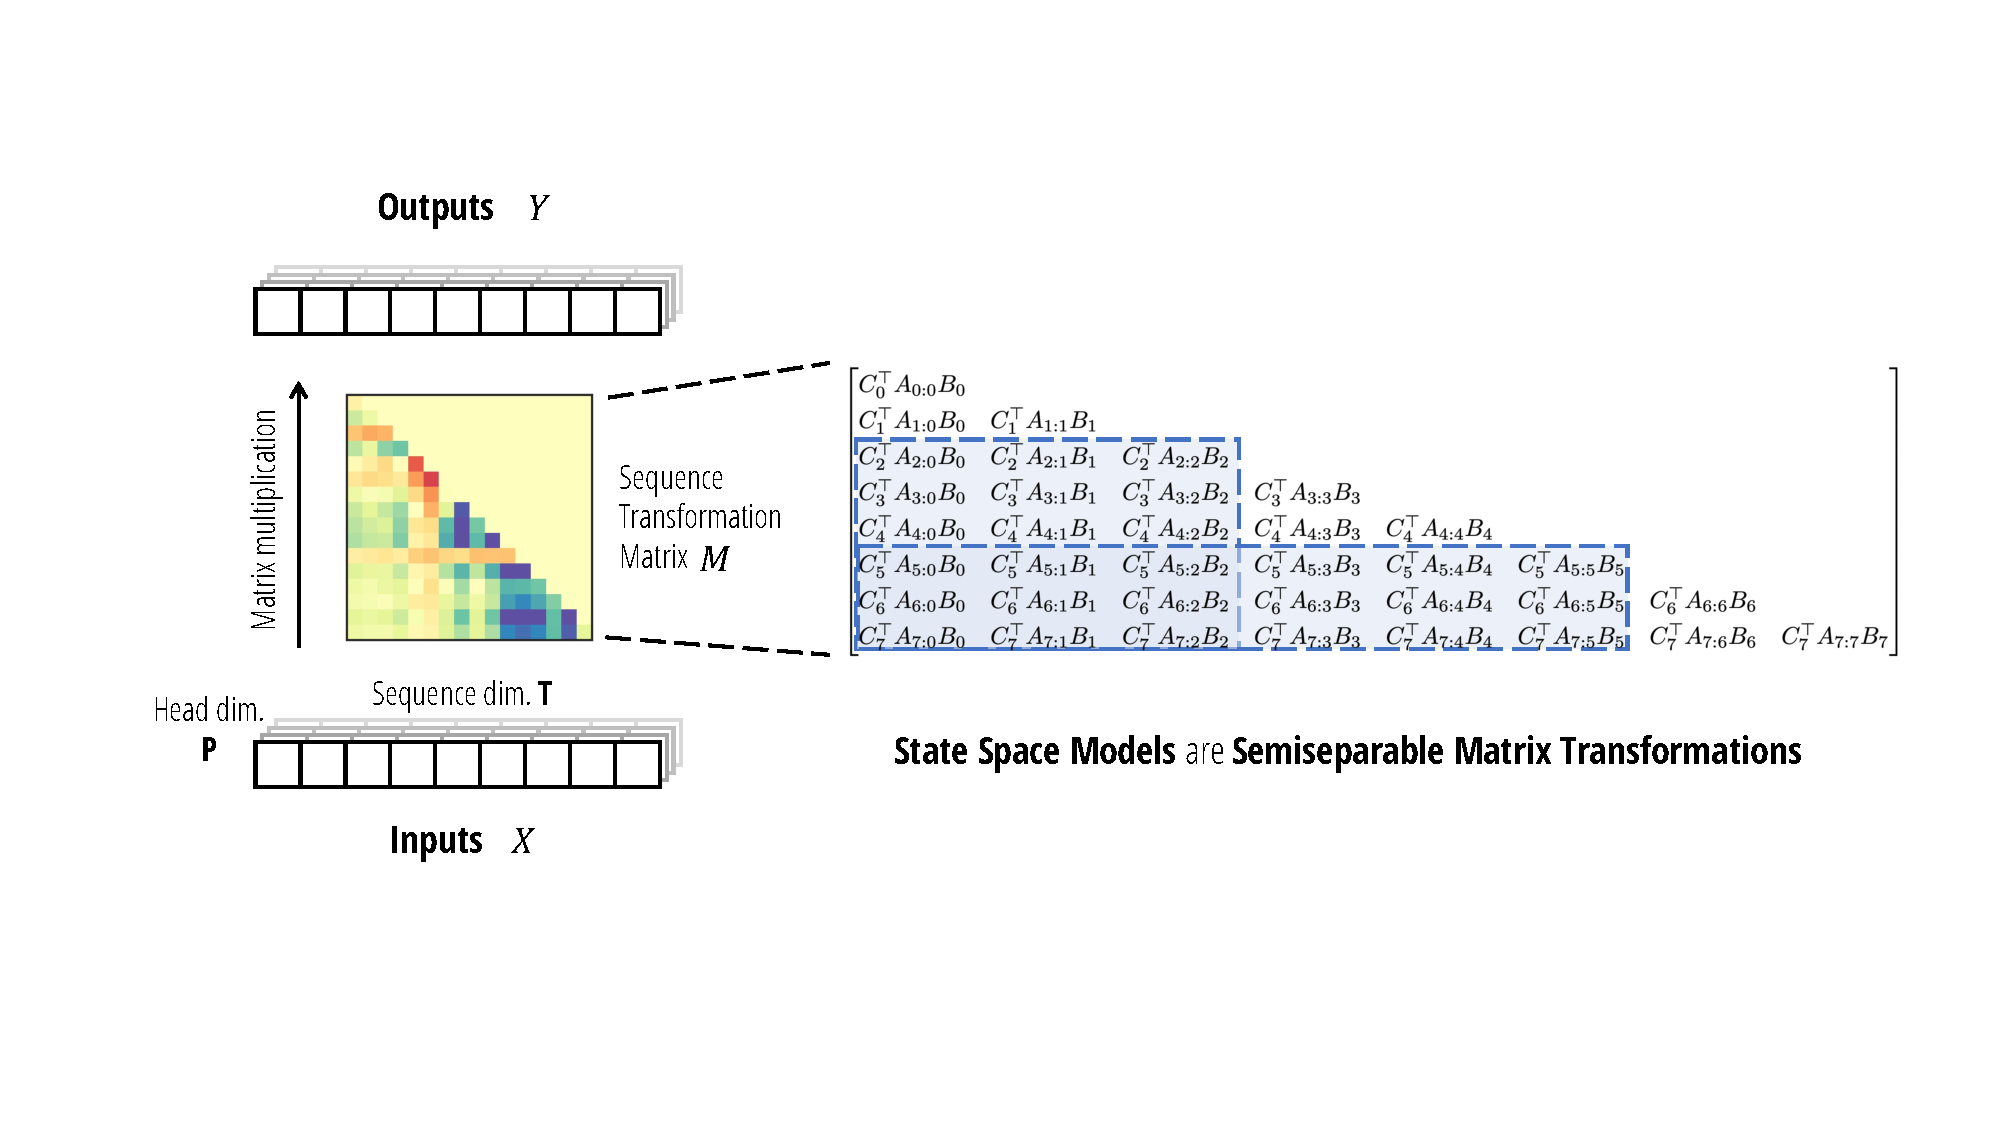
\includegraphics[width=\linewidth]{fig/semiseparable.pdf}
  \caption{
    (\textbf{State Space Models are Semiseparable Matrices}.)
    As sequence transformations, state space models can be represented as a matrix transformation $M \in \mathbb{R}^{\mathtt{(T,T)}}$ acting on the sequence dimension $\mathtt{T}$,
    sharing the same matrix for each channel in a head (\emph{Left}).
    This matrix is a semiseparable matrix (\emph{Right}), which is a rank-structured matrix where every submatrix contained on-and-below the diagonal (\emph{Blue}) has rank at most $\mathtt{N}$,
    equal to the SSM's state dimension.
  }
  \label{fig:ssm-semiseparable}
\end{figure}


\subsection{Computing State Space Models through Structured Matrix Algorithms}
\label{sec:ssm:algorithms}

The reason \cref{thm:ssm-sss} is important is that it will allow us to \emph{reduce the problem of efficient computation of SSMs (and other sequence models) into efficient algorithms for structured matrix multiplication}.
We briefly provide an overview and defer our main new algorithm to \cref{sec:efficient}, after showing the equivalence of SSMs to other sequence models in
\cref{sec:attention,sec:ssd}.

As previously defined, semiseparable matrices (i.e.\ rank-structured matrices) are a classical type of structured matrix:
\begin{enumerate}[label=(\roman*)]
  \item They have compressed representations such as the SSS form which has only $O(\mathtt{T})$ instead of $O(\mathtt{T}^2)$ parameters.
  \item They have fast algorithms operating directly on the compressed representation.
\end{enumerate}
Furthermore, the parameterization and matrix multiplication cost can be tight in the semiseparable order.
\begin{proposition}[\citet{pernet2023exact}]
  \label{prop:ss-mvm}
  An $\mathtt{N}$-SS matrix of size $\mathtt{T}$ can be represented in $O(\mathtt{NT})$ parameters and has matrix-vector multiplication in time and space $O(\mathtt{NT})$.
\end{proposition}

For example, 1-SS matrices illustrate the essence of this connection.
The matrix $M = \mathsf{1SS}(a)$ is defined by exactly $\mathtt{T}-1$ parameters $a_{0:\mathtt{T}-1} = a_1, \dots, a_{\mathtt{T}-1}$,
and can be computed in $O(\mathtt{T})$ time by following the scalar recurrence \eqref{eq:1ss-recurrence}.




\subsubsection{The Linear (Recurrent) Mode}
\label{sec:ssm:algorithms:linear}

\cref{prop:ss-mvm} can be easily seen in the case of diagonal structured SSMs (S4D~\citep{gu2022parameterization}),
simply by leveraging the state space model formulation \eqref{eq:s6} and unrolling the recurrence.
We provide the formal tensor-contraction algorithm in \eqref{eq:ssm-diagonal}, where the dimension $\mathtt{S}$ is equal to $\mathtt{T}$%
\footnote{A different symbol is required for the contraction notation.}.
\begin{subequations}
  \label{eq:ssm-diagonal}
  \begin{align}
    \label{eq:ssm-diagonal:1}
    Z &= \mathsf{contract}(\mathtt{SP},\mathtt{SN} \to \mathtt{SPN})(X, B) & \mathtt{(S,P,N)} \\
    \label{eq:ssm-diagonal:2}
    H &= \mathsf{contract}(\mathtt{TSN},\mathtt{SPN} \to \mathtt{TPN})(L, Z) & \mathtt{(T,P,N)} \\
    \label{eq:ssm-diagonal:3}
    Y &= \mathsf{contract}(\mathtt{TN},\mathtt{TPN} \to \mathtt{TP})(C, H) & \mathtt{(T,P)}
  \end{align}
\end{subequations}
Here, $L \in \R^{(\mathtt{T},\mathtt{T})}$ is defined as $\mathsf{1SS}(A)$, or in other words $L_{0:\mathtt{T},0:\mathtt{T}} = \mathsf{1SS}(A_{0:\mathtt{T}})$ for $i \in [\mathtt{N}]$.
This algorithm involves three steps corresponding to \eqref{eq:s6}:
\begin{enumerate}[label=(\roman*)]
  \item \emph{expanding} the input $X$ by the input matrix $B$ \eqref{eq:ssm-diagonal:1},
  \item unrolling independent scalar SSM recurrences \eqref{eq:ssm-diagonal:2}, and
  \item \emph{contracting} the hidden state $H$ by the output matrix $C$ \eqref{eq:ssm-diagonal:3}.
\end{enumerate}
Note that we have used the equivalence between scalar SSMs and 1-SS matrices in step \eqref{eq:ssm-diagonal:2}.

\begin{remark}
  We note that \eqref{eq:ssm-diagonal} is a special case of the Mamba (S6) model.
  however, a naive implementation is slow because of the expanded tensors $Z$ and $H$ of size $\mathtt{(T,P,N)}$;
  \citet{gu2023mamba} introduced a hardware-aware implementation to avoid materializing these tensors.
\end{remark}



Surprisingly, \cref{thm:ssm-sss} and \cref{prop:ss-mvm} immediately imply that all SSMs have the same asymptotic efficiency as algorithm \eqref{eq:ssm-diagonal}.
\begin{theorem}
  \label{thm:ssm-efficiency}
  Any state space model (\cref{def:ssm}) of state size $\mathtt{N}$ on sequence length $\mathtt{T}$ can be computed in time $O(\mathtt{TN})$ (not accounting for potential preprocessing).
\end{theorem}
We note that this result is new to the structured SSM literature.
In particular, given dense unstructured $A_t$ matrices, the total representation alone seems to be of size $O(\mathtt{TN}^2)$.
Thus \cref{thm:ssm-efficiency} states the non-trivial result that with a pre-processing step, even an unstructured SSM can be computed optimally efficiently,
with upper bound matching the lower bound $O(\mathtt{TN})$ given by the size of $B$ and $C$.

\begin{remark}
  \cref{thm:ssm-efficiency} is perhaps not too surprising in light of the fact that almost all dense matrices over $\R^{\mathtt{(N,N)}}$ are diagonalizable over $\mathbb{C}$,
  leading to the result that \emph{almost all} dense real SSMs are equivalent to a diagonal complex SSM.
  This fact underlies the reason why diagonal SSMs are the most popular form of structured SSM~\citep{gupta2022diagonal,gu2022parameterization,smith2023s5}.
  However, \cref{thm:ssm-efficiency} implies the much stronger result for \emph{all} real SSMs (not just the diagonalizable ones), as well as dense SSMs over other fields (including $\mathbb{C}$ itself).
\end{remark}

In practice, efficiently computable SSMs still require additional structure on $A$,
particularly to avoid the expensive preprocessing step (which both has order $\mathtt{N}$ extra FLOPs and involves hardware-inefficient operations such as singular value decompositions).
These structures are the focus of past work on structured SSMs (e.g.\ S4(D) and Mamba) as well as our new algorithms.
In particular, when slightly stronger structure is imposed on $A$, we will design very hardware-efficient algorithms through block decompositions of the SSM matrix $M = \mathsf{SSS}(A, B, C)$ in \cref{sec:efficient}.

\subsubsection{The Quadratic (Naive) Mode}

We note that there is another way to compute an SSM exposed by our new matrix point of view.
A naive computation of the matrix SSM representation \eqref{eq:ssm-matrix} involves simply materializing the sequence transformation matrix $M=\mathsf{SSS}(A, B, C)$.
This is a $\mathtt{(T,T)}$ matrix, and therefore this naive algorithm will scale quadratically in sequence length.
However, when the sequence length $\mathtt{T}$ is short, this can actually be more efficient than the linear algorithm due to constant factors and the hardware-friendliness of the computation pattern (e.g. leveraging matrix-matrix multiplications).
In fact, for a particular case of structured SSMs, this looks very similar to a quadratic attention computation (\cref{sec:ssd}).




\subsubsection{Summary}

Many sequence models are explicitly motivated or defined as matrix sequence transformations --
most notably Transformers, where the matrix mixer is the attention matrix.
On the other hand, RNNs and SSMs have not previously been described in this way.
By providing an explicit \emph{matrix transformation} form of state space models,
we reveal new ways of understanding and using them.
From a computational perspective, any method of computing the forward pass of a state space model can be
viewed as a matrix multiplication algorithm on semiseparable matrices.
The semiseparable matrix perspective provides one lens into state space duality (SSD),
where the dual modes respectively refer to a linear-time semiseparable matrix multiplication algorithm and quadratic-time naive matrix multiplication.

Moreover, leveraging the rich structure of semiseparable matrices can lead to even better algorithms and more insights (e.g. \cref{sec:efficient,sec:scan}).
In \cref{sec:ssm:properties}, we describe some additional properties of semiseparable matrices.



\section{Structured Masked Attention: Generalizing Linear Attention \texorpdfstring{\\}{} with Structured Matrices}
\label{sec:attention}

%



In this section we revisit the linear attention framework from first principles.
The main results in this section are a simple tensor-contraction-based proof of linear attention (\cref{prop:linear-attention}),
and our generalized abstraction of structured masked attention in \cref{def:sma}.
\iftoggle{arxiv}{
We note that this section derives the main duality results from a different direction than state space models and can be read completely independently of \cref{sec:ssm}.
}{}

\begin{itemize}
  \item \cref{sec:masked-attention} sets up our framework for variants of attention, with a particular focus on kernel attention and masked kernel attention.
  \item \cref{sec:linear-attention} provides our first main attention result, a simple proof of linear attention through the lens of tensor contractions.
  \item \cref{sec:structured-attention} defines structured masked attention, our generalization of prior attention variants through structured matrices.
\end{itemize}

\subsection{The Attention Framework}
\label{sec:masked-attention}

\subsubsection{Attention}
The basic form of (single-head) attention is a map on three sequences of vectors $(Q, K, V) \mapsto Y$.
\begin{equation}
  \label{eq:kernel-attention}
  \begin{aligned}%
    Q &= \mathsf{input} & \mathtt{(T,N)} \\
    K &= \mathsf{input} & \mathtt{(S,N)} \\
    V &= \mathsf{input} & \mathtt{(S,P)} \\
    G &= QK^\top        & \mathtt{(T,S)} \\
    M &= f(G)           & \mathtt{(T,S)} \\
    Y &= GV             & \mathtt{(T,P)} \\
  \end{aligned}
\end{equation}
We use ``shape annotations'' to indicate the dimensions of tensors, e.g.\ $Q \in \R^{\mathtt{(T,N)}}$.
In this general form, $\mathtt{S}$ and $\mathtt{T}$ represent \emph{source} and \emph{target} sequence lengths,
$\mathtt{N}$ represents the \emph{feature dimension}, and $\mathtt{P}$ represents the \emph{head dimension}.

The most common variant of \textbf{softmax attention} uses a softmax activation $f=\mathsf{softmax}$ to normalize the rows of the $G$ matrix.

\subsubsection{Self-Attention}
Our treatment is motivated by the most important case of self-attention, where
\begin{enumerate}[label=(\roman*)]
  \item the source and target sequences are the same (i.e.\ $\mathtt{S}=\mathtt{T}$),
  \item usually the feature and head dimensions are the same (i.e.\ $\mathtt{N}=\mathtt{P}$),
  \item and $Q, K, V$ are generated by linear projections on the same input vector ($Q = W_Q \cdot X, K = W_K \cdot X, V = W_V \cdot X$).
\end{enumerate}
However, our presentation abstracts away these choices and begins from the $Q, K, V$ matrices.

\begin{remark}
  Our focus is on the self-attention case with equal head and feature dimensions (i.e.\ $\mathtt{S}=\mathtt{T}$ and $\mathtt{N}=\mathtt{P}$),
  which should be used as the running example.
  We define the general formulation of attention not only so that our framework captures variants such as cross-attention,
  but also because separating the notation for dimensions (e.g.\ $\mathtt{S}$ and $\mathtt{T}$) makes the contraction notation proofs
  of our main results in this section more clear.
\end{remark}

\begin{remark}
  \label{rmk:attention-input}
  While attention is usually framed as an operation on these three inputs $Q, K, V$ which are viewed symmetrically,
  the input and output dimensions in \eqref{eq:kernel-attention} indicate otherwise.
  In particular, the feature dimension $\mathtt{N}$ is not present in the output;
  therefore in the case when $\mathtt{S}=\mathtt{T}$ (e.g.\ self-attention),
  we view $V$ as the main input, so that \eqref{eq:kernel-attention} defines a proper sequence transformation $V \mapsto Y$ (\cref{def:sequence-transformation}).
\end{remark}

\subsubsection{Kernel Attention}
\label{sec:attention:kernel}

The step where the softmax function is applied to the Gram matrix $G$ can be decomposed into two parts:
\begin{enumerate}
  \item Exponentiating the $G$ matrix.
  \item Normalizing the $G$ matrix on the $\mathtt{S}$ axis.
\end{enumerate}
We can ignore the normalization term for now, as it amounts to simply passing in $V=1$ and dividing\iftoggle{arxiv}{ (we revisit this in \cref{sec:architecture:kernels})}{}.
The exponentiation term can be viewed as a kernel transformation:
there is an (infinite-dimensional) feature map $\varphi$ such that $\exp(QK^{\top}) = \varphi(Q)\varphi(K)^{\top}$.
By abstracting away the feature map into the definition of $Q$ and $K$ itself (i.e.\ define $Q, K$ as the post-transformed versions),
we can ignore the softmax transformation, and assume that $Q, K$ are arbitrarily generated by kernel feature maps and potentially $\mathtt{N} \neq \mathtt{P}$.

Many instantiations of kernel attention have been proposed, including:
\begin{itemize}
  \item The original Linear Attention \citep{katharopoulos2020transformers} defines the kernel feature map as an arbitrary pointwise activation function, such as $x \mapsto 1+\mathsf{elu}(x)$.
  \item Random Feature Attention (RFA)~\citep{peng2021random} chooses the kernel feature map to approximate softmax attention (i.e. the $\exp$ feature map) using the random Fourier feature approximation of Gaussian kernels~\citep{rahimi2007random}. This involves random projections (i.e.\ multiplying $Q$ and $K$ by a random projection $W$ and applying the activation $x \mapsto (\cos(x), \sin(x))$.
%
  \item Performer~\citep{choromanski2021rethinking} proposes the fast attention via positive orthogonal random features (FAVOR+).
    The positive random features (PRF) part chooses the kernel feature map to be a random projection followed by the feature map $x \mapsto 2^{-1/2}(\exp(x), \exp(-x))$.
    This choice is motivated so that the kernel elements are positive-valued and provably approximates the softmax attention. [It also proposes choosing the random projections in orthogonal directions, which we do not consider.]
  \item cosFormer~\citep{qin2022cosformer} augment RFA with a cosine reweighting mechanism that incorporates positional information to emphasize locality.
    This effectively passes $Q_t,K_t$ through the feature map $x \mapsto (x \cos(\pi t / 2T), \sin(\pi t / 2T))$.
  \item Linear Randomized Attention~\citep{zheng2022linear} generalize RFA from the perspective of importance sampling, and generalize it to provide better estimates of the full softmax kernel (rather than just the $\exp$-transformed numerator).
\end{itemize}

Other related attention variants include Linformer~\citep{wang2020linformer} and Nystr\"{o}former~\citep{xiong2021nystromformer}, which both use low-rank approximations of the attention matrix $M$ (and are thus compatible with equation \eqref{eq:kernel-attention}), through random projections (Johnson-Lindenstrauss) and kernel approximation (the Nystr\"{o}m method) respectively.


\subsubsection{Masked (Kernel) Attention}

%

Let $L$ be a mask of shape $\mathtt{(T,S)}$.
Most commonly, in the \emph{autoregressive} self-attention case when $\mathtt{S}=\mathtt{T}$,
$L$ may be a lower-triangular matrix of $1$'s representing a \emph{causal mask}.
Besides enforcing causality, many other types of masks can be applied -- in particular various sparsity patterns such as banded, dilated, or block diagonal -- which are motivated by reducing the complexity of dense attention. %

Masked attention is usually written in matrix notation as
\begin{equation}%
  \label{eq:sha-quad-matrix}
  y = (L \circ (QK^\top)) \cdot V
  .
\end{equation}
More precisely, with shape annotations and breaking this down into the precise sequence of computations:
\begin{equation}
  \label{eq:sha-quad-0}
  \begin{aligned}%
    G &= QK^\top & \mathtt{(T,S)} \\
    M &= G \circ L & \mathtt{(T,S)} \\
    Y &= M V & \mathtt{(T,P)}
  \end{aligned}
\end{equation}

Our improved derivation of attention variants in this section starts by noticing that this formula can be written as a \emph{single contraction}:
\begin{equation}
  \label{eq:sha}
  Y = \mathsf{contract}(\mathtt{TN},\mathtt{SN},\mathtt{SP},\mathtt{TS} \to \mathtt{TP})(Q, K, V, L)
\end{equation}

and the algorithm in \eqref{eq:sha-quad-0} can be reframed as computing \eqref{eq:sha} by a particular ordering of pairwise contractions
\begin{subequations}
  \label{eq:sha-quad}
  \begin{align}%
    \label{eq:sha-quad:1}
    G &= \mathsf{contract}(\mathtt{TN, SN} \to \mathtt{TS})(Q, K) && \qquad \mathtt{(T,S)} \\
    \label{eq:sha-quad:2}
    M &= \mathsf{contract}(\mathtt{TS, TS} \to \mathtt{TS})(G, L) && \qquad \mathtt{(T,S)} \\
    \label{eq:sha-quad:3}
    Y &= \mathsf{contract}(\mathtt{TS, SP} \to \mathtt{TP})(M, V) && \qquad \mathtt{(T,P)}
  \end{align}
\end{subequations}

\subsection{Linear Attention}
\label{sec:linear-attention}

Linear attention, and many other variants of efficient attention, is often motivated by changing the order of matrix associativity in the core attention computation $(QK^\top)V = Q(K^\top V)$.
However when the mask is added, the derivation is somewhat less straightforward (for example, the original paper~\citep{katharopoulos2020transformers} and variants~\citep{sun2023retentive} state the formula without proof).

Roughly, the linear attention method claims that the following formula
is equivalent to \eqref{eq:sha-quad-matrix}, which must be verified by expanding the sum and tracking indices carefully.
\begin{equation}
  \label{eq:sha-lin-matrix}
  Y = Q \cdot \mathsf{cumsum}(K^\top V)
\end{equation}

\begin{proposition}[\citep{katharopoulos2020transformers}]
  \label{prop:linear-attention}
  Autoregressive kernel attention, i.e.\ masked kernel attention with the causal mask, can be computed in $O(T)$ time by a recurrence taking constant time per step.
\end{proposition}

\subsubsection{A Tensor Contraction Proof of Linear Attention}

We present a simple and rigorous derivation of linear attention that will also immediately reveal how to generalize it.
The main idea is to perform the contraction \eqref{eq:sha} in an alternate order.
We avoid ambiguous matrix notation and work directly with contraction notation:
\begin{subequations}
  \label{eq:sha-lin}
  \begin{align}
    \label{eq:sha-lin:1}
    Z &= \mathsf{contract}(\mathtt{SP},\mathtt{SN} \to \mathtt{SPN})(V, K) & \mathtt{(S,P,N)} \\
    \label{eq:sha-lin:2}
    H &= \mathsf{contract}(\mathtt{TS},\mathtt{SPN} \to \mathtt{TPN})(L, Z) & \mathtt{(T,P,N)} \\
    \label{eq:sha-lin:3}
    Y &= \mathsf{contract}(\mathtt{TN},\mathtt{TPN} \to \mathtt{TP})(Q, H) & \mathtt{(T,P)}
  \end{align}
\end{subequations}

Intuitively, we interpret this contraction order as follows.

The first step \eqref{eq:sha-lin:1} performs an ``expansion'' into more features, by a factor of the feature dimension $\mathtt{N}$.
The third step \eqref{eq:sha-lin:3} contracts the expanded feature dimension away.
If $K$ is viewed as the input (\cref{rmk:attention-input}),
then $V$ and $Q$ perform the expansion and contraction, respectively.

The second step is the most critical, and explains the \emph{linear} part of linear attention.
First notice that \eqref{eq:sha-lin:2} is just a direct matrix multiplication by $L$ (since the $\mathtt{(P,N)}$ axes can be flattened).
Also note that this is the only term that involves both $\mathtt{T}$ and $\mathtt{S}$ axes,
hence should have $\Omega(\mathtt{TS})$ complexity (i.e.\ quadratic in sequence length).
However, when the mask $L$ is the standard causal attention mask (lower triangular $1$'s),
matrix-vector multiplication by $L$ is identical to a feature-wise cumulative sum
\begin{align*}%
  y = \begin{bmatrix} 1 \\ \vdots & \ddots \\ 1 & \dots & 1 \end{bmatrix} x
  \quad\iff\quad
  \begin{aligned}
    y_0 &= x_0 \\
    y_t &= y_{t-1} + x_t
  \end{aligned}
  .
\end{align*}


%

\subsection{Structured Masked Attention}
\label{sec:structured-attention}

With the tensor contraction perspective of masked attention \eqref{eq:sha-lin},
we can immediately see that the crux of the original linear attention is the fact that \emph{matrix-vector multiplication by the causal mask is equivalent to the cumulative sum operator}.

However, we observe that there is no reason the attention mask has to be all $1$'s.
All that is necessary for linear attention to be fast is for $L$ to be a \emph{structured matrix},
which by definition are those that have fast matrix multiplication\iftoggle{arxiv}{ (\cref{sec:overview:structured-matrix})}{}.
In particular, we can use \emph{any mask matrix} $L$ that has sub-quadratic (ideally linear) matrix-vector multiplication,
which would have the same complexity as standard linear attention by speeding up the bottleneck equation \eqref{eq:sha-lin:2}.

\begin{definition}%
  \label{def:sma}
  \textbf{Structured masked attention (SMA)} (or \textbf{structured attention} for short) is defined as a \emph{function} on queries/keys/values $Q, K, V$ as well as any \emph{structured matrix} $L$ (i.e.\ has sub-quadratic matrix multiplication), through the 4-way tensor contraction
  \begin{align*}
    Y = \mathsf{contract}(\mathtt{TN},\mathtt{SN},\mathtt{SP},\mathtt{TS} \to \mathtt{TP})(Q, K, V, L)
    .
  \end{align*}
  The SMA \textbf{quadratic mode algorithm} is the sequence of pairwise contractions defined by \eqref{eq:sha-quad},
  which corresponds to the standard (masked) attention computation.

  The SMA \textbf{linear mode algorithm} is the sequence of pairwise contractions defined by \eqref{eq:sha-lin},
  where step \eqref{eq:sha-lin:2} is optimized through the subquadratic structured matrix multiplication.
\end{definition}
We can instantiate structured masked attention to any given class of matrix structure.
Some examples include (\cref{fig:sma}):
\begin{itemize}
  \item Linear attention uses a causal mask.
  \item RetNet~\citep{sun2023retentive} uses a decay mask $L_{ij} = \gamma^{i-j} \cdot \mathbb{I}[j \ge i]$ for some decay factor $\gamma \in [0, 1]$.
  \item The decay mask could be generalized to a Toeplitz matrix $L_{ij} = \alpha_{i-j}$ for some learnable (or input-dependent) set of parameters $\alpha \in \mathbb{R}^\mathtt{T}$. This can be interpreted as a form of relative positional encoding, reminiscent of other methods such as AliBi~\citep{press2022train} but multiplicative instead of additive.
  \item Another variant could use a Fourier matrix $L_{ij} = \omega^{ij / \mathtt{T}}$ to encode positional structure a different way.
\end{itemize}
In \cref{sec:ssd}, we consider semiseparable SMA, which defines our main SSD model.

\iftoggle{arxiv}{
\begin{figure}[!t]
  \centering
  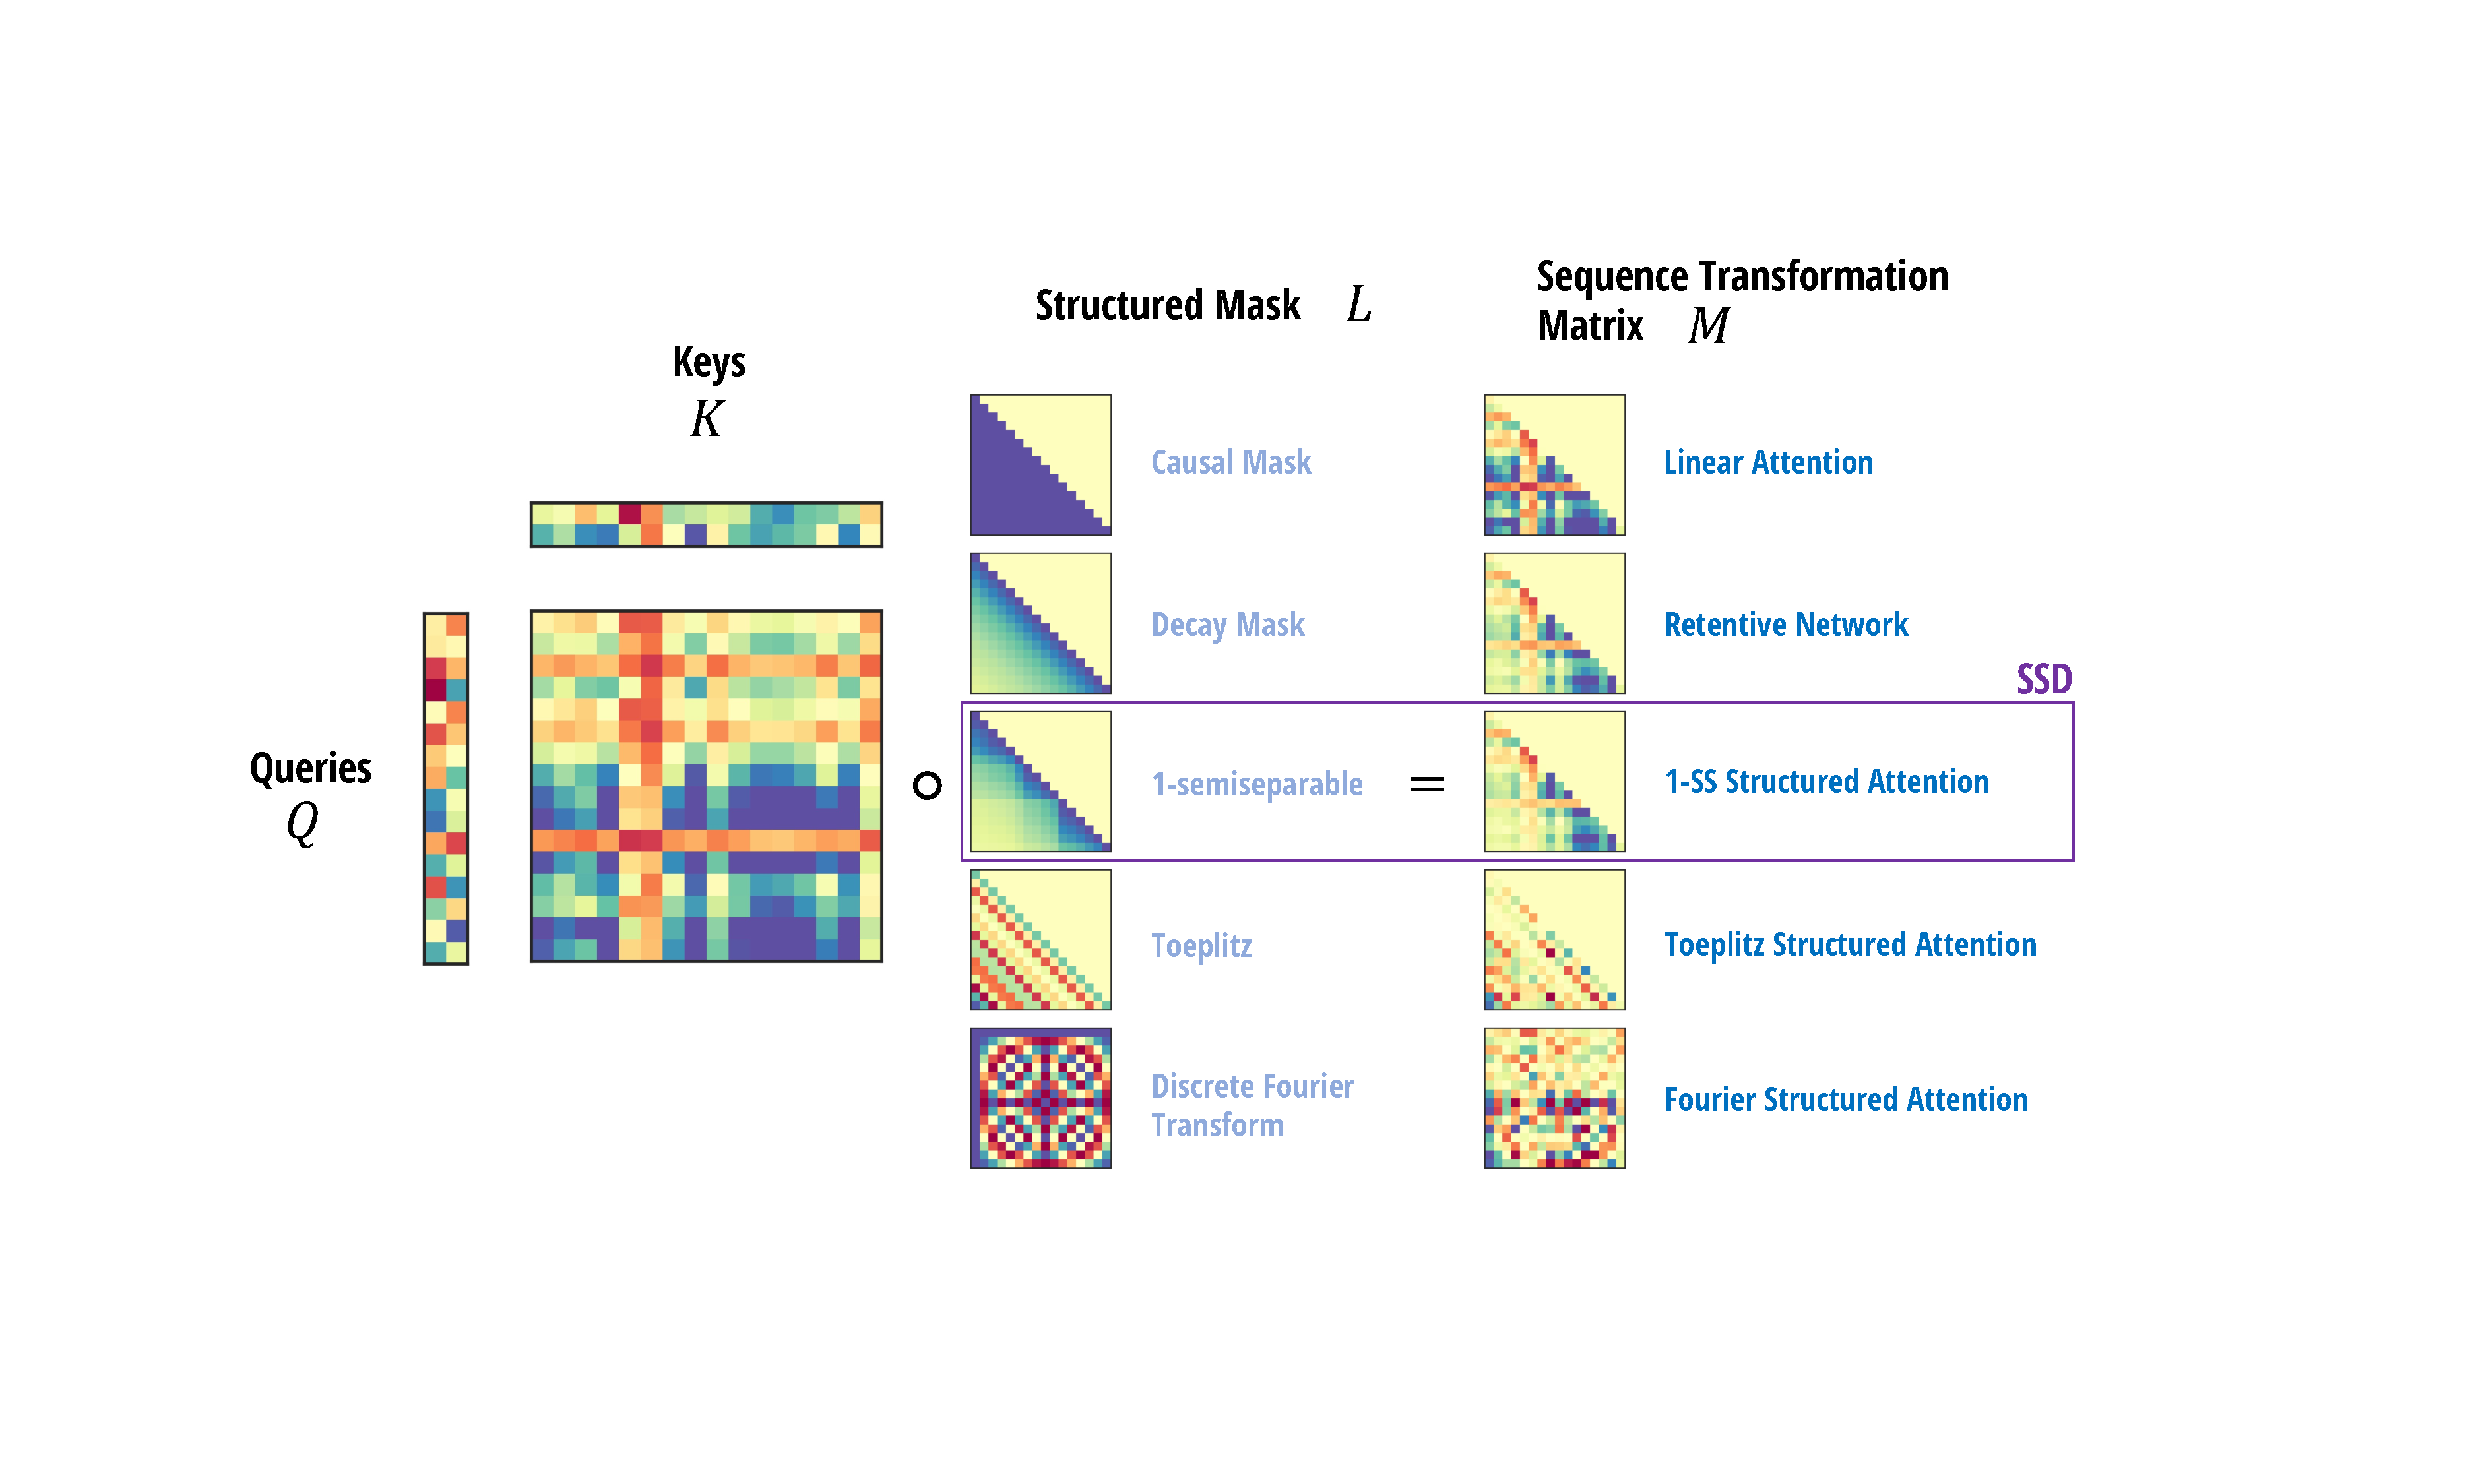
\includegraphics[width=0.9\linewidth]{fig/sma.pdf}
  \caption{
    (\textbf{Structured Masked Attention}.)
    SMA constructs a masked attention matrix $M = QK^\top \circ L$ for any structured matrix $L$, which defines a matrix sequence transformation $Y = MV$.
    All instances of SMA have a dual subquadratic form induced by a different contraction ordering, combined with the efficient structured matrix multiplication by $L$.
    Previous examples include Linear Attention~\citep{katharopoulos2020transformers} and RetNet~\citep{sun2023retentive}.
    Beyond SSD (1-semiseparable SMA), the focus of this paper, many other potential instantiations of structured attention are possible.
  }
  \label{fig:sma}
\end{figure}
}{}


\subsubsection{Summary: The Dual Forms of Masked Attention}

Standard (masked kernel) attention is often conflated between a function and an algorithm.
Separating this distinction presents a clear way to understand different variants of attention.
\begin{itemize}
  \item We view \textbf{masked attention} as a particular \emph{function}~\eqref{eq:sha}.
  \item The standard \textbf{quadratic attention} computation \eqref{eq:sha-quad} can be viewed as an \emph{algorithm} to compute the function.
  \item \textbf{Linear attention} \eqref{eq:sha-lin} is an alternate algorithm to compute the same function.
\end{itemize}

Moreover, in this case
\begin{itemize}
  \item The masked attention function is simply a particular \emph{contraction on four terms}.
  \item The quadratic and linear attention algorithms are simply \emph{two different orders to perform the contractions}.
\end{itemize}
It is known that contraction orderings can make large differences in computation complexity, leading to the quadratic vs.\ linear split.
Just as state space models are a transformation that can be computed in multiple ways, with dual quadratic vs.\ linear forms (\cref{sec:ssm:algorithms}),
linear attention has a similar duality that results from two contraction orders.
\iftoggle{arxiv}{
In fact, these turn out to be different perspectives on the same underlying duality, which we make explicit in \cref{sec:ssd}.
}{}


\section{State Space Duality}
\label{sec:ssd}

In \cref{sec:ssm,sec:attention}, we defined structured state space models and structured attention,
discussed their properties, and showed that they both have a quadratic algorithm and a linear algorithm.
This section connects them together.
Our main result is showing that a particular case of structured state space models coincides with a particular case of structured attention,
and that the linear-time SSM algorithm and quadratic-time kernel attention algorithm are dual forms of each other.
\begin{itemize}
  \item \cref{sec:ssd:quadratic-ssm} specializes state space models to scalar structure, where the naive quadratic computation can be seen as an instance of kernel attention.
  \item \cref{sec:ssd:1ss-sma} specializes structured masked attention to semiseparable SMA, which characterizes masked attention with efficient autoregression.
  \item \cref{sec:ssd:ssd} summarizes the connection between structured masked attention and structured state space models, termed structured state space duality.
\end{itemize}

\subsection{Scalar-Identity Structured State Space Models}
\label{sec:ssd:quadratic-ssm}


In \cref{sec:ssm} we showed that state space models are equivalent to semiseparable matrix transformations,
resulting in both a linear recurrent form and quadratic naive form.

Recall that SSMs are defined by $y = \mathsf{SSM}(A, B, C)(x)$, and the matrix form of SSMs uses the SSS (sequentially semiseparable) representation
$M = \mathsf{SSS}(A, B, C)$ where
$M_{ji} = C_j^{\top} A_{j:i} B_i$ (equation \eqref{eq:ssm-matrix}).

Now let us consider the case where $A_j$ is simply a scalar;
in other words, an instantiation of a structured SSM where the $A$ matrices are \emph{extremely} structured: $A = aI$ for scalar $a$ and identity matrix $I$.
Then we can rearrange
\begin{align*}
  M_{ji} = A_{j:i} \cdot (C_j^{\top}B_i)
.
\end{align*}
And this can be vectorized into
\begin{align*}%
  L &\coloneqq \mathsf{1SS}(a) \\
  M &= L \circ (C B^{\top}) \\
\end{align*}
where $B, C \in \R^{\mathtt{(T,N)}}$.

Using this formulation, the full output $Y=MX$ is computed precisely as
\begin{equation}
  \label{eq:ssm-quad}
  \begin{aligned}%
    G     & = \mathsf{contract}(\mathtt{TN, SN \to TS})(C, B) & & \qquad \mathtt{(T,S)} \\
    M     & = \mathsf{contract}(\mathtt{TS, TS \to TS})(G, L) & & \qquad \mathtt{(T,S)} \\
    Y     & = \mathsf{contract}(\mathtt{TS, SP \to TP})(M, X) & & \qquad \mathtt{(T,P)}
  \end{aligned}
\end{equation}
where $\mathtt{S}=\mathtt{T}$.
But this is exactly the same as original definition of masked kernel attention definition \eqref{eq:sha-quad}!

Therefore, as alluded to in \cref{sec:ssm:algorithms},
\emph{naively computing the scalar structured SSM---by materializing the semiseparable matrix $M$ and performing quadratic matrix-vector multiplication---is exactly the same as quadratic masked kernel attention.}

\subsection{1-Semiseparable Structured Masked Attention}
\label{sec:ssd:1ss-sma}

Structured masked attention allows for the use of any structured mask $L$.
When $L$ is the causal mask, it is standard linear attention.
Note that the causal mask is $L = \mathsf{SS}(1_T)$, i.e.\ the $1$-SS mask is generated by $a_t=1$ in definition~\eqref{eq:1ss}.
This motivates generalizing $L$ to the class of 1-semiseparable masks, or \textbf{1-semiseparable structured masked attention (1-SS SMA)},
where the $\mathsf{cumsum}$ in linear attention's recurrence is replaced by a more general recurrence -- the scalar SSM scan, i.e.\ 1-semiseparable matrix multiplication~(\cref{sec:ssm:1-ss}).




Finally, the most important reason we consider 1-semiseparable SMA is because the linear form for computing it is a special case of diagonal state space model.
The linear form of SMA is algorithm \eqref{eq:sha-lin}, where the bottleneck step \eqref{eq:sha-lin:2} can be viewed as matrix multiplication by the 1-SS mask.
In \cref{sec:ssm}, we also wrote out the computation for a diagonal SSM \eqref{eq:ssm-diagonal}, where the bottleneck step \eqref{eq:ssm-diagonal:2} is a scalar SSM recurrence which is equivalent to 1-SS multiplication.
The only difference is that \eqref{eq:ssm-diagonal:2} has an extra $\mathtt{N}$ dimension in $L$, because the matrix $A$ is a diagonal matrix of size $\mathtt{N}$.
This $\mathtt{N}$ dimension would disappear if all diagonal entries of $A$ are the same,
which results in \cref{cor:1ss-sma}.

\begin{corollary}
  \label{cor:1ss-sma}
  1-SS SMA (masked attention with 1-semiseparable structured matrices $L$)~\eqref{eq:sha-lin} is a special case of a diagonal SSM~\eqref{eq:ssm-diagonal} where the diagonal matrix is a scalar multiple of the identity.
\end{corollary}

While \cref{cor:1ss-sma} says that 1-SS SMA has an efficient recurrent form,
we can also show a converse result that characterizes which instances of SMA has efficient autoregression.
\begin{theorem}
  \label{thm:ss-sma}
  For any instantiation of structured masked attention (\cref{def:sma}) that is an autoregressive process with bounded order,
  the structured mask $L$ must be a semiseparable matrix.
\end{theorem}
In other words, efficient autoregressive attention is general \emph{semiseparable SMA}.
\cref{thm:ss-sma} is proved in \cref{sec:theory-details:ssm-sma}.

\begin{remark}
  While 1-semiseparable SMA is a special case of a state space model,
  general semiseparable SMA is strictly more expressive than 1-SS SMA, and cannot be described by a standard SSM.
  However, the semiseparable multiplication by $L$ and the linear form of SMA (equation \eqref{eq:sha-lin:1}) each involve an expansion and contraction step, and can be absorbed into a similar instance of 1-SS SMA with a single (larger) expansion.
\end{remark}


In summary, 1-semiseparable structured attention is the most important case of SMA, because it is:
\begin{itemize}
  \item a natural generalization of linear attention with an input-dependent recurrence.
  \item the simplest case of general semiseparable attention, which is equivalent to efficient autoregressive attention.
  \item a special case of a diagonal state space model.
\end{itemize}

\subsection{Structured State-Space Duality (SSD)}
\label{sec:ssd:ssd}

To summarize our results:
\begin{itemize}
  \item Structured state-space models (\cref{sec:ssm}) are a model usually defined through a linear-time recurrence.
    However, by expanding the matrix formulation characterizing its linear sequence-to-sequence transformation, one can derive a quadratic form.
  \item Attention variants (\cref{sec:attention}) are a model defined through quadratic-time pairwise interactions. However, by viewing it as a four-way tensor contraction and reducing in a different order, one can derive a linear form.
  \item A natural special case of each one -- 
    more precisely, state space models with scalar-identity structure on the $A$ matrices, and structured masked attention with 1-semiseparable structure on its $L$ mask
    -- are duals of each other with the exact same linear and quadratic forms.
\end{itemize}
\cref{fig:ssd} summarizes the duality between these two representations.




\begin{figure*}
  \begin{minipage}[c]{.49\linewidth}
    \small
    \centering
    \begin{tabular}{@{}lll@{}}
      \toprule
      Structured State Space Model                                  & Structured Masked Attention                               \\
      \midrule
      $C$ \hfill (contraction matrix)                                    & $Q$ \hfill (queries)                                      \\
      $B$ \hfill (expansion matrix)                                     & $K$ \hfill (keys)                                         \\
      $X$ \hfill (input sequence)                                   & $V$ \hfill (values)                                       \\
      $A_{j:i}$ \hfill (state matrix)                               & $L_{ji}$ \hfill (mask)                                    \\
      $\mathtt{N}$ \hfill (state expansion dim.)                    & $\mathtt{N}$ \hfill (kernel feature dim.)              \\
                                                                    \midrule
      $H$ \hfill (hidden states \eqref{eq:ssm-diagonal:2})          & \qquad \multirow{2}{*}{SMA linear dual \eqref{eq:sha-lin}} \\
      $\quad = L \cdot XB$ \hfill (linear mode)                     &                                                          \\
      \midrule
      \qquad \multirow{2}{*}{SSM quadratic dual \eqref{eq:ssm-quad}} & $G$ \hfill (Gram matrix \eqref{eq:sha-quad:1})            \\
                                                                    & $\quad = Q \cdot K^{\top}$ \hfill (quadratic mode)        \\
      \bottomrule
    \end{tabular}
  \end{minipage}
  \hfill
  \begin{minipage}[c]{0.49\linewidth}
    \centering
    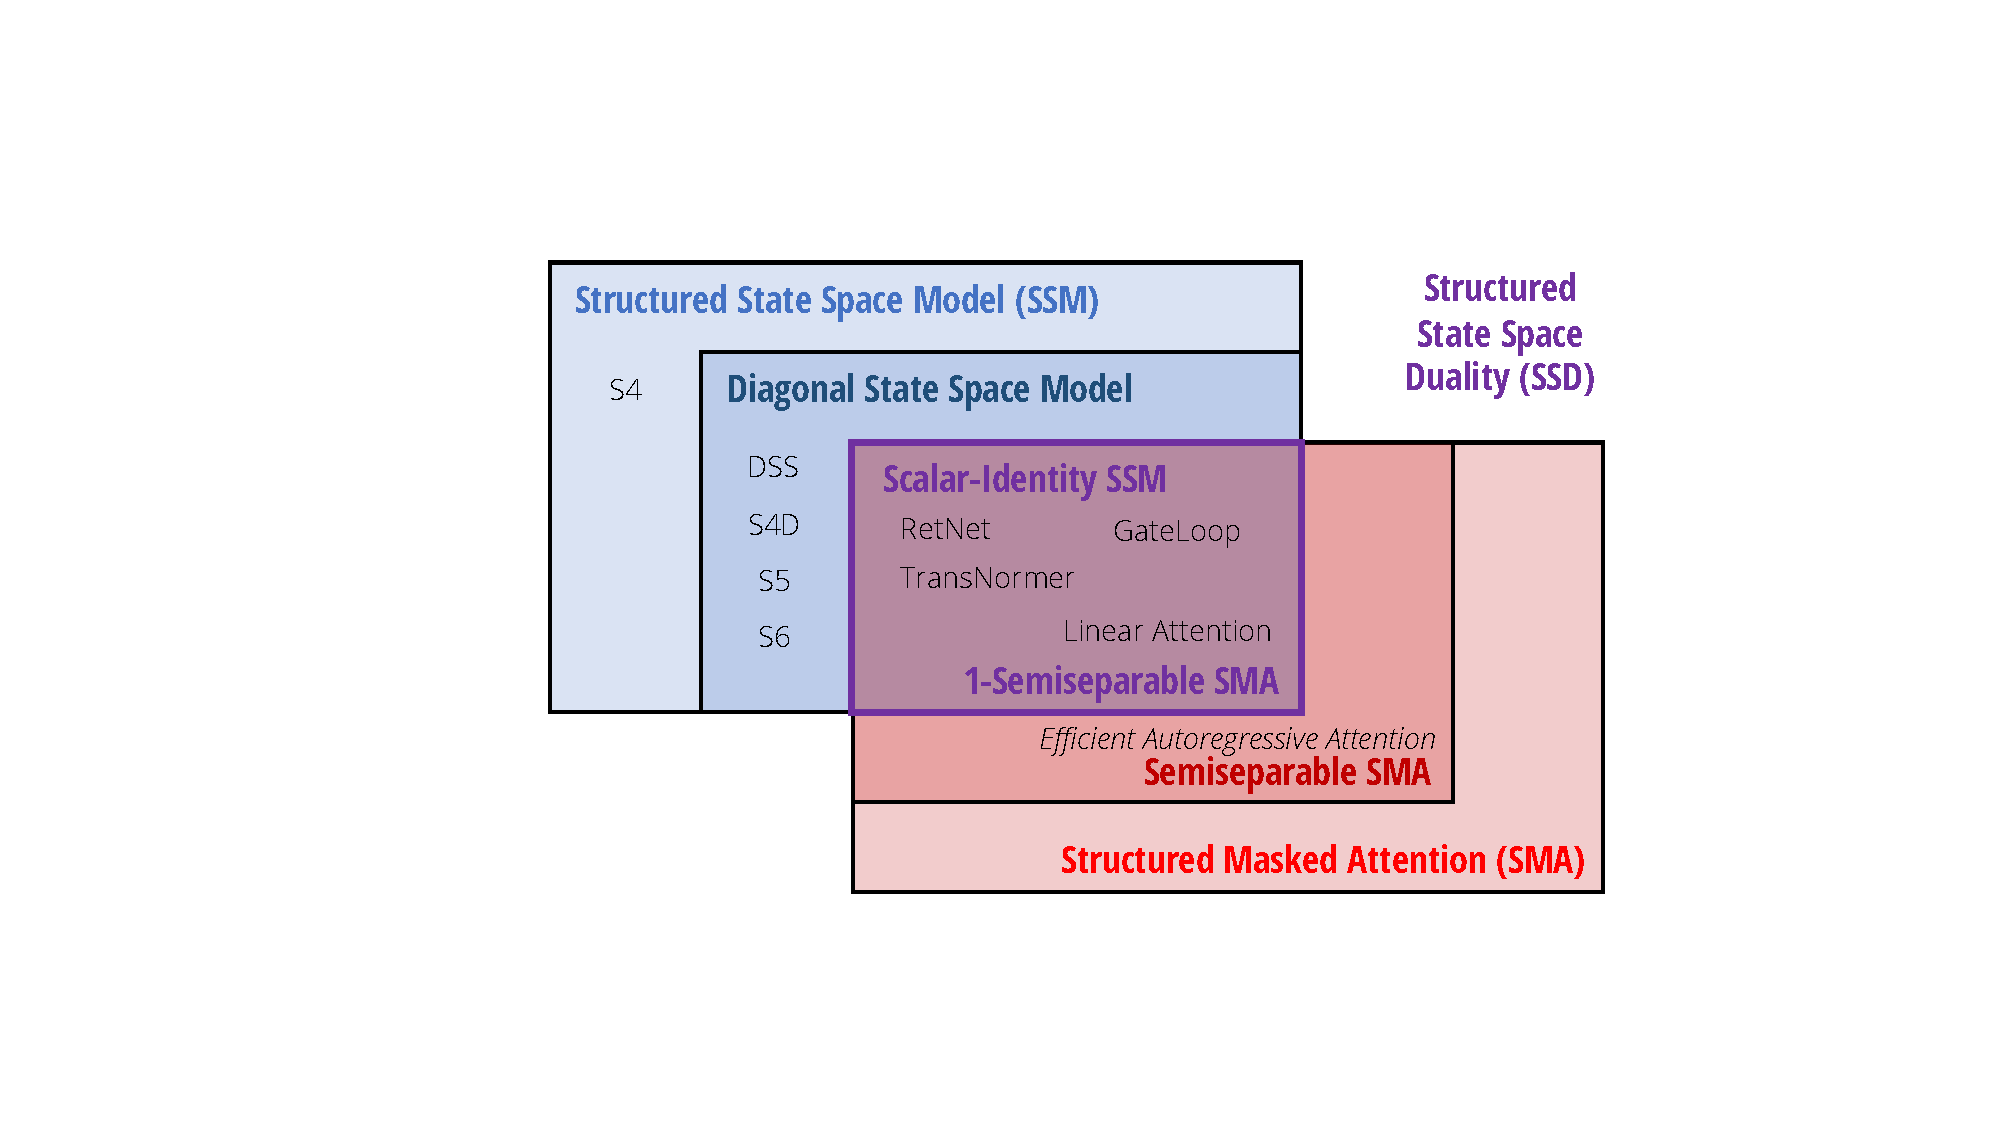
\includegraphics[width=\linewidth]{fig/ssd_venn.pdf}
  \end{minipage}
  \captionsetup{type=figure}
  \caption{
    (\textbf{Structured State Space Duality}.)
    State space duality describes the close relationship between state space models and masked attention.
    (\emph{Left}) General SSMs and SMA both possess linear and quadratic forms, with direct analogs in notation.
    (\emph{Right}) SSMs and SMA intersect at a large class of \emph{state space dual models} (SSD) which capture many sequence models as special cases.
  }
  \label{fig:ssd}
\end{figure*}

An extended related work and discussion (\cref{sec:related}) describes the relationship between SSD and general SSMs / attention in more detail.



\section{A Hardware-Efficient Algorithm for SSD Models}
\label{sec:efficient}


The benefits of developing the theoretical SSD framework between SSMs, attention, and structured matrices lies in using the connections to improve the models and algorithms.
In this section, we show how various algorithms for computing SSD models efficiently can be derived from various algorithms for computing structured matrix multiplication.

\iftoggle{arxiv}{
Our main computational result is an algorithm for computing SSD models that combines both the linear (recurrent) mode and quadratic (attention) mode.
This algorithm is as computation efficient as SSMs (linear scaling in sequence length) and as hardware-friendly as attention (primarily uses matrix multiplications).


\begin{theorem}
  \label{thm:algorithm}
  Consider an SSD model with state expansion factor $\mathtt{N}$ and head dimension $\mathtt{P}=\mathtt{N}$.
  There exists an algorithm for computing the model on any input $X \in \R^{\mathtt{(T, P)}}$
  which only requires $O(\mathtt{TN}^2)$ training FLOPs, $O(\mathtt{TN})$ inference FLOPs,
  $O(\mathtt{N}^2)$ inference memory,
  and whose work is dominated by matrix multiplications.
\end{theorem}
Note that all of these bounds are tight, because
a state space model with state expansion $\mathtt{N}$ operating on a head size of $\mathtt{N}$ has total state size $\mathtt{N}^2$ (yielding the lower bounds for training and inference FLOPs of $O(\mathtt{TN}^2)$ and $O(\mathtt{N}^2)$ respectively).
Furthermore the input $X$ itself has $\mathtt{TN}$ elements, yielding the memory lower bound.

The main idea behind \cref{thm:algorithm} is once again viewing the problem of computing a state space model as a semiseparable matrix multiplication, but leveraging its structure in a new way.
Instead of computing the whole matrix in either recurrent or attention mode,
we perform a \emph{block decomposition} of the matrix.
The diagonal blocks can be computed using the dual attention mode, which can be efficiently done with matrix multiplications,
while the off-diagonal blocks can be factored by the rank-structure of semiseparable matrices and reduced to a smaller recurrence.
We highlight that \cref{listing} provides a self-contained implementation of the SSD algorithm.
Compared to the general selective SSM of \citet{gu2023mamba},
this implementation is much simpler, and relatively efficient even in native PyTorch without requiring special low-level kernels.
}{
}




To begin, we partition the matrix $M$ into a $\frac{\mathtt{T}}{\mathtt{Q}} \times \frac{\mathtt{T}}{\mathtt{Q}}$ grid of submatrices of size $\mathtt{Q} \times \mathtt{Q}$,
for some block size $\mathtt{Q}$.
Note that the off-diagonal blocks are low-rank by the defining property of semiseparable matrices (\cref{def:semiseparable-rank}).%
\footnote{Note that the block decomposition is valid even with partitions of varying size, e.g.\ if $\mathtt{Q} \not\mid \mathtt{T}$, but we assume even divisibility for simplicity.}
\begin{align*}%
  \text{(Block Decomposition)} \quad M &=
  \begin{bmatrix}
    M^{(0,0)} \\
    M^{(1,0)} & M^{(1,1)} \\
    \vdots & \vdots & \ddots \\
    M^{(\mathtt{T}/\mathtt{Q}-1,0)} & M^{(\mathtt{T}/\mathtt{Q}-1,1)} & \dots & M^{(\mathtt{T}/\mathtt{Q}-1,\mathtt{T}/\mathtt{Q}-1)} \\
  \end{bmatrix}
  \\
  \text{(Diagonal Block)} \quad M^{(j,j)} &= \mathsf{SSM}(A_{j\mathtt{Q}:(j+1)\mathtt{Q}}, B_{j\mathtt{Q}:(j+1)\mathtt{Q}}, C_{j\mathtt{Q}:(j+1)\mathtt{Q}}) \\
  \text{(Low-Rank Block)} \quad M^{(j,i)} &= 
  \begin{bmatrix}C_{j\mathtt{Q}}^{\top} A_{j\mathtt{Q}:j\mathtt{Q}-1} \\[1pt] \vdots \\[1pt] C_{(j+1)\mathtt{Q}-1}^{\top} A_{(j+1)\mathtt{Q}-1:j\mathtt{Q}-1}\end{bmatrix}
  A_{j\mathtt{Q}-1:(i+1)\mathtt{Q}-1}
  \begin{bmatrix}B_{i\mathtt{Q}}^{\top} A_{(i+1)\mathtt{Q}-1:i\mathtt{Q}} \\[1pt] \vdots \\[1pt] B_{(i+1)\mathtt{Q}-1}^{\top} A_{(i+1)\mathtt{Q}-1:(i+1)\mathtt{Q}-1}\end{bmatrix}^{\top}
\end{align*}

This is easiest illustrated through an example, e.g.\ for $\mathtt{T}=9$ and decomposing into chunks of length $\mathtt{Q}=3$.
The shaded cells are low-rank factorizations of the off-diagonal blocks of the semiseparable matrix.
\begin{align*}%
M &=
\begin{bNiceArray}{ccc|ccc|ccc}[cell-space-limits=2pt]
    C_0^{\top} A_{0:0} B_0 & \\
    C_1^{\top} A_{1:0} B_0 & C_1^{\top} A_{1:1} B_1 & \\
    C_2^{\top} A_{2:0} B_0 & C_2^{\top} A_{2:1} B_1 & C_2^{\top} A_{2:2} B_2 \\
    \hline
    C_3^{\top} A_{3:0} B_0 & C_3^{\top} A_{3:1} B_1 & C_3^{\top} A_{3:2} B_2 & C_3^{\top} A_{3:3} B_3 \\
    C_4^{\top} A_{4:0} B_0 & C_4^{\top} A_{4:1} B_1 & C_4^{\top} A_{4:2} B_2 & C_4^{\top} A_{4:3} B_3 & C_4^{\top} A_{4:4} B_4 \\
    C_5^{\top} A_{5:0} B_0 & C_5^{\top} A_{5:1} B_1 & C_5^{\top} A_{5:2} B_2 & C_5^{\top} A_{5:3} B_3 & C_5^{\top} A_{5:4} B_4 & C_5^{\top} A_{5:5} B_5 \\
    \hline
    C_6^{\top} A_{6:0} B_0 & C_6^{\top} A_{6:1} B_1 & C_6^{\top} A_{6:2} B_2 & C_6^{\top} A_{6:3} B_3 & C_6^{\top} A_{6:4} B_4 & C_6^{\top} A_{6:5} B_5 & C_6^{\top} A_{6:6} B_6 \\
    C_7^{\top} A_{7:0} B_0 & C_7^{\top} A_{7:1} B_1 & C_7^{\top} A_{7:2} B_2 & C_7^{\top} A_{7:3} B_3 & C_7^{\top} A_{7:4} B_4 & C_7^{\top} A_{7:5} B_5 & C_7^{\top} A_{7:6} B_6 & C_7^{\top} A_{7:7} B_7 \\
    C_8^{\top} A_{8:0} B_0 & C_8^{\top} A_{8:1} B_1 & C_8^{\top} A_{8:2} B_2 & C_8^{\top} A_{8:3} B_3 & C_8^{\top} A_{8:4} B_4 & C_8^{\top} A_{8:5} B_5 & C_8^{\top} A_{8:6} B_6 & C_8^{\top} A_{8:7} B_7 & C_8^{\top} A_{8:8} B_8 \\
\end{bNiceArray}
\\
\\&=
\begin{bNiceArray}{ccc|ccc|ccc}[cell-space-limits=2pt]
    C_0^{\top} A_{0:0} B_0 & \\
    C_1^{\top} A_{1:0} B_0 & C_1^{\top} A_{1:1} B_1 & \\
    C_2^{\top} A_{2:0} B_0 & C_2^{\top} A_{2:1} B_1 & C_2^{\top} A_{2:2} B_2 \\
    \hline
    \Block[fill=[RGB]{243,240,255}]{3-3}{\begin{bmatrix}C_3^{\top} A_{3:2} \\[1pt] C_4^{\top} A_{4:2} \\[1pt] C_5^{\top} A_{5:2}\end{bmatrix}A_{2:2}\begin{bmatrix}B_0^{\top} A_{2:0} \\[1pt] B_1^{\top} A_{2:1} \\[1pt] B_2^{\top} A_{2:2}\end{bmatrix}^{\top}}
                           &&& C_3^{\top} A_{3:3} B_3 \\
                           &&& C_4^{\top} A_{4:3} B_3 & C_4^{\top} A_{4:4} B_4 \\
                           &&& C_5^{\top} A_{5:3} B_3 & C_5^{\top} A_{5:4} B_4 & C_5^{\top} A_{5:5} B_5 \\
    \hline
    \Block[fill=[RGB]{243,240,255}]{3-3}{\begin{bmatrix}C_6^{\top} A_{6:5} \\[1pt] C_7^{\top} A_{7:5} \\[1pt] C_8^{\top} A_{8:5}\end{bmatrix}A_{5:2}\begin{bmatrix}B_0^{\top} A_{2:0} \\[1pt] B_1^{\top}A_{2:1} \\[1pt] B_2^{\top}A_{2:2}\end{bmatrix}^{\top}}
                           &&&
                           \Block[fill=[RGB]{243,240,255}]{3-3}{\begin{bmatrix}C_6^{\top} A_{6:5} \\[1pt] C_7^{\top} A_{7:5} \\[1pt] C_8^{\top} A_{8:5}\end{bmatrix}A_{5:5}\begin{bmatrix}B_3^{\top}A_{5:3} \\[1pt] B_4^{\top}A_{5:4} \\[1pt] B_5^{\top}A_{5:5}\end{bmatrix}^{\top}}
                           &&& C_6^{\top} A_{6:6} B_6 \\
                           &&&&&& C_7^{\top} A_{7:6} B_6 & C_7^{\top} A_{7:7} B_7 \\
                           &&&&&& C_8^{\top} A_{8:6} B_6 & C_8^{\top} A_{8:7} B_7 & C_8^{\top} A_{8:8} B_8 \\
  \end{bNiceArray}
\end{align*}

From here we can reduce the problem into these two parts.
These can also be interpreted as dividing the output of a ``chunk'' $y_{j\mathtt{Q}:(j+1)\mathtt{Q}}$ into two components:
the effect of inputs within the chunk $x_{j\mathtt{Q}:(j+1)\mathtt{Q}}$, and the effect of inputs before the chunk $x_{0:j\mathtt{Q}}$.

\subsection{Diagonal Blocks}
The diagonal blocks are easy to handle, because they are simply self-similar problems of a smaller size.
The $j$-th block represents computing the answer $\mathsf{SSM}(A_R, B_R, C_R)(x_R)$ for the range $R = j\mathtt{Q}:(j+1)\mathtt{Q} = (j\mathtt{Q}, j\mathtt{Q}+1, \dots, j\mathtt{Q}+\mathtt{Q}-1)$.
The key is that this block can be computed using any desired method.
In particular, for small chunk lengths $\mathtt{Q}$, this problem is computed more efficiently using the dual quadratic SMA form.
Additionally, the chunks can be computed in parallel.

These subproblems can be interpreted as: what is the output per chunk \emph{supposing that the initial state (to the chunk) is $0$}.
In other words for chunk $j$, this computes the correct outputs taking into account only the chunk inputs $x_{j\mathtt{Q}:(j+1)\mathtt{Q}}$.

\subsection{Low-Rank Blocks}

The low-rank factorizations consist of 3 terms, and there are correspondingly three pieces of the computation.
In this factorization, we will use the terminology
\begin{itemize}
  \item The terms like $\begin{bmatrix}B_0^{\top} A_{2:0} \\[1pt] B_1^{\top}A_{2:1} \\[1pt] B_2^{\top}A_{2:2}\end{bmatrix}^{\top}$ are called the right factors or $B$-block-factors.
  \item The terms like $A_{5:2}$ are called the center factors or $A$-block-factors.
  \item The terms like $\begin{bmatrix}C_6^{\top} A_{6:5} \\[1pt] C_7^{\top} A_{7:5} \\[1pt] C_8^{\top} A_{8:5}\end{bmatrix}$ are called the left factors or $C$-block-factors.
\end{itemize}


\paragraph{Right Factors.}

This step computes the multiplication by the right $B$-block-factors of the low-rank factorization.
Note that for each chunk, this is a $(\mathtt{N}, \mathtt{Q})$ by $(\mathtt{Q}, \mathtt{P})$ matrix multiplication, where $\mathtt{N}$ is the state dimension and $P$ is the head dimension.
The result is a $(\mathtt{N}, \mathtt{P})$ tensor for each chunk, which has the same dimensionality as the expanded hidden state $h$.

This can be interpreted as: what is the final state per chunk \emph{supposing that the initial state (to the chunk) is $0$}.
In other words this computes $h_{j\mathtt{Q}+\mathtt{Q}-1}$ assuming that $x_{0:j\mathtt{Q}} = 0$.

\paragraph{Center Factors.}

This step computes the effect of the center $A$-block-factors terms in the low-rank factorization.
In the previous step, the final states per chunk have total shape $\mathtt{(\mathtt{T}/\mathtt{Q},\mathtt{N},\mathtt{P})}$.
This is now multiplied by a 1-SS matrix generated by $A_{2\mathtt{Q}-1:\mathtt{Q}-1}^\times, A_{3\mathtt{Q}-1:2\mathtt{Q}-1}^\times, \dots, A_{\mathtt{T}-1:\mathtt{T}-\mathtt{Q}-1}^\times$.

This step can be computed by any algorithm for computing 1-SS multiplication (also known as the scalar SSM scan or \texttt{cumprodsum} operator).

This can be interpreted as: what is the actual final state per chunk \emph{taking into account all previous inputs};
in other words, this computes the true hidden state $h_{j\mathtt{Q}}$ taking into account all of $x_{0:(j+1)\mathtt{Q}}$.

\paragraph{Left Factors.}

This step computes the multiplication by the left $C$-block-factors of the low-rank factorization.
For each chunk, this can be represented by a matrix multiplication
$\mathsf{contract}(\mathtt{QN,NP \to QP})$.

This can be interpreted as: what is the output per chunk \emph{taking into account the correct initial state $h_{j\mathtt{Q}-1}$, and supposing the inputs $x_{j\mathtt{Q}:(j+1)\mathtt{Q}}$ are $0$}.
In other words for chunk $j$, this computes the correct outputs taking into account only the prior inputs $x_{0:j\mathtt{Q}}$.

\begin{listing*}[!t]
\inputminted[fontsize=\footnotesize]{python}{structure/code.py}
\caption{Full PyTorch example of the state space dual (SSD) model.}
\label{listing}
\end{listing*}


\begin{figure}[!t]
\centering
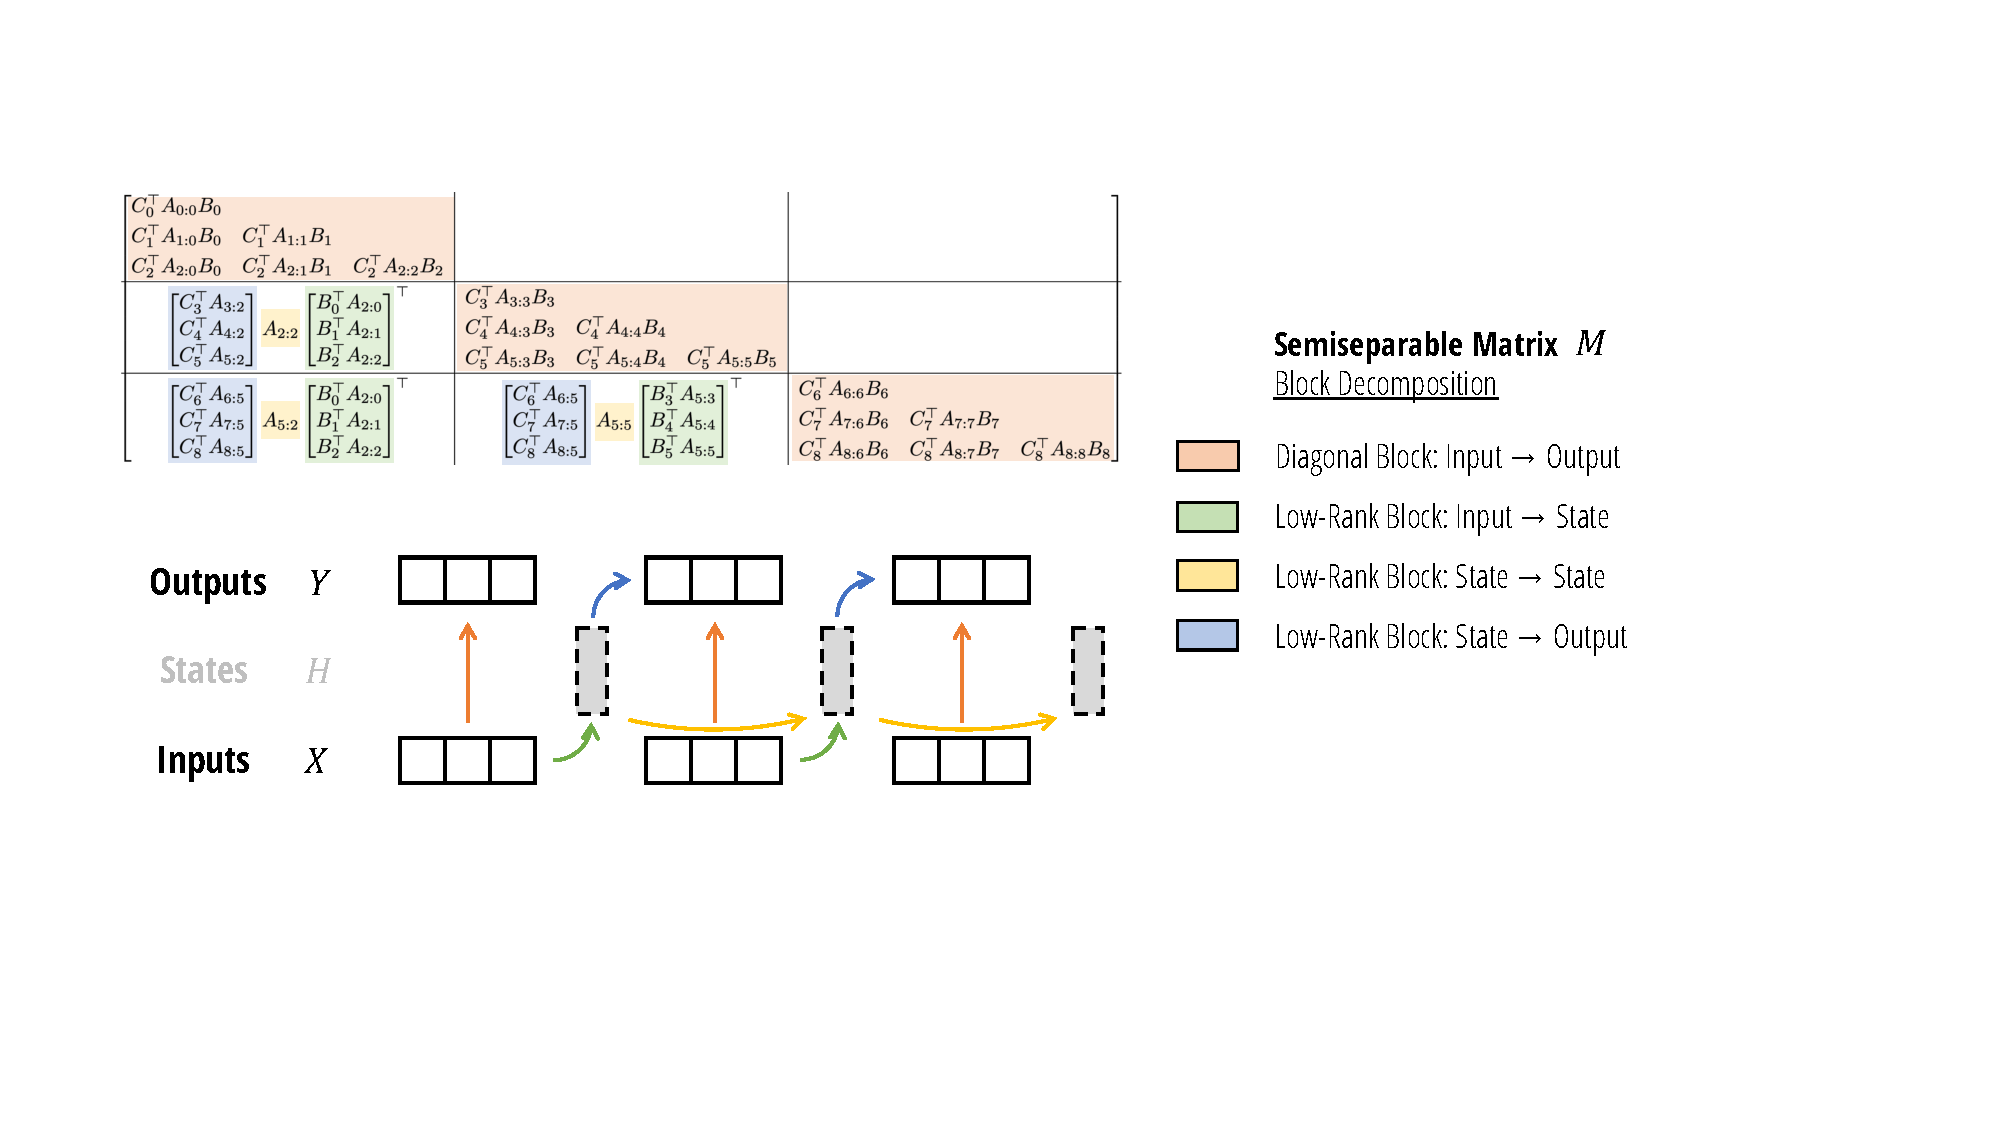
\includegraphics[width=\linewidth]{fig/ssd_algorithm.pdf}
\caption{
  (\textbf{SSD Algorithm}.)
  By using the matrix transformation viewpoint of state space models to write them as semiseparable matrices (\cref{sec:ssm}), we develop a more hardware-efficient computation of the SSD model through a block-decomposition matrix multiplication algorithm.
  The matrix multiplication also has an interpretation as a state space model,
  where blocks represent chunking the input and output sequence.
  Diagonal blocks represent intra-chunk computations and the off-diagonal blocks represent inter-chunk computations, factored through the SSM's hidden state.
}
\label{fig:ssd-algorithm}
\end{figure}

\subsection{Computational Cost}

We define the notation $\mathsf{BMM}(\mathtt{B}, \mathtt{M}, \mathtt{N}, \mathtt{K})$ to define a batched matrix multiplication $\mathsf{contract}(\mathtt{\mathtt{MK},\mathtt{KN} \to \mathtt{MN}})$ with batch dimension $\mathtt{B}$.
From this notation we can infer three aspects of the efficiency:
\begin{itemize}
  \item \emph{Computation cost}: total of $O(\mathtt{BMNK})$ FLOPs.
  \item \emph{Memory cost:} total of $O(\mathtt{B}(\mathtt{MK}+\mathtt{KN}+\mathtt{MN}))$ space.
  \item \emph{Parallelization:} larger $\mathtt{M}, \mathtt{N}, \mathtt{K}$ terms can leverage specialized matrix multiplication units on modern accelerators.
\end{itemize}

\paragraph{Center Blocks.}
The cost of the quadratic SMA computation consists of three steps (equation \eqref{eq:ssm-quad}):
\begin{itemize}
  \item Computing the kernel matrix $C^{\top} B$, which has cost $\mathsf{BMM}(\mathtt{T}/\mathtt{Q}, \mathtt{Q}, \mathtt{Q}, \mathtt{N})$.
  \item Multiplying by the mask matrix, which is an elementwise operation on tensors of shape $(\mathtt{T}/\mathtt{Q}, \mathtt{Q}, \mathtt{Q})$.
  \item Multiplying by the $X$ values, which has cost $\mathsf{BMM}(\mathtt{T}/\mathtt{Q}, \mathtt{Q}, \mathtt{P}, \mathtt{N})$
\end{itemize}

\paragraph{Low-Rank Blocks: Right Factors.}
This step is a single matrix multiplication with cost $\mathsf{BMM}(\mathtt{T}/\mathtt{Q}, \mathtt{N}, \mathtt{P}, \mathtt{Q})$.

\paragraph{Low-Rank Blocks: Center Factors.}
This step is a scalar SSM scan (or 1-SS multiplication) of length $\mathtt{T}/\mathtt{Q}$ on $(\mathtt{N}, \mathtt{P})$ independent channels.
The work of this scan is $\mathtt{TNP}/\mathtt{Q}$, which is negligible compared to the other factors.

Note that because of the blocking which reduces the length of the sequence from $\mathtt{T}$ to $\mathtt{T}/\mathtt{Q}$,
this scan has $\mathtt{Q}$ times smaller cost than a pure SSM scan (e.g. the selective scan of Mamba).
Thus we observe that on most problem lengths,
other algorithms (\cref{sec:scan}) may be more efficient or much easier to implement without a significant slowdown.
For example, a naive implementation of this via 1-SS matrix multiplication has cost $\mathsf{BMM}(1, \mathtt{T}/\mathtt{Q}, \mathtt{NP}, \mathtt{T}/\mathtt{Q})$,
which is much easier to implement and can be more efficient than a naive recurrence/scan implementation.

\paragraph{Low-Rank Blocks: Left Factors.}
This step is a single matrix multiplication with cost $\mathsf{BMM}(\mathtt{T}/\mathtt{Q}, \mathtt{Q}, \mathtt{P}, \mathtt{N})$.

\paragraph{Total Cost.}
If we set $\mathtt{N} = \mathtt{P} = \mathtt{Q}$ (in other words the state dimension, head dimension, and chunk length are equal),
then all BMM terms above become $\mathsf{BMM}(\mathtt{T}/\mathtt{N}, \mathtt{N}, \mathtt{N}, \mathtt{N})$.
The computational chacteristics of this are:
\begin{itemize}
  \item Total FLOP count of $O(\mathtt{TN}^2)$.
  \item Total memory of $O(\mathtt{TN})$.
  \item The work \emph{consists primarily of matrix multiplications} on matrices of shape $(\mathtt{N}, \mathtt{N})$.
\end{itemize}
Notice that the memory consumption is tight; the inputs and outputs $x, y$ have shape $(\mathtt{T}, \mathtt{P}) = (\mathtt{T}, \mathtt{N})$.
Meanwhile the flop count reflects an extra factor of $\mathtt{N}$, which is cost incurred by the autoregressive state size and is common to all models.

Aside from the matmuls, there is a scalar SSM scan on $\mathtt{NP} = \mathtt{N}^2$ features and sequence length $\mathtt{T}/\mathtt{Q}$.
This has cost $O(\mathtt{T}/\mathtt{Q} \mathtt{N}^2)$ FLOPs and $O(\log(\mathtt{T}/\mathtt{Q}))$ depth.
Although it does not use matrix multiplications, it is still parallelizable and the total work done is negligible compared to the other steps;
this has a negligible cost in our GPU implementation.

\paragraph{Comparison to Pure SSM and Attention Models.}

Quadratic attention is also very hardware efficient by only leveraging matrix multiplications, but has $\mathtt{T}^2 N$ total FLOPs.
Its slower computation speed at both training and inference can directly be seen as a consequence of having a larger state size -- standard attention has a state size scaling with sequence length $\mathtt{T}$ because it caches its history and does not compress its state.

Linear SSMs have $\mathtt{TNP} = \mathtt{TN}^2$ total FLOPs, which is the same as SSD.
However, a naive implementation requires a state expansion \eqref{eq:sha-lin:1} that materializes extra memory,
and a scalar operation \eqref{eq:sha-lin:2} that does not leverage matrix multiplications.


\begin{center}
  \begin{tabular}{@{}llll@{}}
    \toprule
                            & Attention                & SSM                                        & \textbf{SSD} \\
    \midrule
    State size              & $\mathtt{T}$             & $\mathtt{\mathbf{N}}$                      & $\mathtt{\mathbf{N}}$ \\
    Training FLOPs          & $\mathtt{T}^2\mathtt{N}$ & $\mathtt{\mathbf{T}}\mathtt{\mathbf{N}}^2$ & $\mathtt{\mathbf{T}}\mathtt{\mathbf{N}}^2$ \\
    Inference FLOPs         & $\mathtt{T}\mathtt{N}$   & $\mathtt{\mathbf{N}}^2$                    & $\mathtt{\mathbf{N}}^2$ \\
    \midrule
    (Naive) memory          & $\mathtt{T}^2$           & $\mathtt{T}\mathtt{N}^2$                   & $\mathtt{\mathbf{T}}\mathtt{\mathbf{N}}$ \\
    Matrix multiplication   & \cmark                   &                                            & \textbf{\cmark} \\
    \bottomrule
  \end{tabular}
  \label{tab:compute}
\end{center}

We note that many other matrix decompositions are possible (for example, see \cref{sec:scan} for a compendium of algorithms for 1-SS multiplication through different structured matrix decompositions)
which may lead to more algorithms for SSDs that could be better for other specialized settings.
Even more broadly, we note that semiseparable matrices have a rich literature and many more representations besides the SSS form that we use (\cref{def:sss}),
and even more efficient algorithms may be possible.

\section{The Mamba-2 Architecture}
\label{sec:architecture}

By connecting SSMs and attention, the SSD framework allows us to develop a shared vocabulary and library of techniques for both.
In this section we discuss some examples of understanding and modifying SSD layers using ideas originally developed for Transformers.
We discuss several design choices, resulting in the Mamba-2 architecture.
These axes of variation are ablated in \cref{sec:experiments:ablations}.


\begin{figure}[!t]
  \centering
  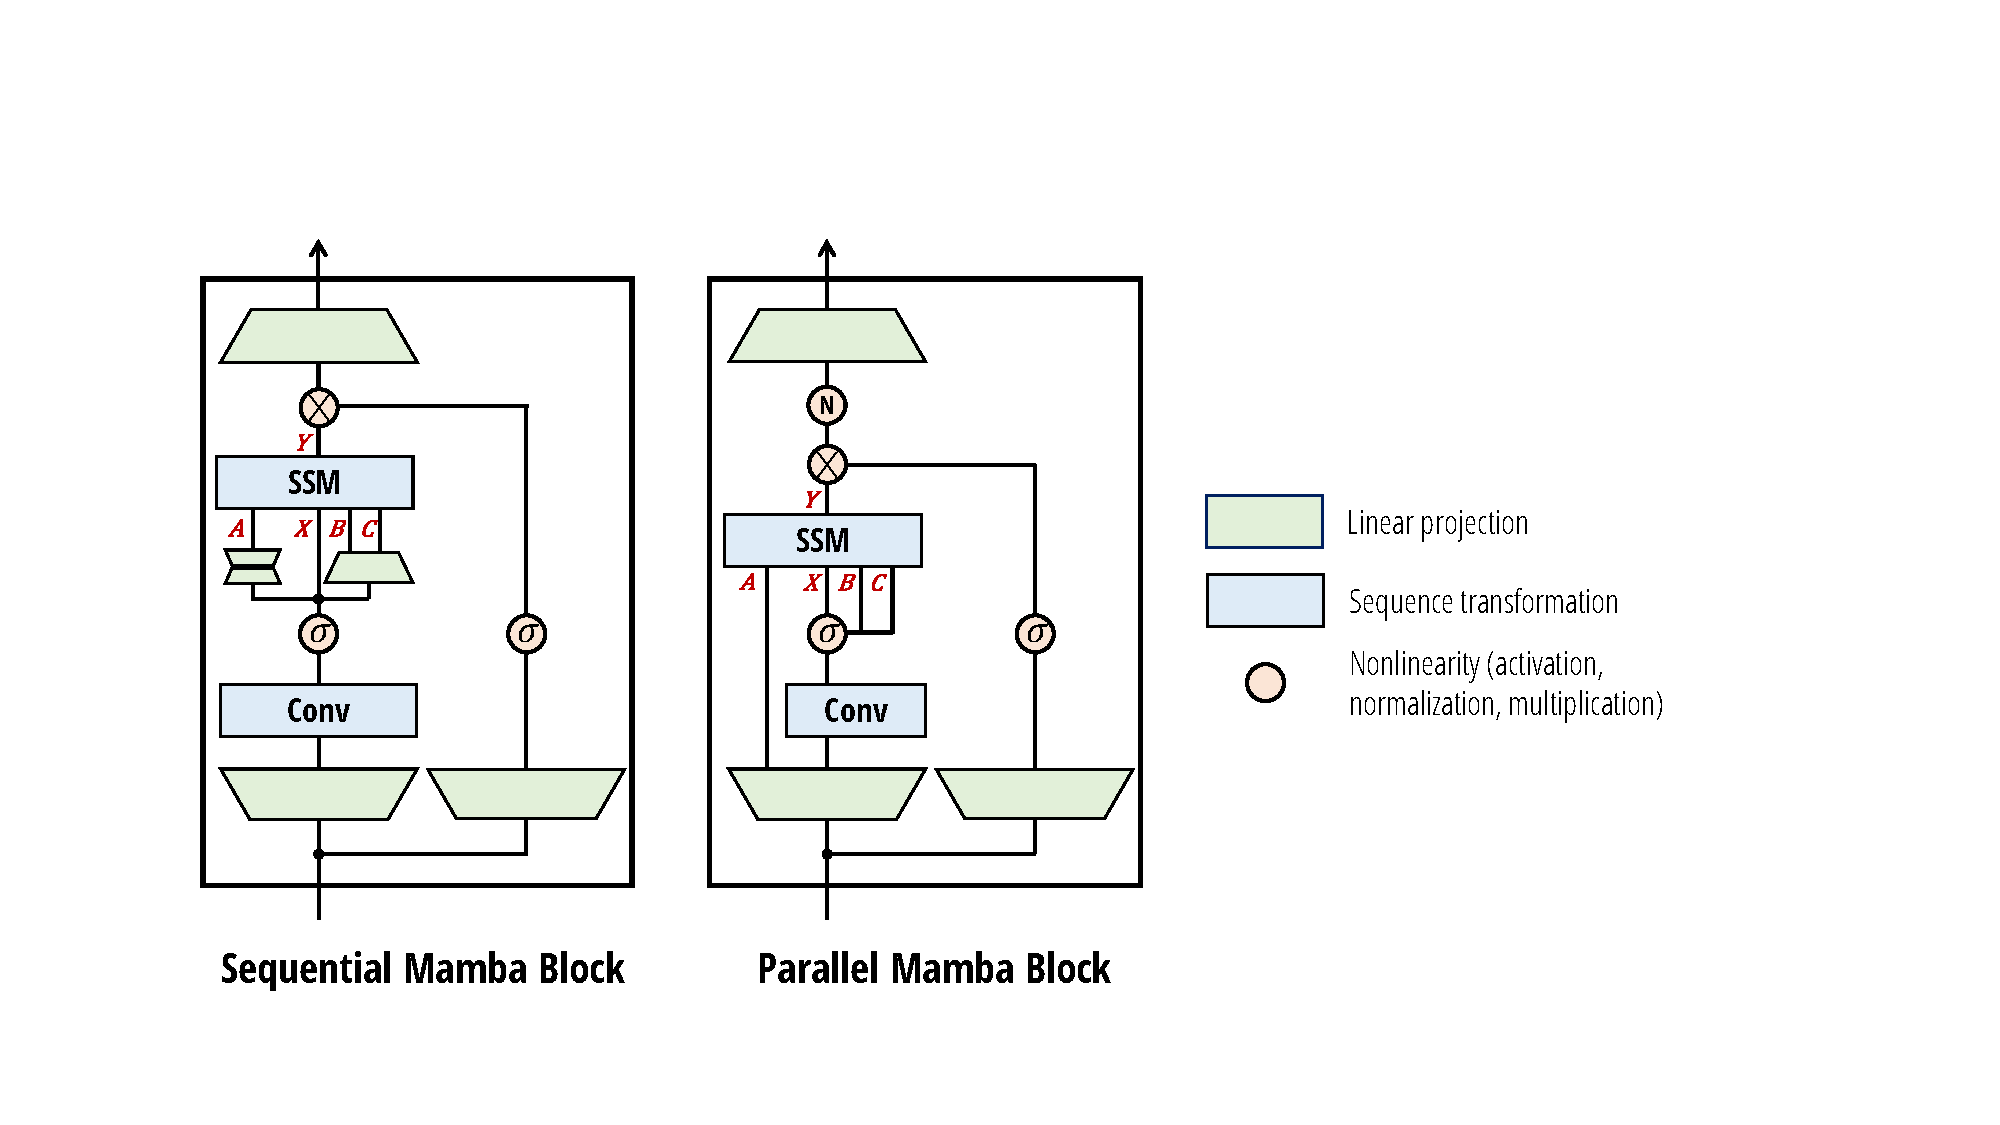
\includegraphics[width=\iftoggle{arxiv}{0.8\linewidth}{\linewidth}]{fig/architecture_2.pdf}
  \caption{
    (\textbf{Mamba-2 Architecture}.) The Mamba-2 block simplifies the Mamba block by removing sequential linear projections; the SSM parameters $A, B, C$ are produced at the beginning of the block instead of as a function of the SSM input $X$.
    An additional normalization layer is added as in NormFormer~\citep{shleifer2021normformer}, improving stability.
    The $B$ and $C$ projections only have a single head shared across the $X$ heads, analogous to multi-value attention (MVA).
  }
  \label{fig:architecture}
  \iftoggle{arxiv}{}{\vspace{-1.25em}}
\end{figure}

\subsection{Block Design}
\label{sec:architecture:block}


We first discuss modifications to the neural network block that are independent of the inner sequence mixing layer (i.e. outside the core SSD layer).

\paragraph{Parallel Parameter Projections.}

Mamba-1 was motivated by an SSM-centric point of view
where the selective SSM layer is viewed as a map from $X \mapsto Y$.
The SSM parameters $A, B, C$ are viewed as
subsidiary and are functions of the SSM input $X$.
Thus the linear projections defining $(A, B, C)$ occur after the initial linear projection to create $X$.

In Mamba-2, the SSD layer is viewed as a map from $A, X, B, C \mapsto Y$.
It therefore makes sense to produce $A, X, B, C$ in parallel with a single projection at the beginning of the block.
Note the analogy to standard attention architectures,
where $X, B, C$ correspond to the $Q, K, V$ projections that are created in parallel.

Note that adopting parallel projections for the $A, B, C, X$ inputs to the SSM slightly reduces parameters and more importantly is more amenable to tensor parallelism for larger models, by using standard Megatron sharding patterns~\citep{shoeybi2019megatron}).


\paragraph{Extra Normalization.}

In preliminary experiments, we found that instabilities were prone to arising in larger models.
We were able to alleviate this by adding an extra normalization layer (e.g. LayerNorm, GroupNorm, or RMSNorm) to the block right before the final output projection.
This usage of a normalization is most directly related to the NormFormer architecture~\citep{shleifer2021normformer}, which also added normalization layers at the end of the MLP and MHA blocks.

We also note that this change is similar to other recent models related to Mamba-2 that were derived from a linear attention viewpoint.
The original linear attention formulation normalizes by a denominator term that emulates the normalization of the softmax function in standard attention.
TransNormerLLM~\citep{qin2023transnormerllm} and RetNet~\citep{sun2023retentive} find that this normalization is unstable and add an extra LayerNorm or GroupNorm after the linear attention layer.
Our extra normalization layer differs slightly from these, occuring after the multiplicative gate branch instead of before.


\subsection{Multihead Patterns for Sequence Transformations}
\label{sec:architecture:multihead}

Recall that SSMs are defined as a sequence transformation (\cref{def:sequence-transformation})
where:
\begin{itemize}
  \item $A, B, C$ parameters have a state dimension $\mathtt{N}$.
  \item They define a sequence transformation $\R^\mathtt{T} \to \R^\mathtt{T}$, which for example can be represented as a matrix $M \in \R^{\mathtt{(T, T)}}$.
  \item This transformation operates over an input sequence $X \in \R^{\mathtt{(T, P)}}$, independently over the $\mathtt{P}$ axis.
\end{itemize}
One can view this as defining one \emph{head} of the sequence transformation.
\begin{definition}[Multihead patterns]
  \label{def:head-pattern}
  A multihead sequence transformation consists of $\mathtt{H}$ independent heads, for a total model dimension of $\mathtt{D}=\mathtt{d\_model}$.
  The parameters may be tied across heads, leading to a \textbf{head pattern}.
\end{definition}
The state size $\mathtt{N}$ and head dimension $\mathtt{P}$ are analogous to the $QK$ head dimension and $V$ head dimension of attention, respectively.
Just as in modern Transformer architectures~\citep{chowdhery2022palm,touvron2023llama},
in Mamba-2 we generally choose these to be constants around $64$ or $128$; when the model dimension $\mathtt{D}$ increases, we increase the number of heads while keeping the head dimensions $\mathtt{N}$ and $\mathtt{P}$ fixed.
In order to describe how to do this,
we can transfer and generalize ideas from multihead attention to define similar patterns for SSMs, or any general sequence transformation.

\begin{minipage}[t]{.25\linewidth}
  \begin{equation}%
    \label{eq:multihead}
    \begin{aligned}%
        & \textbf{Multi-head SSM} \\
        & (\textrm{Multi-head Attn.}) \\
      X & \quad \mathtt{(T, H, P)} \\
      A & \quad \mathtt{(T, H)} \\
      B & \quad \mathtt{(T, H, N)} \\
      C & \quad \mathtt{(T, H, N)} \\
    \end{aligned}
  \end{equation}
\end{minipage}
\begin{minipage}[t]{.25\linewidth}
  \begin{equation}%
    \label{eq:multiquery}
    \begin{aligned}%
    & \textbf{Multi-contract SSM} \\
    & (\textrm{Multi-query Attn.}) \\
      X & \quad \mathtt{(T, 1, P)} \\
      A & \quad \mathtt{(T, H)} \\
      B & \quad \mathtt{(T, 1, N)} \\
      C & \quad \mathtt{(T, H, N)} \\
    \end{aligned}
  \end{equation}
\end{minipage}
\begin{minipage}[t]{.25\linewidth}
  \begin{equation}%
    \label{eq:multikey}
    \begin{aligned}%
    & \textbf{Multi-expand SSM} \\
    & (\textrm{Multi-key Attn.}) \\
      X & \quad \mathtt{(T, 1, P)} \\
      A & \quad \mathtt{(T, H)} \\
      B & \quad \mathtt{(T, H, N)} \\
      C & \quad \mathtt{(T, 1, N)} \\
    \end{aligned}
  \end{equation}
\end{minipage}
\begin{minipage}[t]{.25\linewidth}
  \begin{equation}%
    \label{eq:multivalue}
    \begin{aligned}%
    & \textbf{Multi-input SSM} \\
    & (\textrm{Multi-value Attn.}) \\
      X & \quad \mathtt{(T, H, P)} \\
      A & \quad \mathtt{(T, H)} \\
      B & \quad \mathtt{(T, 1, N)} \\
      C & \quad \mathtt{(T, 1, N)} \\
    \end{aligned}
  \end{equation}
\end{minipage}

\paragraph{Multihead SSM (MHS) / Multihead Attention (MHA) Pattern.}

The classic MHA pattern assumes that the head dimension $\mathtt{P}$ divides the model dimension $\mathtt{D}$.
The number of heads is defined as $\mathtt{H} = \mathtt{D} / \mathtt{P}$.
Then, $\mathtt{H}$ copies of the core sequence transformation are created by creating $\mathtt{H}$ independent copies of each parameter.
Note that while the MHA pattern was first described for the attention sequence transformation,
it can be applied to anything compatible with \cref{def:sequence-transformation}.
For example, a multi-head SSD layer would accept inputs with shapes according to equation \eqref{eq:multihead}
where the SSD algorithm is broadcasted over the $\mathtt{H} = \mathtt{n\_heads}$ dimension.

%

\paragraph{Multi-contract SSM (MCS) / Multi-query Attention (MQA) Pattern.}

Multi-query attention~\citep{shazeer2019fast} is a clever optimization for attention that can dramatically improve the speed of autoregressive inference,
which relies on caching the $K$ and $V$ tensors.
This technique simply avoids giving $K$ and $V$ the extra head dimension,
or in other words broadcasts a single head of $(K, V)$ across all the heads of $Q$.

Using the state space duality, we can define an equivalent SSM version of MQA as equation \eqref{eq:multiquery}.
Here, $X$ and $B$ (the SSM analogs of attention's $V$ and $K$) are shared across the $\mathtt{H}$ heads.
We also call this the \emph{multi-contract SSM (MCS)} head pattern, because the $C$ parameter which controls the SSM state contraction has independent copies per head.

We can similarly define a multi-key attention (MKA) or \emph{multi-expand SSM (MES)} head pattern,
where $B$ (which controls the SSM expansion) is independent per head while $C$ and $X$ are shared across heads.

\paragraph{Multi-input SSM (MIS) / Multi-value Attention (MVA) Pattern.}

While MQA makes sense for attention because of its KV cache, it is not the natural choice for SSMs.
In Mamba, instead, $X$ is viewed as the main input to the SSM,
and therefore $B$ and $C$ are parameters that are shared across the input channels.
We define a new multi-value attention (MVA) of \emph{multi-input SSM (MIS)} pattern in equation \eqref{eq:multivalue}, which can again be applied to any sequence transformation such as SSD.

Armed with this vocabulary, we can characterize the original Mamba architecture more precisely.
\begin{proposition}
  \label{prop:mamba-multihead}
  The selective SSM (S6) layer of the Mamba architecture~\citep{gu2023mamba} can be viewed as having
  \begin{itemize}
    \item Head dimension $P=1$: every channel has independent SSM dynamics $A$.
    \item \emph{Multi-input SSM} (MIS) or \emph{multi-value attention} (MVA) head structure: the $B, C$ matrices (corresponding to $K, Q$ in the attention duality) are shared across all channels of the input $X$ (corresponding to $V$ in attention).
  \end{itemize}
\end{proposition}

We can also ablate these head pattern variants when applied to SSD (\cref{sec:experiments:ablations:kernels}).
Interestingly, despite being controlled in parameter counts and total state dimension,
there is a noticeable difference in downstream performance.
We empirically find that the MVA pattern as originally used in Mamba performs best.

\paragraph{Grouped Head Patterns.}

The ideas of multi-query attention can be extended to \emph{grouped-query attention}~\citep{ainslie2023gqa}: instead of $1$ K and V head, one can create $\mathtt{G}$ independent K and V heads, where $1 < \mathtt{G}$ and $\mathtt{G}$ divides $\mathtt{H}$.
This is motivated both by bridging the performance difference between multi-query and multi-head attention,
and enabling more efficient tensor parallelism by setting $\mathtt{G}$ to be a multiple of the number of shards (\cref{sec:systems}).

Similarly, the multi-input SSM head pattern used in Mamba-2 can be easily extended to \textbf{grouped-input SSM (GIS)}, or synonymously \textbf{grouped-value attention (GVA)}.
The generalization is straightforward and we omit the details for simplicity.


\subsection{Other SSD Extensions from Linear Attention}
\label{sec:architecture:kernels}

We describe here an example of architectural modifications to SSD motivated by linear attention.
We ablate these in \cref{sec:experiments:ablations:kernels} as a form of negative result,
finding that they do not significantly improve performance enough to adopt them as default settings.
Nonetheless, these illustrate how the vast literature on attention can be incorporated to
define variants of SSD.
We treat the choice of kernel feature map as a hyperparameter in the Mamba-2 architecture,
and expect other simple modifications inspired by attention to be possible as well.

\paragraph{Kernel Attention Approximations to Softmax Attention.}
Many variants of linear attention or kernel attention are motivated by viewing the attention scores $\mathsf{softmax}(QK^{\top})$ as composed of
\begin{enumerate}
  \item An exponential kernel $Z = \exp(QK^{\top})$, which can be approximated by $Z = \psi(Q)\psi(K)^{\top}$ for some kernel feature map.
  \item Normalizing the kernel so that rows sum to $1$ via $M = G / G \bm{1} \bm{1}^{\top}$, where the division happens elementwise and $\bm{1}$ is the all 1's vector.
\end{enumerate}

\paragraph{Exponential Kernel Feature Maps.}

In Mamba-2, we incorporate a flexible kernel feature map, and apply it to the $B$ and $C$ branches (corresponding to the $K$ and $V$ branches in attention).
The feature map can also be optionally applied to the $X$ ($V$) branch, for simplicity and symmetry.
This is represented in \cref{fig:architecture} by an arbitrary nonlinearity.
By default, we simply choose $\psi$ to be an elementwise Swish / SiLU function~\citep{hendrycks2016gaussian,ramachandran2017swish}.
We explore other options in the ablations in \cref{sec:experiments:ablations:kernels},
including feature maps used by Linear Attention, Performer, Random Feature Attention, and cosFormer (\cref{sec:attention:kernel}).

\paragraph{Incorporating a Normalization (Denominator) Term.}

To find the denominator term, we simply have to compute $M \bm{1}$.
But recall that the final output of the model is just $Y = MX$ (equation \eqref{eq:ssm-quad}).
So the normalization terms can be found
simply by augmenting $X$ with an extra column $\bm{1}$, resulting in a tensor of shape $\mathtt{(T, P+1)}$.

Note that in this case, the kernel feature map $\psi$ must be positive so that the sum is positive.

\section{Systems Optimization for SSMs}
\label{sec:systems}

We describe several systems optimizations for SSMs, in particular the Mamba-2 architecture, for large-scale efficient training and inference.
In particular, we focus on tensor parallel and sequence parallel for large-scale training, as a well variable-length sequences for efficient finetuning and inference.

\subsection{Tensor Parallel}
\label{subsec:tp}

Tensor parallelism (TP)~\citep{shoeybi2019megatron} is a model parallelism technique that splits each layer (e.g., attention, MLP) to run on multiple accelerators such as GPUs.
This technique is widely used to train most large models~\citep{brown2020language, chowdhery2022palm, touvron2023llama, touvron2023llama2}  on GPU clusters where each node typically has 4-8 GPUs with fast networking such as NVLink.
TP was originally developed for the Transformer architecture, and it is not straight-forward to adapt it other architecture.
We first show the challenge of using TP with the Mamba architecture, and the show how the Mamba-2 architecture is designed to make TP efficient.

Recall the Mamba architecture, with a single input $u \in \mathbb{R}^{L \times d}$ (no batching for simplicity), input projection matrices $W^{(x)}, W^{(z)} \in \mathbb{R}^{d \times ed}$ where $e$ is the expansion factor (typically 2), and output projection matrix $W^{(o)} \in \mathbb{R}^{ed \times d}$:
\begin{align*}
   x &= u {W^{(x)}}^\top \in \mathbb{R}^{L \times ed} \\
   z &= u {W^{(z)}}^\top \in \mathbb{R}^{L \times ed} \\
   x_c &= \mathrm{conv1d}(x) \in \mathbb{R}^{L \times ed} \quad \text{(depthwise, independent along $d$)} \\
   \Delta, B, C &= \text{low-rank projection}(x_c) \\
   y &= SSM_{A, B, C, \Delta}(x_c) \in \mathbb{R}^{L \times ed} \quad \text{(independent along $d$)} \\
   y_g &= y \cdot \phi(z)  \quad \text{(gating, e.g., with $\phi$ being SiLU)} \\
  \mathrm{out} &= y_g {W^{(o)}}^\top \in \mathbb{R}^{L \times d}.
\end{align*}
With TP, suppose that we want to split the computation along 2 GPUs. It is easy to split the input projection matrices $W^{(x)}$ and $W^{(z)}$ into two partitions each of size $d \times \frac{ed}{2}$.
Then each GPU would hold half of $x_c$ of size $L \times \frac{ed}{2}$.
However, we see that since $\Delta, B, C$ are functions are $x_c$, so we would need an extra all-reduce between the GPUs to get the whole of $x_c$ before computing $\Delta, B, C$.
After that the two GPUs can compute the SSM in parallel since they are independent along $d$.
At the end, we can split the output projection matrices $W^{(o)}$ into two partitions each of size $\frac{ed}{2} \times d$, and do an all-reduce at the end.
Compared to Transformers, we would incur two all-reduces instead of one, doubling the time spent in communication. For large-scale Transformers training, communication might already take a significant fraction of time (e.g. 10-20\%), and doubling communication would make Mamba not as efficient for large-scale training.

With Mamba-2, our goal is to have only one all-reduce per block, similar to attention or MLP blocks in Transformers.
As a result, we have the projection to get $\Delta, B, C$ directly from $u$ instead of from $x_c$, allowing us to split these projection matrices.
This implies that we have different sets of $\Delta, B, C$ on different GPUs, which is equivalent to having several ``groups'' of $\Delta, B, C$ on a larger ``logical GPU''.
Moreover, we use GroupNorm within each block, with number of groups divisible by the TP degree, so that the GPUs in a TP group do not have a communicate within the block:
\begin{align*}
   x &= u {W^{(x)}}^\top \in \mathbb{R}^{L \times ed} \\
   z &= u {W^{(z)}}^\top \in \mathbb{R}^{L \times ed} \\
   \Delta, B, C &= \text{projection}(u) \quad \text{(one or more groups of $\Delta, B, C$ per GPU)} \\
   x_c &= \mathrm{conv1d}(x) \in \mathbb{R}^{L \times ed} \quad \text{(depthwise, independent along $d$)} \\
   y &= SSM_{A, B, C, \Delta}(x_c) \in \mathbb{R}^{L \times ed} \quad \text{(independent along $d$)} \\
   y_g &= y \cdot \phi(z)  \quad \text{(gating, e.g., with $\phi$ being SiLU)} \\
   y_n &= \mathrm{groupnorm}(y_g) \quad \text{(number of groups divisible by degree of tensor parallel)} \\
   \mathrm{out} &= y_g {W^{(o)}}^\top \in \mathbb{R}^{L \times d}.
\end{align*}

We see that we only need to split the input projection matrices, and the output projection matrices, and only need to do all-reduce at the end of the block. This is similar to the design of TP for attention and MLP layers.
In particular, if we have TP degree 2, we would split $W^{(x)} = [W^{(x)}_1, W^{(x)}_2]$ with $W^{(x)}_i \in \mathbb{R}^{d \times ed/2}$,
$W^{(z)} = [W^{(z)}_1, W^{(z)}_2]$ with $W^{(z)}_i \in \mathbb{R}^{d \times ed/2}$,
and $W^{(o)} = \begin{bmatrix} W^{(o)}_1 \\ W^{(o)}_2 \end{bmatrix}$ with $W^{(o)}_i \in \mathbb{R}^{ed/2 \times d}$.
For $i = 1, 2$, the TP Mamba-2 layer can be written as:
\begin{align*}
   x^{(i)} &= u {W^{(x)}_i}^\top \in \mathbb{R}^{L \times ed / 2} \\
   z^{(i)} &= u {W^{(z)}_i}^\top \in \mathbb{R}^{L \times ed / 2} \\
   \Delta^{(i)}, B^{(i)}, C^{(i)} &= \text{projection}(u) \quad \text{(one or more groups of $\Delta, B, C$ per GPU)} \\
   x_c^{(i)} &= \mathrm{conv1d}(x^{(i)}) \in \mathbb{R}^{L \times ed / 2} \\
   y^{(i)} &= SSM_{A, B, C, \Delta}(x_c^{(i)}) \in \mathbb{R}^{L \times ed/2}  \\
   y_g^{(i)} &= y^{(i)} \cdot \phi(z^{(i)})  \\
   y_n^{(i)} &= \mathrm{groupnorm}(y_g^{(i)}) \quad \text{(number of groups divisible by degree of tensor parallel)} \\
   \mathrm{out}^{(i)} &= y_g^{(i)} {W^{(o)}_i}^\top \in \mathbb{R}^{L \times d / 2} \\
   \mathrm{out} &= \sum_i \mathrm{out}^{(i)}. \quad \text{(summing outputs from all GPUs with an all-reduce)}
\end{align*}
We illustrate tensor parallel with Mamba-2 in~\cref{fig:mamba2_parallelism} (\emph{Left}).
\begin{figure}[!t]
\centering
\begin{minipage}{.4\linewidth}%
  \centering
  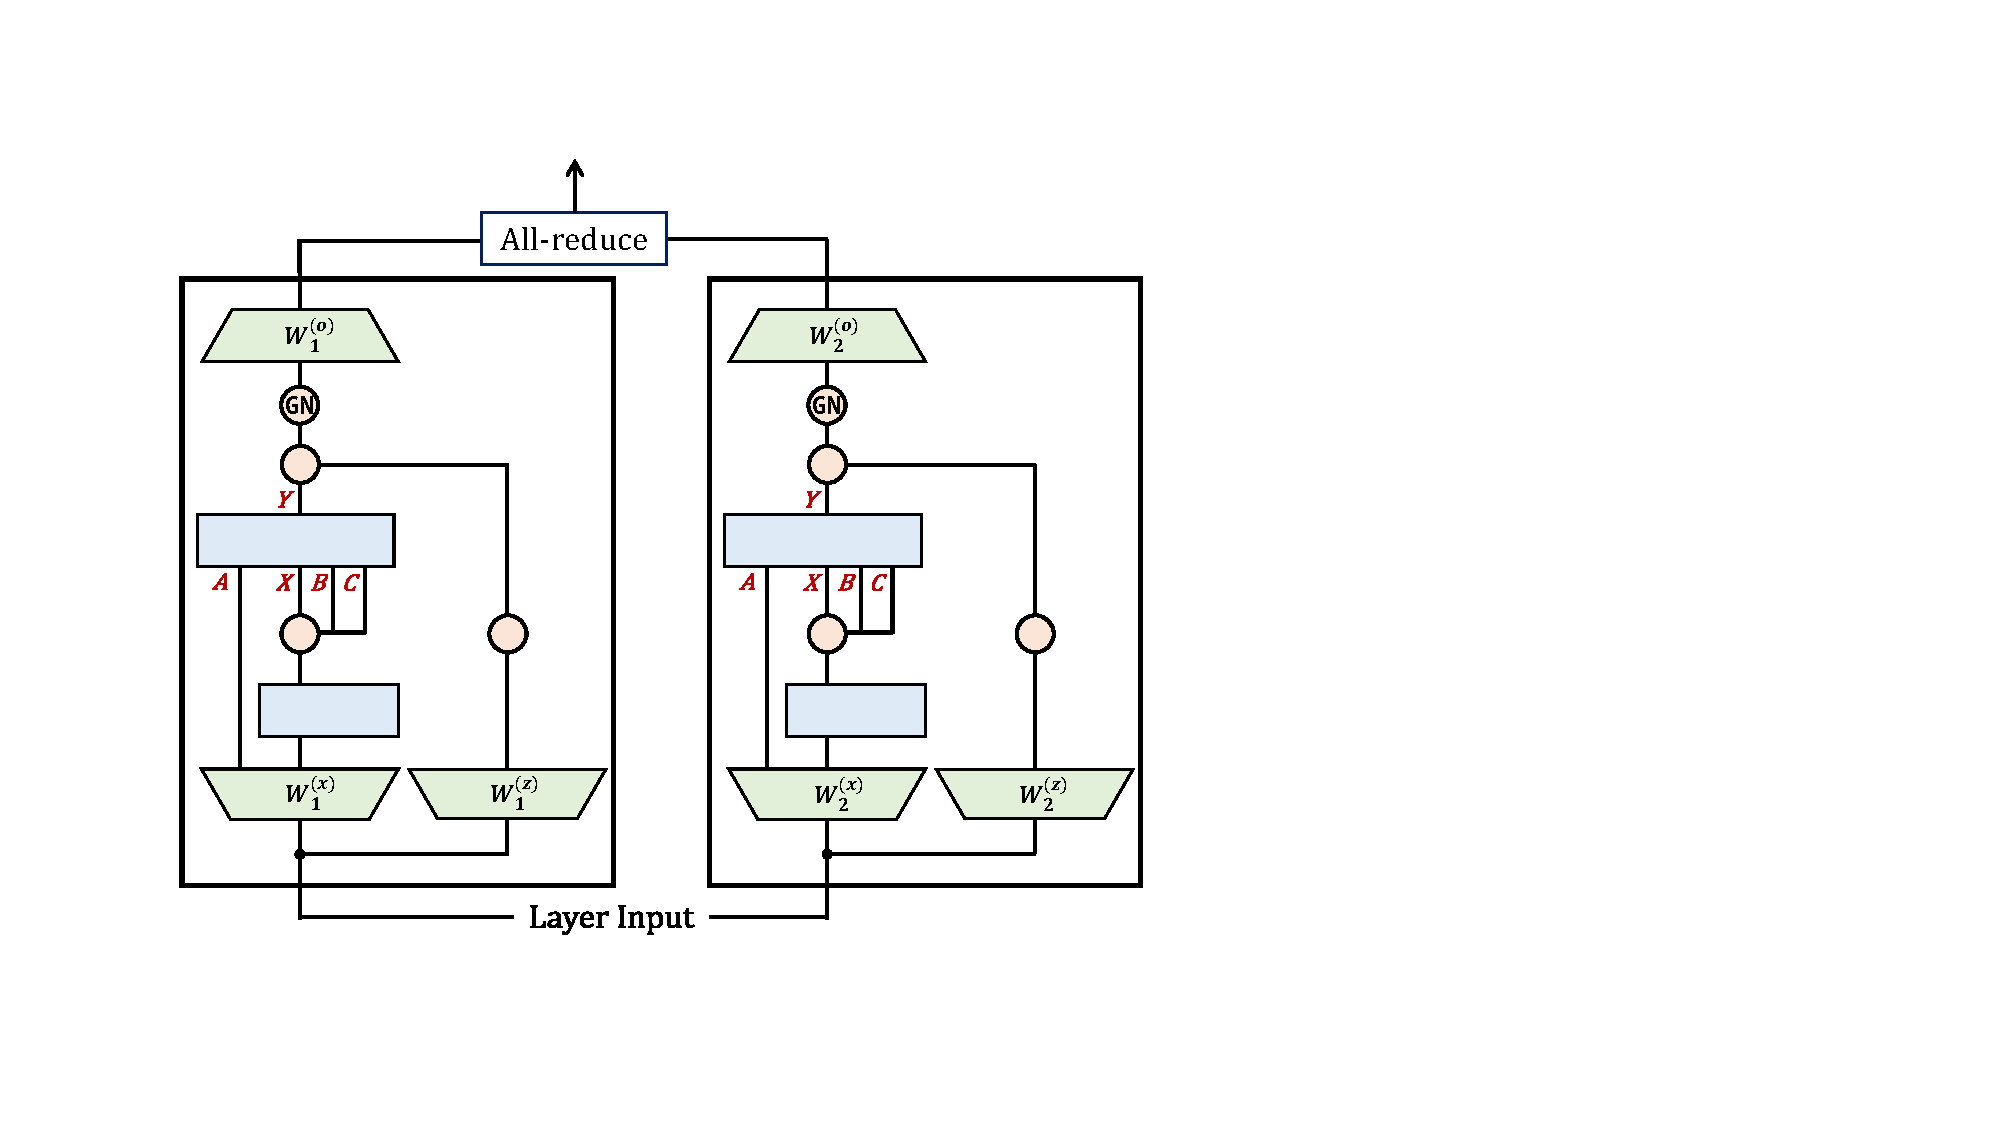
\includegraphics[width=\linewidth]{fig/mamba_tp.pdf}
\end{minipage}
\hfill
\begin{minipage}{.59\linewidth}%
  \centering
  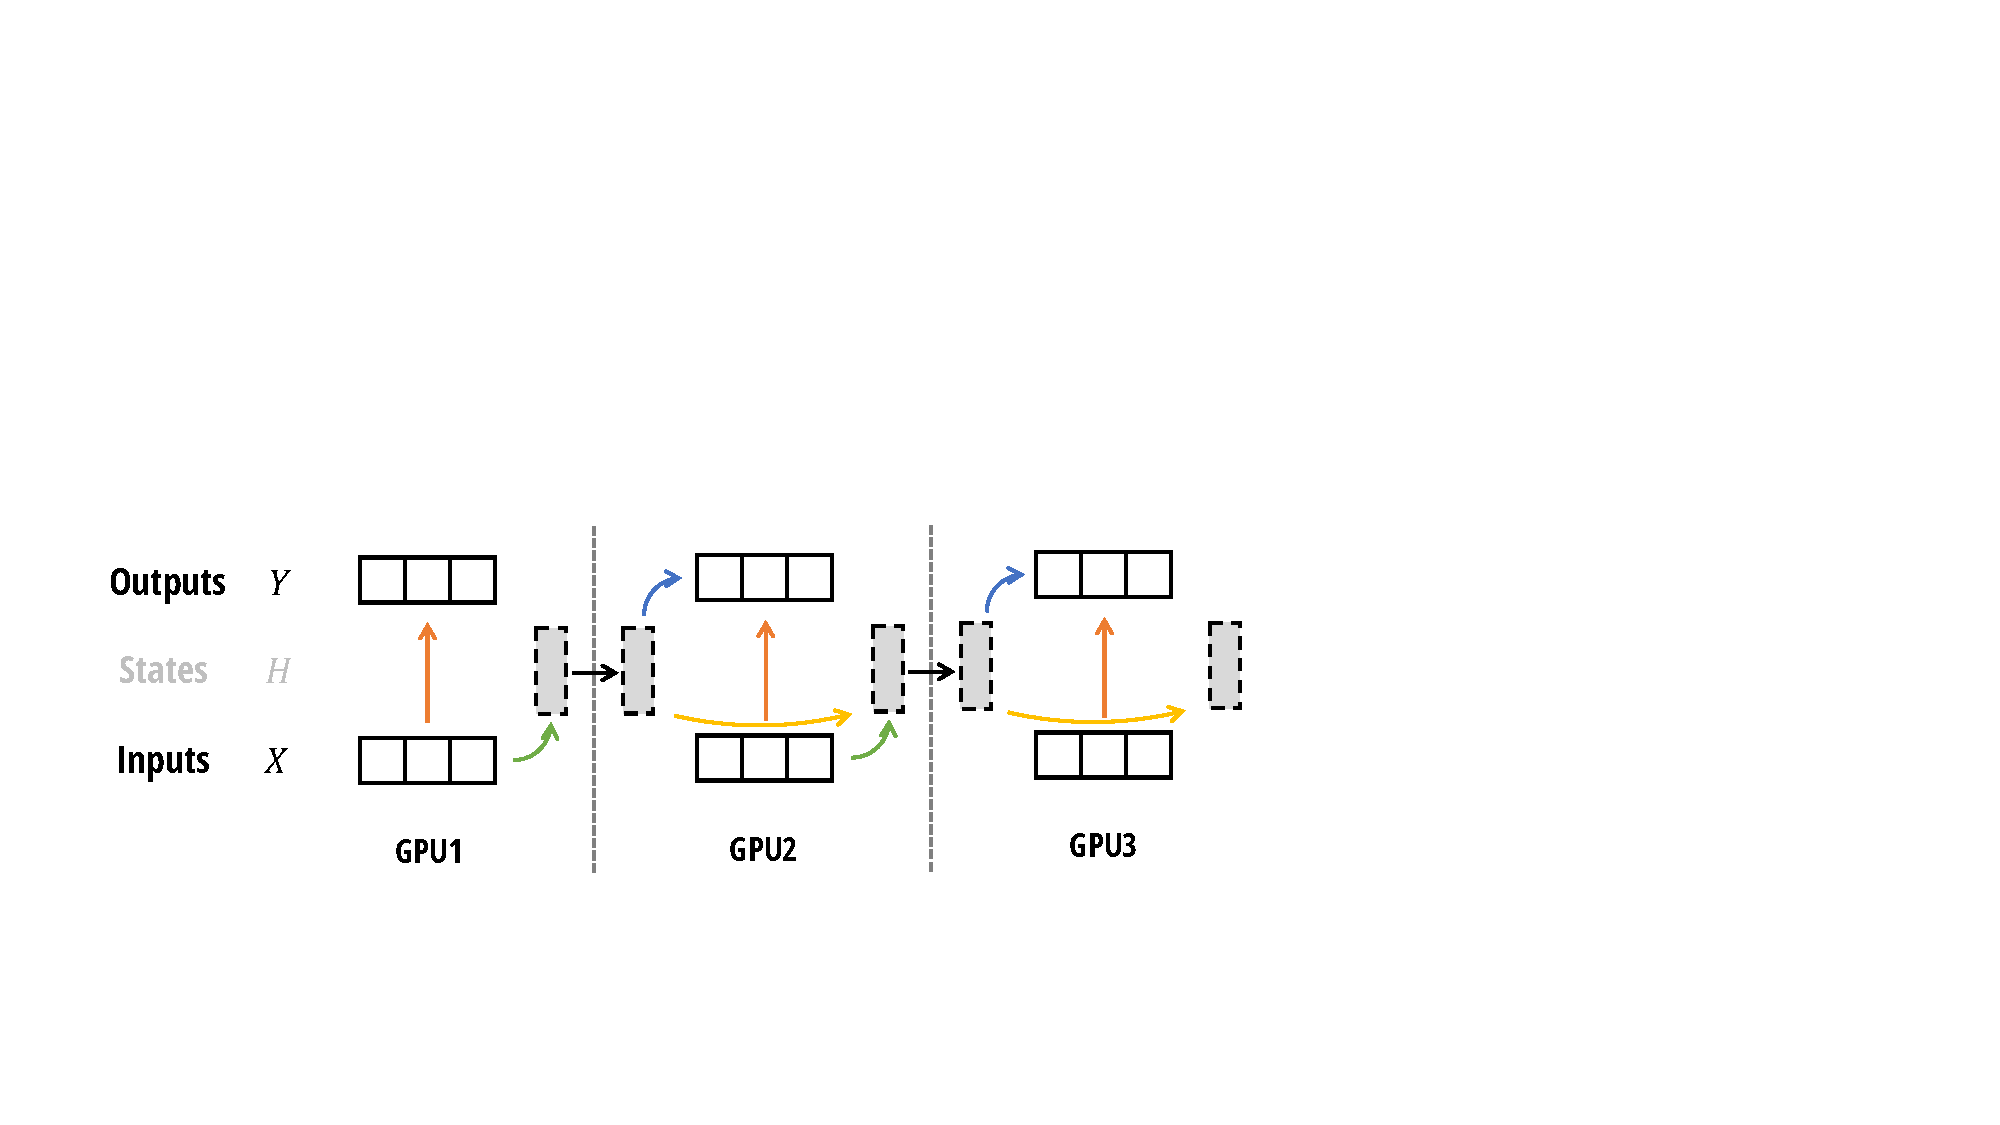
\includegraphics[width=\linewidth]{fig/mamba_cp.pdf}
\end{minipage}
\caption{
  (\textbf{Parallelism with the Mamba-2 Block}.)
  (\emph{Left}: \textbf{Tensor Parallelism})
  We split the input projection matrices $W^{(x)}, W^{(z)}$ and the output projection matrix $W^{(o)}$.
  Each SSM head $(A, B, C, X) \mapsto Y$ lives on a single device.
  Choosing GroupNorm for the final normalization layer avoids extra communication.
  We need one all-reduce per layer, just like the MLP or attention blocks in a Transformer.
  (\emph{Right}: \textbf{Sequence/Context Parallelism})
  Analogous to the SSD algorithm, with multiple devices, we can split along the sequence dimension. Each device computes the state of its sequence, then pass that state to the next GPU.
}
\label{fig:mamba2_parallelism}
\end{figure}

\subsection{Sequence Parallelism}
\label{subsec:sp}

For very long sequences, we might need to split the input and activation to different GPUs along the sequence length dimension.
There are two main techniques:
\begin{enumerate}
\item Sequence parallelism (SP) for the residual and normalization operations: first proposed by~\citet{korthikanti2023reducing}, this technique decomposes the all-reduce in TP as reduce-scatter and all-gather. Noticing that the residual and normalization operations are repeated on the same input for all GPUs in the same TP group, SP splits the activations along the sequence length dimension by performing: reduce-scatter, residual and normalization, then all-gather.

Since the Mamba-2 architecture uses the same residual and normalization structure, SP applies without modification.

\item Sequence parallelism for the token-mixing operations (attention or SSM), also known as ``context parallelism'' (CP).
Several techniques have been developed for attention layer (e.g., Ring attention~\citep{liu2023ring, liu2024world}), with sophisticated load-balancing technique~\citep{brandon2023striped}.
The difficulty with sequence parallelism in attention is that we can split queries and keys into block, but each query block needs to interact with key blocks, leading to communication bandwidth quadratic in the number of workers.

With SSMs, we can split the sequence in a simple manner: each worker takes an initial state, compute the SSM with respect to their inputs, return the final state, and pass that final state to the next worker.
The communication bandwidth is linear in the number of workers.
This decomposition is exactly the same as the block-decomposition in the SSD algorithm (\cref{fig:ssd-algorithm}) to split into blocks / chunks.
We illustrate this context parallelism in~\cref{fig:mamba2_parallelism} (\emph{Right}).

\end{enumerate}

\subsection{Variable Length}
\label{subsec:varlen}

While pretraining often uses the same sequence lengths for the batch, during finetuning or inference, the model might need to process different input sequences of different lengths.
One naive way to handle this case is to right-pad all sequences in the batch to the maximum length, but this can be inefficient if sequences are wildly different lengths.
For transformers, sophisticated techniques have been develop to avoid padding and do load-balancing between GPUs~\citep{zeng2022boosting, zhai2023bytetransformer}, or packing multiple sequences in the same batch and adjust the attention mask~\citep{ding2024fewer, pouransari2024dataset}.
With SSMs and Mamba in particular, we can handle variable sequence lengths by simply treating the whole batch as one long sequence, and avoid passing the states between individual sequences.
This is equivalent to simply setting $A_t = 0$ for tokens $t$ at the end of one sequence to prevent it from passing information to the token $t + 1$, which belongs to a different sequence.


\section{Experiments}
\label{sec:experiments}

We validate our approach empirically, showing that our Monarch matrix parametrization achieves a favorable efficiency--accuracy tradeoff compared to baselines on a wide range of domains (text, images, PDEs, MRI), in three settings (E2E training, S2D training, and D2S fine-tuning):
\begin{itemize}[leftmargin=*,nosep,nolistsep,noitemsep]
\item
In \cref{subsec:benchmark_tasks}, on image classification and language modeling benchmarks, such as ViT / MLP Mixer on ImageNet and GPT-2 on Wikitext-103, Monarch is 2$\times$ faster to train than dense models, while achieving the same accuracy / perplexity. In \cref{subsec:pde_mri}, in scientific and medical domains where special transforms (Fourier) are common, Monarch outperforms Fourier transform based methods on PDE solving, with up to 40\% lower error, and on MRI reconstruction attains up to 15\% higher pSNR and 3.8\% higher SSIM.
\item In \cref{subsec:pde_mri}, we show that on the large OpenWebText dataset, reverse sparsification (training with Monarch weight matrices for most of the time, then transitioning to dense weight matrices) speeds up the pretraining of GPT-2 models by 2$\times$ compared to the dense model, with no loss in upstream or downstream quality.
Moreover, reverse sparsification speeds up BERT pretraining by 23\% even compared to the implementation from Nvidia that set the MLPerf~\citep{mattson2020mlperf} 1.1 record.
\item In \cref{subsec:finetuning}, as a proof of concept, we demonstrate that our Monarch approximation algorithm can improve fine-tuning efficiency for pretrained models. We show that compressing BERT to a Monarch matrix model performs comparably to a finetuned dense model on GLUE, with 2$\times$ fewer parameters and 1.7$\times$ faster finetuning speed.
\end{itemize}

\subsection{End-to-End Training}
\label{subsec:e2e_training}
\subsubsection{Benchmark Tasks: Image Classification, Language Modeling}
\label{subsec:benchmark_tasks}

We show that replacing dense matrices with Monarch matrices in ViT, MLP-Mixer, and
GPT-2 can speed up training by up to 2$\times$ without sacrificing model quality in~\cref{table:pretrain,table:gpt_pretrain}.

\textbf{Setup.} We use the popular vision benchmark, ImageNet~\citep{deng2009imagenet}. We choose recent popular Vision Transformer~\citep{dosovitskiy2020image}, and MLP-Mixer~\citep{tolstikhin2021mlp} as representative base dense models.
For language modeling, we evaluate GPT-2~\citep{radford2019language} on WikiText-103~\citep{merity2016pointer}.

\begin{table}[h]
  \small
  \centering
  \vspace{-2mm}
  \caption{\label{table:pretrain}The performance of Monarch matrices and ViT / MLP-Mixer on ImageNet, including the number of parameters and FLOPs. We measure the Top-1 accuracy and the training time speedup compared to the corresponding dense model. %
  \vspace{2mm}
  }
  \iftoggle{arxiv}{}{
  \resizebox{\linewidth}{!}
  }
  {
  \setlength{\tabcolsep}{3pt}
  \vspace{3em}
  \begin{tabular}{@{}c||ccccccc@{}}
  \specialrule{.15em}{.05em}{.05em}
    Model&\multicolumn{1}{c}{ImageNet acc.}&\multicolumn{1}{c}{Speedup} &\multicolumn{1}{c}{Params} & \multicolumn{1}{c}{FLOPs} \\
    \specialrule{.15em}{.05em}{.05em}
    Mixer-S/16& 74.0& - & 18.5M & 3.8G \\
    Monarch-Mixer-S/16& 73.7& 1.7$\times$ & 7.0M & 1.5G \\
    Mixer-B/16& 77.7& - & 59.9M & 12.6G \\
    Monarch-Mixer-B/16& 77.8& 1.9$\times$ & 20.9M & 5.0G \\
    \specialrule{.15em}{.05em}{.05em}
    ViT-S/16& 79.4 & - & 48.8M & 9.9G \\
    Monarch-ViT-S/16& 79.1 & 1.9$\times$ & 19.6M & 3.9G \\
    ViT-B/16& 78.5 & - & 86.6M  & 17.6G \\
    Monarch-ViT-B/16& 78.9 & 2.0$\times$ & 33.0M & 5.9G \\
    \specialrule{.15em}{.05em}{.05em}
  \end{tabular}
  }
\end{table}

\begin{table}[h]
  \small
  \centering
  \vspace{-3mm}
  \caption{\label{table:gpt_pretrain} Performance of Monarch matrices and GPT-2-Small/Medium on WikiText-103, including the \# of parameters and FLOPs. Monarch achieves similar perplexity (ppl) but 2.0$\times$ faster.}
  \vspace{1mm}
  \iftoggle{arxiv}{}{
    \resizebox{0.95\linewidth}{!}
  }
  {
\setlength{\tabcolsep}{5pt}
\begin{tabular}{c||cccc}
\specialrule{.15em}{.05em}{.05em}
\multirow{1}{*}{{ Model} } & \multicolumn{1}{c}{\multirow{1}{*}{PPL}}
                              & \multicolumn{1}{c}{\multirow{1}{*}{Speedup}}
                              & \multicolumn{1}{c}{\multirow{1}{*}{Params}}
                              & \multicolumn{1}{c}{\multirow{1}{*}{FLOPs}}\\
\specialrule{.15em}{.05em}{.05em}
GPT-2-Small &  20.6 & - & 124M& 106G\\
Monarch-GPT-2-Small& 20.7  & 1.8$\times$ &72M & 51G\\
\specialrule{.15em}{.05em}{.05em}
GPT-2-Medium &  20.9 & - & 355M& 361G\\
Monarch-GPT-2-Medium& 20.3  & 2.0$\times$ &165M & 166G\\
\specialrule{.15em}{.05em}{.05em}
\end{tabular}
}
\vspace{-2mm}
\end{table}


\subsubsection{PDE solving and multi-coil MRI reconstruction}
\label{subsec:pde_mri}

Many scientific or medical imaging tasks rely on specialized transforms such as the
Fourier transform.
We show that replacing the fixed Fourier transform with the more expressive
Monarch matrices yields higher model quality (lower reconstruction error) with
comparable model speed.

\textbf{Solving PDEs with Monarch Neural Operators.}
We follow the experimental setting in FNO~\citep{li2020fourier} and apply a Monarch--based neural operator to the task of solving the Navier--Stokes PDE. Compared to baseline U-Nets~\citep{ronneberger2015u}, TF-Nets~\citep{wang2020towards}, ResNets~\citep{he2016deep} and FNOs~\cite{li2020fourier}, neural operators based on Monarch improve solution accuracy across spatial resolutions by up to $40\%$ (Table \ref{table:pde}).  





\paragraph{Non-periodic boundary conditions.} Traditional spectral methods based on Fourier transform work best with periodic boundary conditions and forcing terms. However, PDEs of practical interest often exhibit non--periodic or even unknown boundary conditions. Monarch operators are not constrained to the Fourier transform and can thus still learn the solution operator with excellent accuracy.

\begin{table}[h!] 
\scriptsize
\vspace{-4mm}
\caption{\label{table:pde}Benchmarks on Navier-Stokes (fixing resolution 64 × 64 for both training and testing).
Decreasing the viscosity coefficient $\nu$ makes the dynamics more chaotic.
}
\vspace{1mm}
\centering
\iftoggle{arxiv}{}{
  \resizebox{0.9\linewidth}{!}
}
{
\renewcommand{\arraystretch}{1}
\begin{tabular}{ c||ccc }
\specialrule{.15em}{.05em}{.05em}
Model & $v = 10^{-3}$  &  $v = 10^{-4}$ & $v = 10^{-5}$\\
\specialrule{.15em}{.05em}{.05em}
U-Net & 0.025  & 0.205  &   0.198\\
TF-Net  & 0.023  & 0.225 &  0.227 \\
ResNet & 0.070 &  0.287 &  0.275 \\
FNO & 0.017  & 0.178 & 0.155\\
Monarch-NO & \textbf{0.010} & \textbf{0.145} & \textbf{0.136} \\
\specialrule{.15em}{.05em}{.05em}
\end{tabular}
}
\textbf{\vspace{-3mm}}
\end{table}

\textbf{Accelerated MRI Reconstruction.} We characterize the utility of Monarch-based FFT operations for accelerated MRI reconstruction, a task which requires methods with both structured Fourier operators and dealiasing properties to recover high quality images. On the clinically-acquired 3D MRI SKM-TEA dataset \citep{desai2021skm}, Monarch-SENSE (mSENSE) enhances image quality by over 1.5dB pSNR and 2.5\% SSIM compared to zero-filled SENSE and up to 4.4dB and 3.8\% SSIM compared to U-Net baselines in data-limited settings. Setup details are available in~\cref{sec:experiment_details_mri}.

\paragraph{Expressive FFT.} By definition, standard IFFT in zero-filled SENSE cannot dealias the signal, resulting in artifacts in the reconstructed image. mSENSE replaces the inverse FFT (IFFT) operation in standard SENSE with learnable Monarch matrices. Thus, mSENSE preserves the structure of the Fourier transform while learning to reweight frequencies to suppress aliasing artifacts. Across multiple accelerations, mSENSE achieved up to +1.5dB and 2.5\% improvement in peak signal-to-noise ratio (pSNR) and structural similarity (SSIM), respectively (Table~\ref{table:mri}).

\paragraph{Data Efficiency.} While CNNs have shown promise for MRI reconstruction tasks, training these networks requires extensive amounts of labeled data to avoid overfitting. However, large data corpora are difficult to acquire in practice. mSENSE can be trained efficiently with limited supervised examples. In few shot settings, mSENSE can outperform U-Net by +4.4dB ($\approx$15\%) and 3.8\% SSIM (Table~\ref{table:mri-data-limited}). 







\begin{table}[h!] 
\scriptsize
\vspace{-3mm}
\caption{\label{table:mri}Mean $\pm$ standard error of the mean of conventional and Monarch-SENSE (mSENSE) on dual-echo (E1,E2) MRI reconstruction at multiple acceleration factors (Acc.).
}
\vspace{1mm}
\centering
\iftoggle{arxiv}{}{
  \resizebox{\linewidth}{!}
}
{
\renewcommand{\arraystretch}{1.2}
\begin{tabular}{c||ccccc}
\specialrule{.15em}{.05em}{.05em}
  & & \multicolumn{2}{c}{pSNR (dB) ($\uparrow$)} & \multicolumn{2}{c}{SSIM ($\uparrow$)} \\
  Acc. & Model &             E1 &             E2 &                E1 &                E2 \\
\specialrule{.15em}{.05em}{.05em}
\multirow{2}{*}{2} & SENSE &  32.8$\pm$0.2 &  35.4$\pm$0.2 &  0.871$\pm$0.003 &  0.865$\pm$0.003 \\
  & mSENSE &  \textbf{34.3$\pm$0.2} &  \textbf{36.6$\pm$0.2} &  \textbf{0.886$\pm$0.002} &  \textbf{0.882$\pm$0.003} \\
\specialrule{.15em}{.05em}{.05em}
\multirow{2}{*}{3} & SENSE &  30.9$\pm$0.2 &  33.5$\pm$0.2 &  0.819$\pm$0.004 &  0.795$\pm$0.004 \\
  & mSENSE &  \textbf{32.3$\pm$0.2} &  \textbf{34.6$\pm$0.2} &  \textbf{0.843$\pm$0.003} &  \textbf{0.820$\pm$0.004} \\
\specialrule{.15em}{.05em}{.05em}
\multirow{2}{*}{4} & SENSE &  30.1$\pm$0.2 &  32.8$\pm$0.2 &  0.789$\pm$0.004 &  0.753$\pm$0.005 \\
  & mSENSE &  \textbf{31.2$\pm$0.2} &  \textbf{33.5$\pm$0.2} &  \textbf{0.812$\pm$0.003} &  \textbf{0.767$\pm$0.005} \\
\specialrule{.15em}{.05em}{.05em}
\end{tabular}
}
\end{table}

\begin{table}[h!] 
\scriptsize
\vspace{-5mm}
\caption{\label{table:mri-data-limited}Impact of number of training examples ($N$) on dual-echo MRI reconstruction at 2x acceleration.
}
\vspace{1mm}
\centering
\iftoggle{arxiv}{}{
  \resizebox{\linewidth}{!}
}
{
\renewcommand{\arraystretch}{1.2}
\begin{tabular}{c||ccccc}
\specialrule{.15em}{.05em}{.05em}
  &  & \multicolumn{2}{c}{pSNR (dB) ($\uparrow$)} & \multicolumn{2}{c}{SSIM ($\uparrow$)} \\
  $N$ & Model &            E1 &            E2 &               E1 &               E2 \\
\specialrule{.15em}{.05em}{.05em}
N/A & SENSE &  32.8$\pm$0.2 &  35.4$\pm$0.2 &  0.871$\pm$0.003 &  0.865$\pm$0.003 \\
\specialrule{.15em}{.05em}{.05em}
\multirow{2}{*}{1} & U-Net &  29.4$\pm$0.2 &  34.4$\pm$0.3 &  0.848$\pm$0.004 &  0.857$\pm$0.004 \\
  & mSENSE &  \textbf{33.8$\pm$0.2} &  \textbf{36.0$\pm$0.2} &  \textbf{0.886$\pm$0.003} &  \textbf{0.867$\pm$0.003} \\
\specialrule{.15em}{.05em}{.05em}
\multirow{2}{*}{2} & U-Net &  29.9$\pm$0.3 &  35.1$\pm$0.3 &  0.858$\pm$0.003 &  0.871$\pm$0.003 \\
  & mSENSE &  \textbf{34.0$\pm$0.2} &  \textbf{36.4$\pm$0.2} &  \textbf{0.883$\pm$0.002} &  \textbf{0.877$\pm$0.003} \\
\specialrule{.15em}{.05em}{.05em}
\multirow{2}{*}{3} & U-Net &  31.0$\pm$0.3 &  35.2$\pm$0.3 &  0.866$\pm$0.003 &  0.867$\pm$0.004 \\
  & mSENSE &  \textbf{33.9$\pm$0.2} & \textbf{ 36.5$\pm$0.2} &  \textbf{0.882$\pm$0.002} & \textbf{0.878$\pm$0.003} \\
\specialrule{.15em}{.05em}{.05em}
\multirow{2}{*}{5} & U-Net &  31.4$\pm$0.3 &  35.6$\pm$0.2 &  0.877$\pm$0.002 &  0.870$\pm$0.003 \\
  & mSENSE &  \textbf{33.9$\pm$0.2} &  \textbf{36.5$\pm$0.2} &  \textbf{0.881$\pm$0.002} &  \textbf{0.877$\pm$0.003} \\
\specialrule{.15em}{.05em}{.05em}
\end{tabular}
}
\end{table}




\subsection{Sparse-to-Dense Training (reverse sparsification)}
\label{subsec:s2d_training}
\paragraph{GPT-2 pretraining.}
On the large OpenWebtext dataset~\citep{Gokaslan2019OpenWeb}, we train a GPT-2 model with Monarch weight
matrices for 90\% of the training iterations, then relax the constraint on the
weight matrices and train them as dense matrices for the remaining 10\% of the
iterations.
We call this technique ``reverse sparsification.''
Previous sparse training techniques often don't speed up training, whereas our
hardware-efficient Monarch matrices do.
Therefore we can use them as an intermediate step to pretrain a large language
model (GPT-2) in 2$\times$ less time. We also evaluate its downstream quality on zero-shot generation from~\citep{eval-harness} and classification tasks from~\citep{zhao2021calibrate}, achieving comparable performance to the dense counterparts (\cref{table:gpt_finetune}). 

\begin{table}[h]
  \small
  \centering
  \vspace{-3mm}
  \caption{\label{table:gpt_finetune}The performance (accuracy) of GPT-2-medium trained with Monarch reverse sparsification and with conventional dense training on text classification benchmarks.}
  \setlength{\tabcolsep}{5pt}
  \vspace{1em}
  \iftoggle{arxiv}{}{
    \resizebox{\linewidth}{!}
  }
  {
  \begin{tabular}{@{}c||ccc@{}}
    \specialrule{.15em}{.05em}{.05em}
    Model&\multicolumn{1}{c}{OpenWebText (ppl)}&\multicolumn{1}{c}{Speedup}& \multicolumn{1}{c}{Classification (avg acc)} \\
    \specialrule{.15em}{.05em}{.05em}
    GPT-2m& 18.0 & - & 38.9 \\
    Monarch-GPT-2m& 18.0 & 2$\times$ & 38.8 \\
    \specialrule{.15em}{.05em}{.05em}
  \end{tabular}
  }
  \vspace{-3mm}
\end{table}


In \cref{fig:reverse_sparsification_bar}, we show the training time of the dense GPT-2 model, along with
the Monarch GPT-2 model.
After training the Monarch model for 90\% of the time, in the
last 10\% of the training steps, by transitioning to dense weight matrices, the model is able to reach the same 
performance of another model that was trained with dense weight matrices from
scratch.
By training with Monarch matrices for 90\% of the time, we reduce the total training time by 2$\times$.

\paragraph{BERT pretraining.}
On the Wikipedia + BookCorpus datasets~\citep{zhu2015aligning}, we train a BERT-large model with Monarch weight matrices for 70\% of the time and transition to dense weight matrices for the remaining 30\% of the time, which yields the same pretraining loss as conventional dense training.
In \cref{table:bert_speed}, we compare the total training time to several baseline implementations: the widely-used implementation from HuggingFace~\citep{wolf-etal-2020-transformers}, the more optimized implementation from Megatron~\citep{shoeybi2019megatron}, and the most optimized implementation we know of from Nvidia that was used to set MLPerf 1.1 training speed record. Our method is 3.5x faster than HuggingFace and 23\% faster than Nvidia's MLPerf 1.1 implementation\footnote{Our result is not an official MLPerf submission. We train BERT for both phase 1 (sequence length 128) and phase 2 (sequence length 512) according to the standard BERT training recipe\cite{devlin2018bert}, while MLPerf only measures training time for phase 2.}.
Experiment details are in~\cref{subsec:bert_details}.

\begin{table}[h]
  \small
  \centering
  \caption{\label{table:bert_speed}The total training time of BERT-large trained with Monarch reverse sparsification and with conventional dense training on 8 A100-40GB GPUs (DGX A100). Training consists of two phases, phase 1 with sequence length 128 and phase 2 with sequence length 512. Monarch training is 3.5x faster than HuggingFace and 23\% faster than Nvidia's MLPerf 1.1 implementation.}
  \vspace{1em}
  \iftoggle{arxiv}{}{
    \resizebox{\linewidth}{!}
  }
  {
    \begin{tabular}{@{}c||c@{}}
      Implementation & Training time (h)  \\ \hline
      HuggingFace &  84.5 \\
      MegaTron & 52.5 \\
      Nvidia MLPerf 1.1 & 30.2 \\
      Nvidia MLPerf 1.1 + DeepSpeed & 29.3 \\
      Monarch (ours) & \textbf{23.8} \\
    \end{tabular}
  }
  \vspace{-3mm}
\end{table}

\subsection{Dense-to-Sparse Fine-tuning}
\label{subsec:finetuning}

\begin{figure}[t]
  \centering
  \vspace{-3mm}
  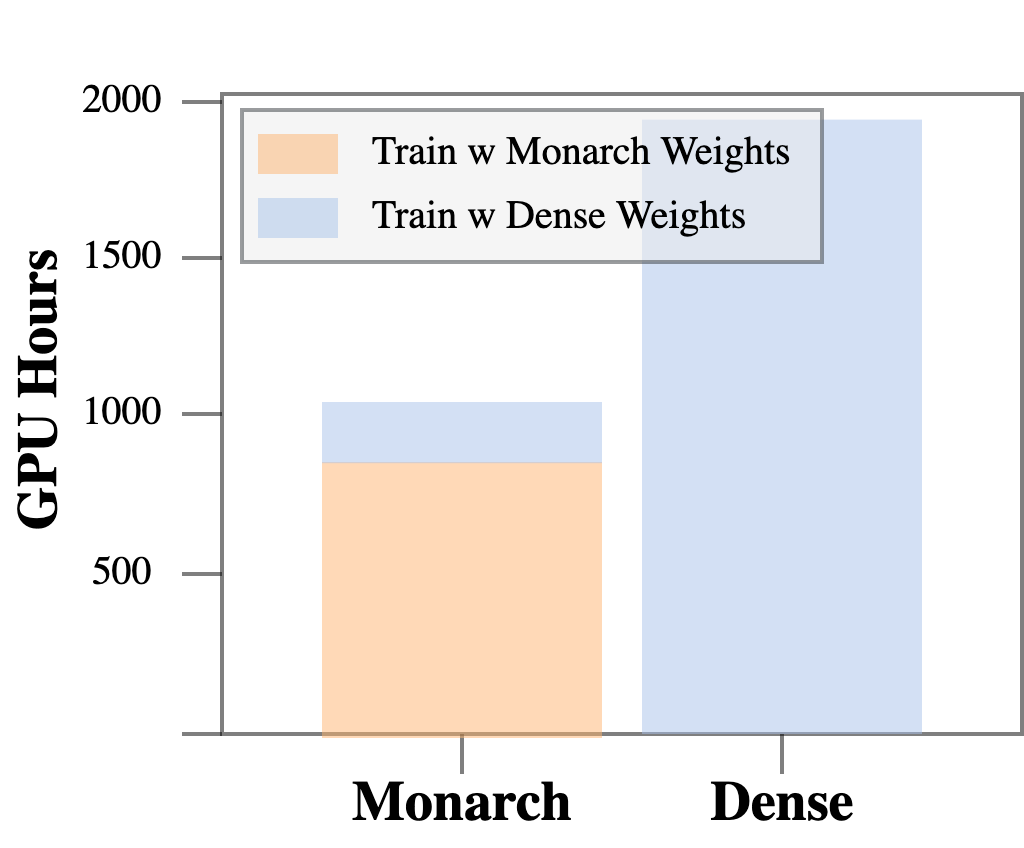
\includegraphics[width=.3\textwidth]{figures/rv_bar_temp.png}
  \vspace{-3mm}
  \caption{\label{fig:reverse_sparsification_bar}Time required (in A100 GPU hours) to reach the same perplexity (18.0)
    for GPT-2-small on OpenWebText.
    With ``reverse sparsification'', Monarch can speed up
    GPT-2 training by 2$\times$.\vspace{-1em}}
\end{figure}

We show that our Monarch approximation algorithm allows us to efficiently use
pretrained models, such as speeding up BERT finetuning on GLUE.

\paragraph{BERT finetuning.}
We take the BERT pretrained weights, approximate them with Monarch matrices,
and finetune the resulting model on the 9 GLUE tasks.
The results in \cref{table:bert_glue} shows that we obtain a Monarch finetuned
model with similar quality to the dense BERT model, but with 1.7$\times$ faster
finetuning speed.
This serves as a proof of concept, and we expect further speedup if additional model compression techniques are applied (e.g., quantization, kernel fusion).




\begin{table}[h]
  \small
  \centering
  \vspace{-5mm}
  \caption{\label{table:bert_glue}The performance of Monarch matrices in
    finetuning BERT on GLUE.}
  \setlength{\tabcolsep}{5pt}
  \vspace{1em}
  \iftoggle{arxiv}{}{
    \resizebox{\linewidth}{!}
  }
  {
  \begin{tabular}{@{}c||ccccccc@{}}
  \specialrule{.15em}{.05em}{.05em}
    Model&\multicolumn{1}{c}{GLUE (avg)}&\multicolumn{1}{c}{Speedup} &\multicolumn{1}{c}{Params} & \multicolumn{1}{c}{FLOPs} \\
    \specialrule{.15em}{.05em}{.05em}
    BERT-base & 78.6& - & 109M & 11.2G \\
    Monarch-BERT-base& 78.3& 1.5$\times$ & 55M & 6.2G  \\
    BERT-large & 80.4 & - & 335M & 39.5G \\
    Monarch-BERT-large & 79.6 & 1.7$\times$ & 144M & 14.6G  \\
    \specialrule{.15em}{.05em}{.05em}
  \end{tabular}
  }
  \vspace{-3mm}
\end{table}



%!TEX root = ../main.tex

\section{Related Work}
\label{sec:related}

\textbf{State space models} have shown promise in modeling sequential data, including time series data~\citep{gu2022efficiently}, audio~\citep{goel2022s}, and visual data~\citep{nguyen2022s4nd}.
Our model builds off work on simplifying and parameterizing diagonal versions of S4~\citep{gu2022parameterization,gupta2022diagonal, gu2022train}.
Gated state spaces~\citep{mehta2022long} also aim to adapt SSMs to language modeling, but our results suggest that the GSS model does not perform as well as \hthree (or even as well as earlier SSMs like S4D).
The idea to combine SSMs with attention in hybrid models is not new; Mehta et al.~\citep{mehta2022long} also showed that interleaving attention with their GSS layer can improve performance, which we also validate on our OpenWebText experiments.
These positive results suggest that attention and SSMs are complementary, and that hybrid models may be a promising direction for future work.

\textbf{Large language foundation models}~\citep{bommasani2021opportunities} have demonstrated the power of scaling attention-based networks to billions of parameters and training them on trillions of tokens~\citep{hoffmann2022training}.
Understanding the mechanistic basis~\citep{elhage2021mathematical} behind these models may yield insights into better design choices for future models.
These and similar explorations have informed the design of \hthree and our selection of synthetic languages.
A number of recent works have also explored how to address the shortcomings of attention by approximating the attention computation~\citep{wang2020linformer,katharopoulos2020transformers, choromanski2020rethinking,tay2020long, kitaev2020reformer, daras2020smyrf}.
We believe these efforts are complementary to SSMs, and we are excited to see how they can be combined in future work.

\textbf{Linear attention}~\citep{katharopoulos2020transformers} and classical sequence models like RNNs serve as inspiration for \hthree.
Appendix~\ref{app:linear_attention} draws a direct connection between linear attention and LTI systems.
Luo et al.~\citep{luo2021stable} also propose a variant of linear attention that can achieve $O(n \log n)$ scaling in sequence length.
Appendix~\ref{sec:app_additional_experiments} evaluates linear attention on language modeling, and finds that it underperforms exact attention, whereas \hthree outperforms attention.
The multiplicative interactions in \hthree are reminiscent of gating mechanisms in LSTMs~\citep{hochreiter1996lstm} and GRUs~\citep{cho2014properties}, which suggests that architectural lessons from these sequence models may be useful for adapting SSMs to language modeling.
A number of algorithms for scaling attention to longer sequences have also been proposed, such as Transformer-XL~\citep{dai2019transformer}, Reformer~\citep{kitaev2020reformer}, Performer~\citep{choromanski2020rethinking}, and Perceiver AR~\citep{hawthorne2022general}.
Some of these approaches underperform exact attention on language modeling, and may be slower in wall-clock speed~\citep{dao2022flashattention}.
A thorough comparison of these alternatives to exact attention and how well they scale in model size and amount of training data is fruitful future work.

\textbf{FFT} algorithms are used in a wide variety of applications, including signal processing~\citep{oppenheim1978applications}, control theory~\citep{brogan1974modern}, and more.
Various algorithms for computing the FFT have existed for decades~\citep{oppenheim2001discrete}.
We hope our work on appealing to these classic algorithms to accelerate new applications such as learned SSMs will inspire future algorithmic exploration, even if hardware is not designed for them~\citep{hooker2021hardware}.

%%% Local Variables:
%%% mode: latex
%%% TeX-master: "../main"
%%% End:


Hyperbolic embeddings embed hierarchical information with high
fidelity and few dimensions. We explored the limits of this approach
by describing scalable, high quality algorithms. We hope the
techniques here encourage more follow-on work on the exciting
techniques of \citet{fb, ucl}. As future work, we hope to explore how
hyperbolic embeddings can be most effectively incorporated into downstream
tasks and applications.


\subsubsection*{Acknowledgments}
We thank Angela Wu for the suggestion on how to efficiently compute
the gradient of $\Delta$ in a numerically stable manner.
We thank Sukjun Hwang and Aakash Lahoti for assistance with the MQAR experiments.



\printbibliography

\newpage

\appendix

\onecolumn

  \section{Glossary}
\label{sec:glossary}

\begin{table}[!h]
  \caption{
    Glossary of notation and terminology; mnemonics bolded.
    (\emph{Top}) Frequently used tensor dimensions.
    (\emph{Bottom}) Matrices and tensors used in state space models or structured masked attention.
  }
  \centering
  \begin{tabular}{@{}lll@{}}
    \toprule
    Notation       & Description                                                                & Definition \\
    \midrule
    $\mathtt{T}$   & \textbf{Time} axis or \textbf{target} sequence axis                        & \cref{def:sequence-transformation} \\
    $\mathtt{S}$   & \textbf{Source} sequence axis (in attention)                               & \cref{eq:kernel-attention} \\
    $\mathtt{D}$   & Model \textbf{dimension} or $\mathtt{d\_model}$                            & \cref{def:head-pattern} \\
    $\mathtt{N}$   & State/feature dimension or $\mathtt{d\_state}$                             & \cref{eq:s6,eq:kernel-attention} \\
    $\mathtt{P}$   & Head dimension or $\mathtt{d\_head}$                                       & \cref{def:sequence-transformation} \\
    $\mathtt{H}$   & Number of \textbf{heads} or $\mathtt{n\_head}$                             & \cref{def:head-pattern} \\
    \midrule
    $M$            & Sequence transformation \textbf{matrix}                                    & \cref{def:matrix-transformation} \\
    $A$            & Discrete SSM recurrent (state) matrix                                      & \cref{eq:s6} \\
    $B$            & State space model input projection (expansion) matrix                      & \cref{eq:s6} \\
    $C$            & State space model output projection (contraction) matrix                   & \cref{eq:s6} \\
    $X$            & Input matrix (shape $\mathtt{(T, P)}$)                                     & \cref{eq:s6,eq:kernel-attention} \\
    $Y$            & Output matrix (shape $\mathtt{(T, P)}$)                                    & \cref{eq:s6,eq:kernel-attention} \\
    $Q$            & Attention \textbf{query} matrix                                            & \cref{eq:kernel-attention} \\
    $K$            & Attention \textbf{key} matrix                                              & \cref{eq:kernel-attention} \\
    $V$            & Attention \textbf{value} matrix                                            & \cref{eq:kernel-attention} \\
    $G$            & Attention \textbf{Gram} matrix                                             & $QK^{\top}$ (or $CB^{\top}$) \\
    $L$            & (Structured) mask matrix (\textbf{lower}-triangular in the causal setting) & \cref{def:sma} \\
    \bottomrule
  \end{tabular}
  \label{tab:glossary}
\end{table}

\section{Efficient Algorithms for the Scalar SSM Scan (1-SS Multiplication)}
\label{sec:scan}

In this section we flesh out various algorithms for computing the scalar SSM scan, through the lens of structured matrix decompositions.
The scalar SSM scan is defined as computing the recurrent part of the discrete SSM \eqref{eq:1ss-recurrence},
in the case when $N=1$ (i.e.\ $A$ is a scalar).
This is commonly used to compute SSMs recurrently;
in particular, the case of structured SSMs where $A$ is diagonally structured reduces down to this operation,
such as in the S5~\citep{smith2023s5} and S6~\citep{gu2023mamba} models.

The goal of this section is to support a central theme of this paper that \emph{efficient algorithms for sequence models can be viewed as structured matrix multiplication algorithms}.
The various matrix decomposition ideas we show here are related to ideas used to derive fast SSM algorithms (\cref{sec:efficient}),
as well as directly used as a subroutine.


\subsection{Problem Definition}
Let $a : \mathtt{(D,)}$ and $b : \mathtt{(D,)}$ be sequences of scalars.
The \textbf{scalar SSM scan} is defined as
\begin{equation}%
  \label{eq:ssm-scan}
  h_t = a_t h_{t-1} + b_t
  .
\end{equation}
Here $h_{-1}$ can be an arbitrary value representing the previous \emph{hidden state} to the SSM recurrence;
unless otherwise specified, we assume $h_{-1} = 0$.

We also call equation \eqref{eq:ssm-scan} the \textbf{\texttt{cumprodsum}} (cumulative product sum).
Note that the \texttt{cumprodsum} reduces to the \texttt{cumprod} (cumulative product) when $b = 0$ is the additive identity and it reduces to the \texttt{cumsum} (cumulative sum) when $a=1$ is the multiplicative identity.

Finally, note that in vectorized form we can write
\begin{align*}%
  h &= M b \\
  M &=
  \begin{bmatrix}
    1 & \\
    a_1 & 1 & \\
    a_2a_1 & a_2 & 1 \\
    \vdots & \vdots & \ddots & \ddots \\
    a_{T-1}\dots a_1 & a_{T-1}\dots a_2 & \dots & a_{T-1} & 1 \\
  \end{bmatrix}
\end{align*}
In other words, this is simply the matrix-vector product by a 1-SS matrix $M$.

Therefore we have three ways of viewing this fundamental primitive operation that are all equivalent:
\begin{itemize}
  \item A (scalar) SSM scan.
  \item A \texttt{cumprodsum}.
  \item A 1-SS matrix-vector multiplication .
\end{itemize}

\subsection{Classical Algorithms}

We first describe the two classical ways of computing the SSM scan \eqref{eq:ssm-scan},
previously used by prior work.

\subsubsection{Sequential Recurrence}
\label{sec:scan:recurrence}

The recurrent mode simply computes \eqref{eq:ssm-scan} one timestep $t$ at a time.
From the perspective of 1-SS multiplication, this was also described in \cref{sec:ssm:algorithms:linear}.

\subsubsection{Parallel Associative Scan}
\label{sec:scan:classical:parallel}

Second, an important observation is that this recurrence can be turned into an associative scan~\citep{martin2018parallelizing,smith2023s5}.
This fact is not completely obvious.
For example, S5 defined the correct associative scan operator and then showed associativity of the operator through rote calculation.

A slightly cleaner way to see that this is computable with an associative scan is to turn the multi-term recurrence into a single-term recurrence on a hidden state of size $2$ instead of $1$:
\begin{align*}%
  h_t &= a_t h_{t-1} + b_t
  \\
  \begin{bmatrix} h_t \\ 1 \end{bmatrix}
      &=
  \begin{bmatrix}
    a_t & b_t \\ 0 & 1
  \end{bmatrix}
  \begin{bmatrix} h_{t-1} \\ 1 \end{bmatrix}
  .
\end{align*}
Then computing all the $h_t$ is the same as taking the cumulative products of these $2 \times 2$ matrices.
Since matrix multiplication is associative,
this can be computed with an associative scan.
The associative binary operator is simply matrix multiplication on these particular matrices:
\begin{align*}%
  \begin{bmatrix}
    a_t & b_t \\ 0 & 1
  \end{bmatrix}
  \begin{bmatrix}
    a_s & b_s \\ 0 & 1
  \end{bmatrix}
  =
  \begin{bmatrix}
    a_ta_s & a_tb_s + b_t \\ 0 & 1
  \end{bmatrix}
  .
\end{align*}
Equating the top row yields the same associative scan operator as defined by S5:
\begin{equation}%
  \label{eq:scan:associative-operator}
  (a_t, b_t) \otimes (a_s, b_s) = (a_ta_s, a_tb_s + b_t)
  .
\end{equation}

The reason why associative scans are important is that they can be parallelized using a divide-and-conquer algorithm~\citep{blelloch1990prefix}.
We omit the details of this algorithm, and instead show that the entire associative SSM scan algorithm can be derived from scratch through matrix decompositions (\cref{sec:scan:associative}).

\subsection{Efficient Algorithms via Structured Matrix Decompositions}

We discuss several algorithms for computing the SSM scan, all through the lens of finding structured matrix decompositions of the 1-SS matrix $M$.
These algorithms or computation modes include
\begin{itemize}
  \item A \emph{dilated} mode where information is propagated $1, 2, 4, 8, \dots$ steps at a time.
  \item A \emph{state-passing} mode where information is propagated forward in chunks.
  \item A \emph{fully recurrent} mode that increments one step at a time, which is a special case of the state-passing mode.
  \item A \emph{block decomposition} parallel mode where $M$ is divided into hierarchical blocks.
  \item A \emph{scan} mode where $M$ is divide into equal size blocks and reduced recursively.
\end{itemize}

\subsubsection{Dilated Mode}

This mode factors the 1-SS matrix in a particular way involving increasing ``strides''.
This is best illustrated through a concrete example:
\footnotesize
\begin{align*}%
  M &=
  \begingroup
  \setlength\arraycolsep{2pt}
  \begin{bmatrix}
    a_{0:0} & \\
    a_{1:0} & a_{1:1} & \\
    a_{2:0} & a_{2:1} & a_{2:2} \\
    a_{3:0} & a_{3:1} & a_{3:2} & a_{3:3} \\
    a_{4:0} & a_{4:1} & a_{4:2} & a_{4:3} & a_{4:4} \\
    a_{5:0} & a_{5:1} & a_{5:2} & a_{5:3} & a_{5:4} & a_{5:5} \\
    a_{6:0} & a_{6:1} & a_{6:2} & a_{6:3} & a_{6:4} & a_{6:5} & a_{6:6} \\
    a_{7:0} & a_{7:1} & a_{7:2} & a_{7:3} & a_{7:4} & a_{7:5} & a_{7:6} & a_{7:7} \\
  \end{bmatrix}
  \endgroup
  \\&=
  \begingroup
  \setlength\arraycolsep{2pt}
  \begin{bmatrix}
    a_{0:0} & \\
            & a_{1:1} & \\
            &         & a_{2:2} \\
            &         &         & a_{3:3} \\
    a_{4:0} &         &         &         & a_{4:4} \\
            & a_{5:1} &         &         & & a_{5:5} \\
            &         & a_{6:2} &         & & & a_{6:6} \\
            &         &         & a_{7:3} & & & & a_{7:7} \\
  \end{bmatrix}
  \begin{bmatrix}
    a_{0:0} & \\
            & a_{1:1} & \\
    a_{2:0} &         & a_{2:2} \\
            & a_{3:1} &         & a_{3:3} \\
            &         & a_{4:2} &         & a_{4:4} \\
            &         &         & a_{5:3} &         & a_{5:5} \\
            &         &         &         & a_{6:4} &         & a_{6:6} \\
            &         &         &         &         & a_{7:5} & & a_{7:7} \\
  \end{bmatrix}
  \begin{bmatrix}
    a_{0:0} & \\
    a_{1:0} & a_{1:1} & \\
            & a_{2:1} & a_{2:2} \\
            &         & a_{3:2} & a_{3:3} \\
            &         &         & a_{4:3} & a_{4:4} \\
            &         &         &         & a_{5:4} & a_{5:5} \\
            &         &         &         &         & a_{6:5} & a_{6:6} \\
            &         &         &         &         &         & a_{7:6} & a_{7:7} \\
  \end{bmatrix}
  \endgroup
\end{align*}
\normalsize

Note that this closely resembles the computation of dilated convolutions.

We also note that this factorization shows that 1-SS matrices are a special case of butterfly matrices, another broad and fundamental type of structured matrix \citep{dao2019learning,dao2020kaleidoscope}.

\begin{remark}
  This algoritihm is sometimes described as a ``work-inefficient but more parallelizable'' prefix sum algorithm~\citep{hillis1986data}, becauses it uses $O(T\log(T))$ operations but has half the depth/span as the work-efficient associative scan algorithm.
\end{remark}

\subsubsection{State-Passing (Chunkwise) Mode}

This mode can be viewed as a generalization of the standard recurrent mode where instead of passing forward the recurrent state $h$ one step at a time, we compute the answer on chunks of arbitrary length $k$ and pass the state through the chunk.
This can also be derived from a simple block decomposition of the 1-SS matrix.

\begin{remark}
  While we call this ``state-passing'' to refer to how states are passed from one local segment to another,
  this is related to the ``chunkwise'' algorithms proposed by related models~\citep{sun2023retentive,yang2024gated}.
\end{remark}


Consider computing $h = Mb$ in ``chunks'': for some index $k \in [T]$, we want to compute $h_{0:k}$ or the output up to index $k$, and have a way to reduce the problem to a smaller problem on indices $[k:T]$.


We write $M$ as
\begin{align*}%
  M =
  \begin{bmatrix}
    a_{0:0} & \\
    a_{1:0} & a_{1:1} \\
    \vdots & & \ddots \\
    a_{k-1:0} & \dots & \dots & a_{k-1:k-1} \\
    a_{k:0} & \dots & \dots & a_{k:k-1} & a_{k:k} \\
    \vdots & & & \vdots & \vdots & \ddots \\
    a_{T-1:0} & \dots & \dots & a_{T-1:k-1} & a_{T-1:k} & \dots & a_{T-1:T-1} \\
  \end{bmatrix}
\end{align*}

Let the upper-left triangle be $M_L$, lower-right be $M_R$ (left and right subproblems), and lower-left be $M_C$.
Divide up $b$ into $b_L = b_{0:k}$ and $b_R = b_{k:T}$ in the same way.
Note that
\begin{align*}%
  Mb = \begin{bmatrix} M_L b_L \\ M_R b_R + M_C b_L \end{bmatrix}
\end{align*}
Also, $M_C$ has the rank-1 factorization (this is essentially the defining property of semiseparable matrices)
\begin{align*}%
  M_C =
  \begin{bmatrix} a_{k:k} \\ \vdots \\ a_{T-1:k} \end{bmatrix}
  a_k
  \begin{bmatrix} a_{k-1:0} & \cdots & a_{k-1:k-1} \end{bmatrix}
\end{align*}

Thus
\begin{align*}%
  M_C b_L =
  \begin{bmatrix} a_{k:k} \\ \vdots \\ a_{T-1:k} \end{bmatrix}
  a_k
  \cdot
  (Mb)_{k-1}
  .
\end{align*}
Here we think of $(Mb)_{k-1} = h_{k-1}$ as the ``final state'' of the left chunk,
because the row vector in $M_C$'s factorization is the same as the final row of $M_L$.
Furthermore, note that the column vector in $M_C$'s factorization is the same as the final column of $M_R$.\footnote{Both these facts can be seen from the Woodbury inverse...}
Thus
\begin{align*}%
  M_R b_R + M_C b_L =
  M_R
  \begin{bmatrix} a_k h_{k-1} + b_k \\ b_{k+1} \\ \vdots \\ b_{T-1} \end{bmatrix}
\end{align*}

Finally, we use the observation that $M_L$ and $M_R$ are self-similar to the original matrix $M$; the answers for these two smaller 1-SS matrix multiplications can be performed arbitrarily using any algorithm.
In total, the algorithm proceeds as follows:
\begin{enumerate}
  \item Compute the left half of the answer $h_{0:k}$ using any desired method (i.e.\ any of the methods for 1-SS multiplication from this section).
  \item Compute the final state $h_{k-1}$. %
  \item Increment the state by one step to modify $b_{k}$.
  \item Compute the right half of the answer $h_{k:T}$ using any desired method.
\end{enumerate}
%

In other words, we compute the left subproblem as a black box, pass its final state on to the right problem, and compute the right subproblem as a black box.

The utility of this method comes from more complicated settings, such as in the general $N$-semiseparable case,
and when the input $b$ has an additional ``batch'' dimension (or in other words this is a matrix-matrix instead of matrix-vector multiplication).
In this case, we can use an alternate algorithm for the chunks (corresponding to MM by $M_L$ and $M_R$) that does not materialize the full hidden states $h$.
Instead, we skip the hidden states and directly compute the final state $h_{k-1}$ in an alternate way, then ``pass'' the state to the next chunk.
%


\paragraph{Complexity.}
This method can be very work-efficient because steps 2-3 takes only constant time.
Therefore assuming the two subproblems (steps 1 and 4) are linear time,
the whole method takes linear time.

The downside is that this is also sequential.

\subsubsection{Fully Recurrent Mode}

Note that the fully recurrent mode, where the recurrence is evolved one step at a time \eqref{eq:ssm-scan},
is simply an instantiation of the state-passing mode with chunk size $k=1$.

\subsubsection{(Parallel) Block Decomposition Mode}


This uses the same matrix decomposition as the state-passing mode,
but computes subproblems in a different order that trades off computation for parallelization.

As usual, we write $M$ as
\begin{align*}%
  M =
  \begin{bmatrix}
    1 & \\
    a_1 & 1 & \\
    a_2a_1 & a_2 & 1 \\
    \vdots & \vdots & \ddots & \ddots \\
    a_{T-1}\dots a_1 & a_{T-1}\dots a_2 & \dots & a_{T-1} & 1 \\
  \end{bmatrix}
  =
  \begin{bmatrix}
    1 & \\
    -a_1 & 1 & \\
    0 & -a_2 & 1 \\
    \vdots & \vdots & \ddots & \ddots \\
    0 & 0 & \dots & -a_{T-1} & 1 \\
  \end{bmatrix}^{-1}
\end{align*}
The key observation is again that the bottom-left quadrant of $M$ is rank-1.
Aside from inspection, another way to see this is by using the RHS, observing that the bottom-left quadrant of it is a trivial rank-1 matrix (it is all 0 except the top-right corner is $-a_{T/2}$),
and using the Woodbury inversion formula to see that the bottom-left corner of the LHS must also be rank 1.
This also provides a way to deduce the rank-1 factorization,
which can be verified through inspection:
\begin{align*}%
  M_{\text{lower-left-quadrant}}
  &=
  \begin{bmatrix}
    (a_{T/2} \dots a_1) & \dots & a_{T/2} \\
    \vdots & \ddots & \vdots \\
    (a_{T-1} \dots a_{T/2} a_{T/2-1} \dots a_1) & \dots & (a_{T-1} \dots a_{T/2})
  \end{bmatrix}
  \\
  &=
  \begin{bmatrix}
    a_{T/2} \\ \vdots \\ a_{T-1} \dots a_{T/2}
  \end{bmatrix}
  \begin{bmatrix}
    (a_{T/2-1} \dots a_1) & \dots & a_{T/2-1} & 1
  \end{bmatrix}
  .
\end{align*}

A second observation is that \emph{this matrix is self-similar}: any principle submatrix has the same form.
In particular, the top-left and bottom-right quadrants are both 1-SS matrices.

This provides an easy way to perform the matrix multiplication by $M$:
recurse on the two halves (i.e.\ top-left and bottom-right) in parallel,
and then account for the bottom-left submatrix.
This ``combination'' step in the divide-and-conquer algorithm is easy since the submatrix is rank 1.
This leads to a parallel algorithm.

\paragraph{Complexity.}
Like the state-passing algorithm,
this method uses the same block decompositions of the rank-structured semiseparable matrices.
The difference is that we recurse on both subproblems in parallel,
while the state-passing algorithm handles the left and then right subproblems.
This lowers the depth/span of the algorithm from linear to $\log(T)$.
The tradeoff is that the combination step (accounting for the rank-1 bottom-left submatrix) requires linear instead of constant work,
so the total work is $O(T\log(T))$ instead of linear.

Note also that in the recursion,
we can stop at any time and compute the subproblems in any other way.
This is a main idea behind the SSD algorithm (\cref{sec:efficient}),
where we switch to the dual \emph{quadratic attention} formulation on small subproblems.


\subsubsection{Associative Scan Mode}
\label{sec:scan:associative}

The state passing (chunkwise) algorithm has linear work, but also involves sequential operations.

The block matrix reduction and dilated modes are parallelizable: they have $\log(T)$ depth/span. However, they do extra work ($O(T \log(T)$).

As noted in \cref{sec:scan:classical:parallel}, there is an algorithm that achieves both $O(\log T)$ depth and $O(T)$ work by leveraging the associative scan (also called prefix scan) algorithm~\citep{baker1996pade}.
This algorithm is most easily seen from the SSM scan or \texttt{cumprodsum} view, and even then is not obvious: it requires separately deriving an associative operator \eqref{eq:scan:associative-operator},
and then leveraging the parallel/associative/prefix scan algorithm as a black box \citep{blelloch1990prefix}.

Here we show that it is actually possible to derive this parallel scan from leveraging a different matrix decomposition:

\begin{align*}%
M &=
\begin{bNiceArray}{cc|cc|cc|cc}
    a_{0:0} & \\
    a_{1:0} & a_{1:1} & \\
    \hline
    a_{2:0} & a_{2:1} & a_{2:2} \\
    a_{3:0} & a_{3:1} & a_{3:2} & a_{3:3} \\
    \hline
    a_{4:0} & a_{4:1} & a_{4:2} & a_{4:3} & a_{4:4} \\
    a_{5:0} & a_{5:1} & a_{5:2} & a_{5:3} & a_{5:4} & a_{5:5} \\
    \hline
    a_{6:0} & a_{6:1} & a_{6:2} & a_{6:3} & a_{6:4} & a_{6:5} & a_{6:6} \\
    a_{7:0} & a_{7:1} & a_{7:2} & a_{7:3} & a_{7:4} & a_{7:5} & a_{7:6} & a_{7:7} \\
\end{bNiceArray}
\\&=
\begin{bNiceArray}{cc|cc|cc|cc}[cell-space-limits=6pt,columns-width=1.2cm]
    a_{0:0} & \\
    a_{1:0} & a_{1:1} & \\
    \hline
    \Block{2-2}{\begin{bmatrix}a_{2:2}\\a_{3:2}\end{bmatrix}a_{2:1}\begin{bmatrix}a_{1:0}\\a_{1:1}\end{bmatrix}^{\top}} && a_{2:2} \\
                                                                                                                        && a_{3:2} & a_{3:3} \\
    \hline
    \Block{2-2}{\begin{bmatrix}a_{4:4}\\a_{5:4}\end{bmatrix}a_{4:1}\begin{bmatrix}a_{1:0}\\a_{1:1}\end{bmatrix}^{\top}} &&
    \Block{2-2}{\begin{bmatrix}a_{4:4}\\a_{5:4}\end{bmatrix}a_{4:3}\begin{bmatrix}a_{3:2}\\a_{3:3}\end{bmatrix}^{\top}} && a_{4:4} \\
                                                                                                                        &&&& a_{5:4} & a_{5:5} \\
    \hline
    \Block{2-2}{\begin{bmatrix}a_{6:6}\\a_{7:6}\end{bmatrix}a_{6:1}\begin{bmatrix}a_{1:0}\\a_{1:1}\end{bmatrix}^{\top}} &&
    \Block{2-2}{\begin{bmatrix}a_{6:6}\\a_{7:6}\end{bmatrix}a_{6:3}\begin{bmatrix}a_{3:2}\\a_{3:3}\end{bmatrix}^{\top}} &&
    \Block{2-2}{\begin{bmatrix}a_{6:6}\\a_{7:6}\end{bmatrix}a_{6:1}\begin{bmatrix}a_{5:4}\\a_{5:5}\end{bmatrix}^{\top}} && a_{6:6} \\
                                                                                                                        &&&&&& a_{7:6} & a_{7:7} \\
\end{bNiceArray}
\end{align*}

Now we proceed in three stages.

\paragraph{Stage 1.}
First we compute the answers for each of the diagonal blocks in the multiplication $Mb$.
This produces two numbers, but the first element is unchanged.
For example, the second block is going to compute $b_2$ and $a_3 b_2 + b_3$

\paragraph{Stage 2.}
Now consider each of the $2 \times 2$ blocks factored as a rank-1 matrix in the strictly lower triangular part of the matrix.
Note that each of the right side row vectors is the same as the bottom row vector in the diagonal block in its column:
in particular the $[ a_{1:0} \; a_{1:1} ]$, $[ a_{3:2} \; a_{3:3} ]$, and $[ a_{5:4} \; a_{5:5} ]$ rows.

Therefore we already have the answers to these from Stage 1,
which is the second element of all $T/2$ subproblems in Stage 1.
If we call this array of elements $b'$ (of half the size of $b$),
then we need to multiply $b'$ by the 1-SS matrix generated by $a_{3:-1}, a_{3:1}, a_{5:3}, a_{7:5}$.
%

\paragraph{Stage 3.}
Finally, each of the answers to Stage 2 can be broadcast into two final answers by multiplying by the left-side column vectors:
in particular the $[ a_{2:2} \; a_{3:2} ]^{\top}$, $[ a_{4:4} \; a_{5:4} ]^{\top}$, and $[ a_{6:6} \; a_{7:6} ]^{\top}$ vectors.

Note that this can be slightly modified with some off-by-one shifting of the indices.
An equivalent way to view this algorithm is as the three-step matrix factorization

\footnotesize
\begin{align*}%
  M &=
  \begingroup
  \setlength\arraycolsep{2pt}
  \begin{bmatrix}
    a_{0:0} & \\
    a_{1:0} & a_{1:1} & \\
    a_{2:0} & a_{2:1} & a_{2:2} \\
    a_{3:0} & a_{3:1} & a_{3:2} & a_{3:3} \\
    a_{4:0} & a_{4:1} & a_{4:2} & a_{4:3} & a_{4:4} \\
    a_{5:0} & a_{5:1} & a_{5:2} & a_{5:3} & a_{5:4} & a_{5:5} \\
    a_{6:0} & a_{6:1} & a_{6:2} & a_{6:3} & a_{6:4} & a_{6:5} & a_{6:6} \\
    a_{7:0} & a_{7:1} & a_{7:2} & a_{7:3} & a_{7:4} & a_{7:5} & a_{7:6} & a_{7:7} \\
  \end{bmatrix}
  \endgroup
  \\&=
  \begingroup
  \setlength\arraycolsep{2pt}
  \begin{bmatrix}
    a_{0:0} & \\
            & a_{1:1} & \\
            & a_{2:1} & a_{2:2} \\
            &         &         & a_{3:3} \\
            &         &         & a_{4:3} & a_{4:4} \\
            &         &         &         &         & a_{5:5} \\
            &         &         &         &         & a_{6:5} & a_{6:6} \\
            &         &         &         &         &         & & a_{7:7} \\
  \end{bmatrix}
  \begin{bmatrix}
    a_{0:0}  & \\
             & a_{1:1} & \\
             &         & a_{2:2} \\
             & a_{3:1} & & a_{3:3} \\
             &         & &         & a_{4:4} \\
             & a_{5:1} & & a_{5:3} & & a_{5:5} \\
             &         & &         & &         & a_{6:6} \\
             & a_{7:1} & & a_{7:3} & & a_{7:5} & & a_{7:7} \\
  \end{bmatrix}
  \begin{bmatrix}
    a_{0:0} & \\
    a_{1:0} & a_{1:1} & \\
            &         & a_{2:2} \\
            &         & a_{3:2} & a_{3:3} \\
            &         &         &         & a_{4:4} \\
            &         &         &         & a_{5:4} & a_{5:5} \\
            &         &         &         &         &         & a_{6:6} \\
            &         &         &         &         &         & a_{7:6} & a_{7:7} \\
  \end{bmatrix}
  \endgroup
\end{align*}
\normalsize

Note that Stage 1 and Stage 3 require $O(T)$ work, while Stage 2 reduces to a self-similar problem of half the size.
It is easy to check that this requires $O(T)$ total work and $O(\log T)$ depth/span.

\begin{remark}
  In fact, it is possible to see that the computation graph of this algorithm is identical to that of the associative scan algorithm described in \cref{sec:scan:classical:parallel}.
  The key takeaway is that instead of the steps of (1) recognizing that $M$ defines a recurrence (2) observing that the recurrence can be defined with an associative binary operator;
  there is a completely different perspective of simply finding a structured matrix decomposition algorithm for $M$.
\end{remark}


%

\section{Theory Details}

\subsection{Extras: Closure Properties of SSMs}
\label{sec:ssm:properties}

%

%

We present here some additional properties of semiseparable matrices to illustrate their flexibility and utility.
This section is not necessary to understand our core results.

\begin{proposition}[Semiseparable Closure Properties]
  \label{prop:ss-closure}
  Semiseparable matrices are closed under several primitive operations.
  \begin{itemize}
    \item \textbf{Addition}: The sum of an $N$-SS and $P$-SS matrix is at most ($N+P$)-SS.
    \item \textbf{Multiplication}: The product of an $N$-SS and $P$-SS matrix is ($N+P$)-SS.
    \item \textbf{Inverse}: The inverse of an $N$-SS matrix is at most $(N+1)$-SS.
  \end{itemize}
\end{proposition}
The addition and multiplication properties are easily seen.
The inverse property has many proofs; one approach follows immediately from the Woodbury inversion identity, which has also featured prominently in the structured SSM literature~\citep{gu2022efficiently}.
%
%


In turn, these imply closure properties of state space models.

For example, the addition property says that summing two parallel SSM models is still an SSM.
The multiplication property says that sequentially composing or chaining two SSMs can still be viewed as an SSM, whose total state size is additive--a somewhat nontrivial fact.

Finally, the inverse property can let us relate SSMs to other types of models. For example,
one can notice that banded matrices are semiseparable, so their inverses are semiseparable.
(In fact, the semiseparable family of structure is often motivated by taking inverses of banded matrices~\citep{vandebril2005bibliography}).
Moreover, the fast recurrence properties of semiseparable matrices can be viewed as a consequence of their inverse being banded.

\begin{remark}
  The fact that 1-SS matrices are simple recurrences \eqref{eq:1ss-recurrence} are equivalent to the fact that the inverse of a 1-SS matrix is a 2-banded matrix:
\begin{align*}
  M =
  \begin{bmatrix}
    1 & \\
    a_1 & 1 & \\
    a_2a_1 & a_2 & 1 \\
    \vdots & \vdots & \ddots & \ddots \\
    a_{T-1}\dots a_1 & a_{T-1}\dots a_2 & \dots & a_{T-1} & 1 \\
  \end{bmatrix}
  =
  \begin{bmatrix}
    1 & \\
    -a_1 & 1 & \\
    0 & -a_2 & 1 \\
    \vdots & \vdots & \ddots & \ddots \\
    0 & 0 & \dots & -a_{T-1} & 1 \\
  \end{bmatrix}^{-1}
\end{align*}
Thus $y = Mx \leftrightarrow M^{-1}y = x$, or
\begin{align*}
  \begin{bmatrix}
    1 & \\
    -a_1 & 1 & \\
    0 & -a_2 & 1 \\
    \vdots & \vdots & \ddots & \ddots \\
    0 & 0 & \dots & -a_{T-1} & 1 \\
  \end{bmatrix}
  y = x
  .
\end{align*}
Or elementwise,
\begin{align*}
  & y_t - a_t y_{t-1} = x_t \\
  & y_t = a_t y_{t-1} + x_t
  .
\end{align*}
\end{remark}
Conversely,
we also use these closure results to prove that autoregressive structured attention (under certain assumptions)
must be SSMs,
allowing us to show that more general families of efficient sequence models including attention variants can be reduced to state space models (\cref{sec:theory-details:ssm-sma}).




\subsection{Autoregressive Masked Attention is Semiseparable-Structured Attention}
\label{sec:theory-details:ssm-sma}

We prove \cref{thm:ss-sma} from \cref{sec:ssd:1ss-sma}.
In \cref{sec:structured-attention} we defined structured attention as a broad generalization of masked attention,
where the property of efficiency (i.e.\ a linear-time form for the kernel attention) is abstracted into the efficiency of structured matrix multiplication.
However, beyond computational efficiency, standard linear attention~\citep{katharopoulos2020transformers} also has two important properties.
First, it is \emph{causal}, which is required for settings such as autoregressive modeling.
Moreover, it has \emph{efficient autoregressive generation}.
In other words, the cost of an autoregressive step -- i.e.\ the incremental cost of computing the output $y_T$ upon seeing $x_T$, given that $x_{0:T}$ has already been seen and preprocessed --
requires only constant time.

Here we characterize which instances of SMA have efficient autoregression.

In the framework of SMA,
causality is equivalent to the constraint that the mask $L$ is a \emph{lower-triangular} matrix.

Characterizing the space of $L$ matrices that have efficient autoregression is more difficult.
We will use a narrow technical definition of autoregressive processes, in the spirit of classical definitions from the time series literature (e.g.\ ARIMA processes~\citep{box2015time}).%
\begin{definition}
We define an autoregressive transformation $x \in \R^T \mapsto y \in \R^T$ of order $k$ as one where each output $y_t$ depends only on the current input and last $k$ outputs:
\begin{equation}
  \label{eq:efficient-ar}
  y_t = \mu_t x_t + \ell_{t1} y_{t-1} + \dots + \ell_{tk} y_{t-k}.
\end{equation}
\end{definition}
Note that the case where $L$ is the cumsum matrix is a special case with $k=1$ and thus $y_t = x_t + y_{t_1}$.
With this definition, characterizing the space of efficient autoregressive linear transforms follows from the properties of semiseparable matrices.
\cref{thm:ss-sma-formal} formalizes and proves \cref{thm:ss-sma}.

\begin{theorem}
  \label{thm:ss-sma-formal}
  Let $L \in \R^{T \times T}$ be an efficient autoregressive transformation of order $k$.
  Then $L$ is a state space model of order $k+1$.
\end{theorem}
\begin{proof}
  Let $(x, y)$ be input and output sequences, so that $y = Lx$.
  Rearranging the definition \eqref{eq:efficient-ar},
  \begin{align*}
    y_t - \ell_{t1} y_{t-1} - \dots - \ell_{tk} y_{t-k} = \mu_t x_t
    .
  \end{align*}
  Vectorizing over $t$, this can be expressed as a matrix transformation
  \begin{align*}%
    \begin{bmatrix}
      1 & \\
      -\ell_{t1} & 1 \\
      \vdots & \ddots & \ddots \\
      -\ell_{tk} & \dots & -\ell_{t1} & 1 \\
      \vdots & \ddots & \vdots & \ddots & \ddots \\
      0 & \dots & -\ell_{T-1,k} & \dots & -\ell_{T-1,1} & 1 \\
    \end{bmatrix}
    \begin{bmatrix}
      y_0 \\
      y_1 \\
      \vdots \\
      y_k \\
      \vdots \\
      y_{T-1} \\
    \end{bmatrix}
    =
    \begin{bmatrix}
      \mu_0 \\
      & \mu_1 \\
      & & \ddots \\
      & & & \mu_k \\
      & & & & \ddots \\
      & & & & & \mu_{T-1} \\
    \end{bmatrix}
    \begin{bmatrix}
      x_0 \\
      x_1 \\
      \vdots \\
      x_k \\
      \vdots \\
      x_{T-1} \\
    \end{bmatrix}
    .
  \end{align*}
  The $\mu$ diagonal matrix can be moved to the left and folded into the matrix of $\ell$ coefficients,
  which remains a $k+1$-band lower-triangular matrix.
  But we also have $L^{-1} y = x$, so $L$ is the inverse of this matrix.

  Next, note that $k+1$-band matrices are $k+1$-semiseparable by the rank characterization of semiseparability (\cref{def:semiseparable-rank}).
  By \cref{prop:ss-closure}, the inverse $L$ is therefore at most $k+2$-semiseparable.
  A slightly stronger bound of $k+1$ can be obtained because of the additional structure of banded matrices.
  Finally, the characterization of $L$ as an order-$k+1$ state space model follows from \cref{thm:ssm-sss}.
\end{proof}


In other words, efficient autoregressive attention is \textbf{semiseparable SMA}.

\section{Experiment Details}
\label{sec:experiment_details}

\subsection{Model Configurations and Hyperparameters}

We summarize the details required to replicate our experiments below.

\subsubsection{Image Classification}

\textbf{Baseline Model:} For dense models, we use standard implementations of
ViT~\citep{dosovitskiy2020image}, MLP-Mixer{tolstikhin2021mlp} from the
\texttt{timm} library and from the T2T-ViT codebase~\citep{yuan2021tokens}.

The Monarch version of these models simply swap out the dense weight matrices in the attention blocks (projection matrices) and in the FFN block (linear layers) with Monarch matrices.
We set the number of blocks in the block-diagonal matrices to 4.
We also reduce the amount of regularization (stochastic depth) as our Monarch models are smaller than the dense models.

We adopt the hyperparameters (optimizer, learning rate, learning rate
scheduler) from~\citet{yuan2021tokens}.
Details are in~\cref{table:imagenet_hparams}.

We measure the wall-clock training time on V100 GPUs.

\begin{table}[!htbp]
 \caption{Configuration of the ImageNet experiment}   
\centering
\resizebox{0.8\linewidth}{!}{
\noindent\begin{tabular}{@{}c||ccccccc@{}}
  \specialrule{.15em}{.05em}{.05em}
Model&\multicolumn{1}{c}{Optimizer}&\multicolumn{1}{c}{Weight Decay}&\multicolumn{1}{c}{Learning Rate}&\multicolumn{1}{c}{Drop Path}&\multicolumn{1}{c}{Warmup/Epoch}\\
  \specialrule{.15em}{.05em}{.05em}
ViT-Small& AdamW & 0.05 & 0.001 & 0.1& 5/300 \\
Monarch-ViT-Small& AdamW & 0.05 & 0.001 &0& 5/300 \\
ViT-Base& AdamW & 0.05 & 0.001 &0.1& 5/300 \\
Monarch-ViT-Base& AdamW & 0.05 & 0.001 &0& 5/300 \\
  \specialrule{.15em}{.05em}{.05em}
Mixer-Small &AdamW& 0.1 &0.001&0.1& 5/300 \\
Monarch-Mixer-Small &AdamW&0.1 &0.001& 0 & 5/300 \\
Mixer-Base &AdamW& 0.1 &0.001&0.1& 5/300 \\
Monarch-Mixer-Base &AdamW &0.1 &0.001& 0 & 5/300 \\
  \specialrule{.15em}{.05em}{.05em}
\end{tabular}
}
\label{table:imagenet_hparams}
\end{table}

We follow the naming convention in the Vision Transformer paper and MLP-Mixer paper. In particular, ViT-S and ViT-B refers to the small and base ViT models respectively, and 16 refers to the patch size of 16x16. The MLP-Mixer models follow the same convention.

\subsubsection{Language Modeling}
For dense models, we use standard implementations of
GPT-2~\citep{radford2019language} from Huggingface \texttt{transformers} library and from Nvidia's Megatron-LM repo. 
We follow the training recipe of the Megatron-LM repo.

The Monarch version of these models simply swap out the dense weight matrices in the attention blocks (projection matrices) and in the FFN block (linear layers) with Monarch matrices.
We set the number of blocks in the block-diagonal matrices to 4.
We also reduce the regularization strength (dropout) as our model is smaller.

We report the hyperparameters used in~\cref{table:wt103} and~\cref{table:owt}.
We use an effective batch size of 512, and use gradient accumulation to fit into available GPU memory.

We measure the wall-clock training time on V100 GPUs.
\begin{table}[!h]
    \vspace{-0.5cm}
\centering
\caption{Configuration of the WikiText-103 experiments}
\resizebox{0.8\linewidth}{!}{
\noindent\begin{tabular}{@{}c||ccccccc@{}}
  \specialrule{.15em}{.05em}{.05em}
Model&\multicolumn{1}{c}{Optimizer}&\multicolumn{1}{c}{Weight Decay}&\multicolumn{1}{c}{Learning Rate}&\multicolumn{1}{c}{Dropout}&\multicolumn{1}{c}{Warmup/Epoch}\\
  \specialrule{.15em}{.05em}{.05em}
GPT-2-small& AdamW & 0.1 & 6e-4 & 0.1& 10/100 \\
Monarch-GPT-2-small& AdamW & 0.1 & 6e-4 & 0.0 & 10/100 \\
GPT-2-medium& AdamW & 0.1 & 1.5e-4 & 0.1& 10/100 \\
Monarch-GPT-2-medium & AdamW & 0.1 & 1.5e-4 & 0.0 & 10/100 \\
  \specialrule{.15em}{.05em}{.05em}
\end{tabular}
}
\label{table:wt103}
\end{table}

\begin{table}[!h]
\vspace{-0.5cm}
\centering
\caption{Configuration of the OpenWebText experiments}
\resizebox{0.8\linewidth}{!}{
\noindent\begin{tabular}{@{}c||ccccccc@{}}
  \specialrule{.15em}{.05em}{.05em}
Model&\multicolumn{1}{c}{Optimizer}&\multicolumn{1}{c}{Weight Decay}&\multicolumn{1}{c}{Learning Rate}&\multicolumn{1}{c}{Dropout}&\multicolumn{1}{c}{Warmup/Total iterations}\\
  \specialrule{.15em}{.05em}{.05em}
GPT-2-Small& AdamW & 0.1 & 6e-4 & 0.1& 4k/400k \\
Monarch-GPT-2-Small & AdamW & 0.1 & 6e-4 & 0.0 & 4k/400k \\
GPT-2-Medium& AdamW & 0.1 & 1.5e-4 & 0.1& 4k/400k \\
Monarch-GPT-2-Medium & AdamW & 0.1 & 1.5e-4 & 0.0 & 4k/400k \\
  \specialrule{.15em}{.05em}{.05em}
\end{tabular}
}
\label{table:owt}
\end{table}


\subsection{Details for PDE Solving}
We adopt the experiment setting and data generation of Navier-Stokes Equation from FNO~\citep{li2020fourier}. It considers the 2-d Navier-Stokes equation for a viscous, incompressible fliud in vorticity form on the unit tortus:
\begin{align}
    \partial_{t} w(x, t) + u(x, t) \cdot \nabla w(x, t) & = v \Delta w(x, t) + f(x), & x \in (0, 1)^2, t \in (0, T] \\
    \nabla w(x, t) & = 0, & x \in (0, 1)^2, t \in (0, T] \\
    w(x, 0) & = w_0(x), & x \in (0, 1)^2 \\
\end{align}
where $u \in C([, T0])$;$H_{per}((0, 1)^2; \mathbb{R}^2))$ for any $r>0$ is the velocity field, $w=\nabla \times u$ is the vorticity, $w_0 \in L^2_{per}((0, 1)^2; \mathbb{R})$ is the initial vorticity, $v \in \mathbb{R_{+}}$ is the viscosity coefficient, and $f \in L_{per}^2((0, 1)^2; \mathbb{R})$ is the forcing function. 
$T$ represents the time interval since it is time-dependent equation. $v$ represents the viscosity. N represents the number of training pairs or data. \cref{table:pde} shows the results for viscosities $v=1e-3, 1e-4, 1e-5$, $T=50, 30, 20$ respectively and use $N=1000$. 

\subsection{Details for GPT-2 Downstream Tasks}
We train Pixelfly-GPT2-small on a larger scale dataset, OpenWebText, and evaluate the downstream quality on zero-shot generation and classification tasks from~\citep{zhao2021calibrate}, achieving comparable and even better performance to the dense model. Specifically, the datasets contains five popular classification tasks: SST2, Trec, CB, Agnews, and Dbpedia. We also adapated the calibrated metric from~\citep{zhao2021calibrate} for evaluation. Results for each individual task are shown in~\cref{table:gpt_finetune_full}. 

\begin{table}[h]
  \small
  \centering
  \vspace{-3mm}
  \caption{\label{table:gpt_finetune_full}The performance (accuracy) of GPT-2-medium trained with Monarch reverse sparsification and with conventional dense training on text classification benchmarks.}
  \setlength{\tabcolsep}{5pt}
  \vspace{1em}
   \resizebox{0.7\linewidth}{!}{
  \begin{tabular}{@{}c||ccccc@{}}
    \specialrule{.15em}{.05em}{.05em}
    Model&\multicolumn{1}{c}{OpenWebText (ppl)}&\multicolumn{1}{c}{Speedup}& \multicolumn{1}{c}{Classification (avg acc)} \\
    \specialrule{.15em}{.05em}{.05em}
    GPT-2m& 68.3 & 37.0 & 10.7 & 52.0 & 26.6\\
    Monarch-GPT-2m& 72 & 38.6 & 12.5 & 47.3 & 23.0 \\
    \specialrule{.15em}{.05em}{.05em}
  \end{tabular}
  }
  \vspace{-3mm}
\end{table}

\subsection{Details for BERT Pretraining}
\label{subsec:bert_details}

We follow the training procedure and hyperparameters of the reference
implementation from Nvidia Deep Learning examples
(\url{https://github.com/NVIDIA/DeepLearningExamples}).
In particular, we use the LAMB optimizer with learning rate 4e-3.
We use as large a minibatch size as possible that still fits in the GPU memory
(A100-40GB), and use gradient accumulation to reach an effective batch size of
64k sequences for phase 1 (maximum sequence length 128) and 32k for phase 2
(maximum sequence legnth 512).
We train is mixed precision (fp16 and fp32).

We use all the optimizations that were in Nvidia's BERT implementation
in MLPerf 1.1:
\begin{enumerate}
  \item Only compute the prediction scores (last layer) for masked tokens as
  the outputs of other tokens are not used to compute the masked language
  modeling loss.
  \item Remove padding tokens and only compute the attention for non-padding
  tokens.
  \item Use a fused CUDA kernel (FMHA) that combines 4 steps into one kernel: computes
  $Q K^T$, take softmax, apply dropout, multiply by $V$, where $Q, K, V$ are the
  query, key, and value respectively.
  \item Fuse matrix multiplication and adding bias into one CUDA kernel in the feed-forward network
  (FFN) layers. The gradient of the bias is also fused with the matrix
  multiplication the backward pass.
  \item Fuse matrix multiplication and adding bias into one CUDA kernel in the
  attention output projection.
  \item Fuse dropout and adding residual in the residual connection at the end
  on the attention and FFN blocks.
\end{enumerate}

We train with DeepSpeed~\citep{rasley2020deepspeed} ZeRO optimizer stage 1 to
shard the optimizer states, thus reducing GPU memory usage and allowing us to
use larger batch sizes.
For the Nvidia MLPerf implementation, we report the speed for both Apex's
automatic mix-precision (AMP) level O2 (as in the original implementation), and
DeepSpeed ZeRO optimizer.

\subsection{Accelerated Multi-coil MRI Reconstruction}
\label{sec:experiment_details_mri}

\subsubsection{Background}
In multi-coil MRI, multiple receiver coils (i.e. sensors) acquire complex-valued measurements in the spatial frequency (a.k.a. \textit{k-space}) domain. These measurements are modulated by the spatially-varying sensitivity maps, which characterize the sensitivity of each coil to the imaging target. In accelerated MRI, scan times are reduced by decreasing the number of samples acquired in k-space. Because the data is sampled below the Nyquist rate, reconstructing the underlying image is an ill-posed problem.

The forward problem for accelerated multi-coil MRI can be written as the matrix equation
\begin{equation*}
    y = \Omega\boldsymbol{F}\boldsymbol{S}x + \epsilon
\end{equation*}
where $\Omega$ is the binary undersampling mask that indexes acquired samples in k-space, $y$ is the vectorized measured signal in k-space, $\boldsymbol{F}$ is the discrete Fourier transform matrix, $\boldsymbol{S}$ is the receiver coil sensitivity maps,  $x$ is the ground-truth signal in image-space, and $\epsilon$ is additive complex Gaussian noise. The acceleration factor is given by $R = \frac{\sum_i^{|N|} \Omega_i}{|\Omega|}$.

\subsubsection{Experimental Details}

\paragraph{Dataset.} We benchmark our method on the SKM-TEA Raw Data Track, which consists of dual-echo 3D MRI scans \citep{desai2021skm}. Scans are accelerated using Poisson Disc undersampling masks distributed with the dataset. During training, Poisson Disc masks are generated, cached, and applied to mask the k-space data to simulate accelerated scans.

\paragraph{Matrix Shape.} Like all matrices, Monarch matrices have an explicit shape constraint, which is a limitation of these matrices for MRI reconstruction tasks. Thus, the SKM-TEA dataset was filtered to include scans of shape $512 \times 512 \times 160$, which is the most frequently occuring scan shape. A total of 3 scans were dropped from the original 155 scans in the dataset. Our method and all baselines were trained on this filtered dataset.

\begin{table}[!ht]
    \vspace{-0.5cm}
\centering
\caption{Baseline configurations of the SKM-TEA MRI reconstruction experiments.}
\resizebox{0.6\linewidth}{!}{
\noindent\begin{tabular}{c||cccccc}
  \specialrule{.15em}{.05em}{.05em}
Model & Params & Optimizer & Weight Decay & Learning Rate & Epoch \\
  \specialrule{.15em}{.05em}{.05em}
SENSE & --- & --- & --- & --- & --- \\
U-Net &  7.8M & Adam & 1e-4 & 1e-3 & 20 \\
mSENSE  & 57.5K & Adam & 1e-4 & 1e-3 & 20 \\
  \specialrule{.15em}{.05em}{.05em}
\end{tabular}
}
\label{table:skmtea-config}
\end{table}


\paragraph{Baselines.} We compare our method to two baselines, SENSE and U-Net. Parameter count and hyperparameters are available in Table \ref{table:skmtea-config}.
\begin{itemize}
    \item \textit{SENSE}: SENSE performs a linear combination of the images acquired on each coil \citep{pruessmann1999sense}. Here, the inverse fsat Fourier transform (IFFT) is applied to the acquired k-space for each coil. The resulting images are combined into a single complex image by weighting each coil image by corresponding coil sensitivity maps. In accelerated MRI, the unsampled frequencies are zero-valued; thus, SENSE produces a \textit{zero-filled image}. Note, SENSE does not require any training.
    \item \textit{U-Net}: U-Net is a popular fully convolutional neural network baseline for MRI reconstruction \citep{ronneberger2015u}. We use the default implementation and hyperparameters used by \citet{desai2021skm} to benchmark the SKM-TEA dataset. In this approach, the SENSE-reconstructed zero-filled image is mapped to SENSE-reconstructed ground truth images.
\end{itemize}

\paragraph{Monarch-SENSE (mSENSE):} We propose a modification to the SENSE method, in which the (IFFT) is parameterized by a factorized Monarch matrix. This matrix is initialized to the IFFT but, unlike SENSE, is learnable. While mSENSE is trainable, it has 137x fewer trainable parameters than U-Net.

\paragraph{Metrics:} We evaluate reconstruction performance using peak signal-to-noise ratio (pSNR) and structural similarity (SSIM) on both echoes (echo1 - E1, echo2 - E2) separately. Both metrics were computed on the 3D volume of each echo.

\paragraph{Extended Results.} We provide sample reconstructions of SENSE, mSENSE, and U-Net in data-limited settings for first (Fig.~\ref{fig:mri-data-limited-echo1}) and second (Fig.~\ref{fig:mri-data-limited-echo2}) echoes. Both SENSE and U-Net reconstructed images have aliasing artifacts. Due to the random Poisson Disc undersampling pattern, these artifacts are incoherent, causing them to manifest as blurring around fine structures and edges. In contrast, mSENSE can recover these structures with higher fidelity. Even in the second echo, which has lower signal-to-noise ratio (SNR) than the first echo, mSENSE does not overblur the image.

\begin{figure}
    \centering
    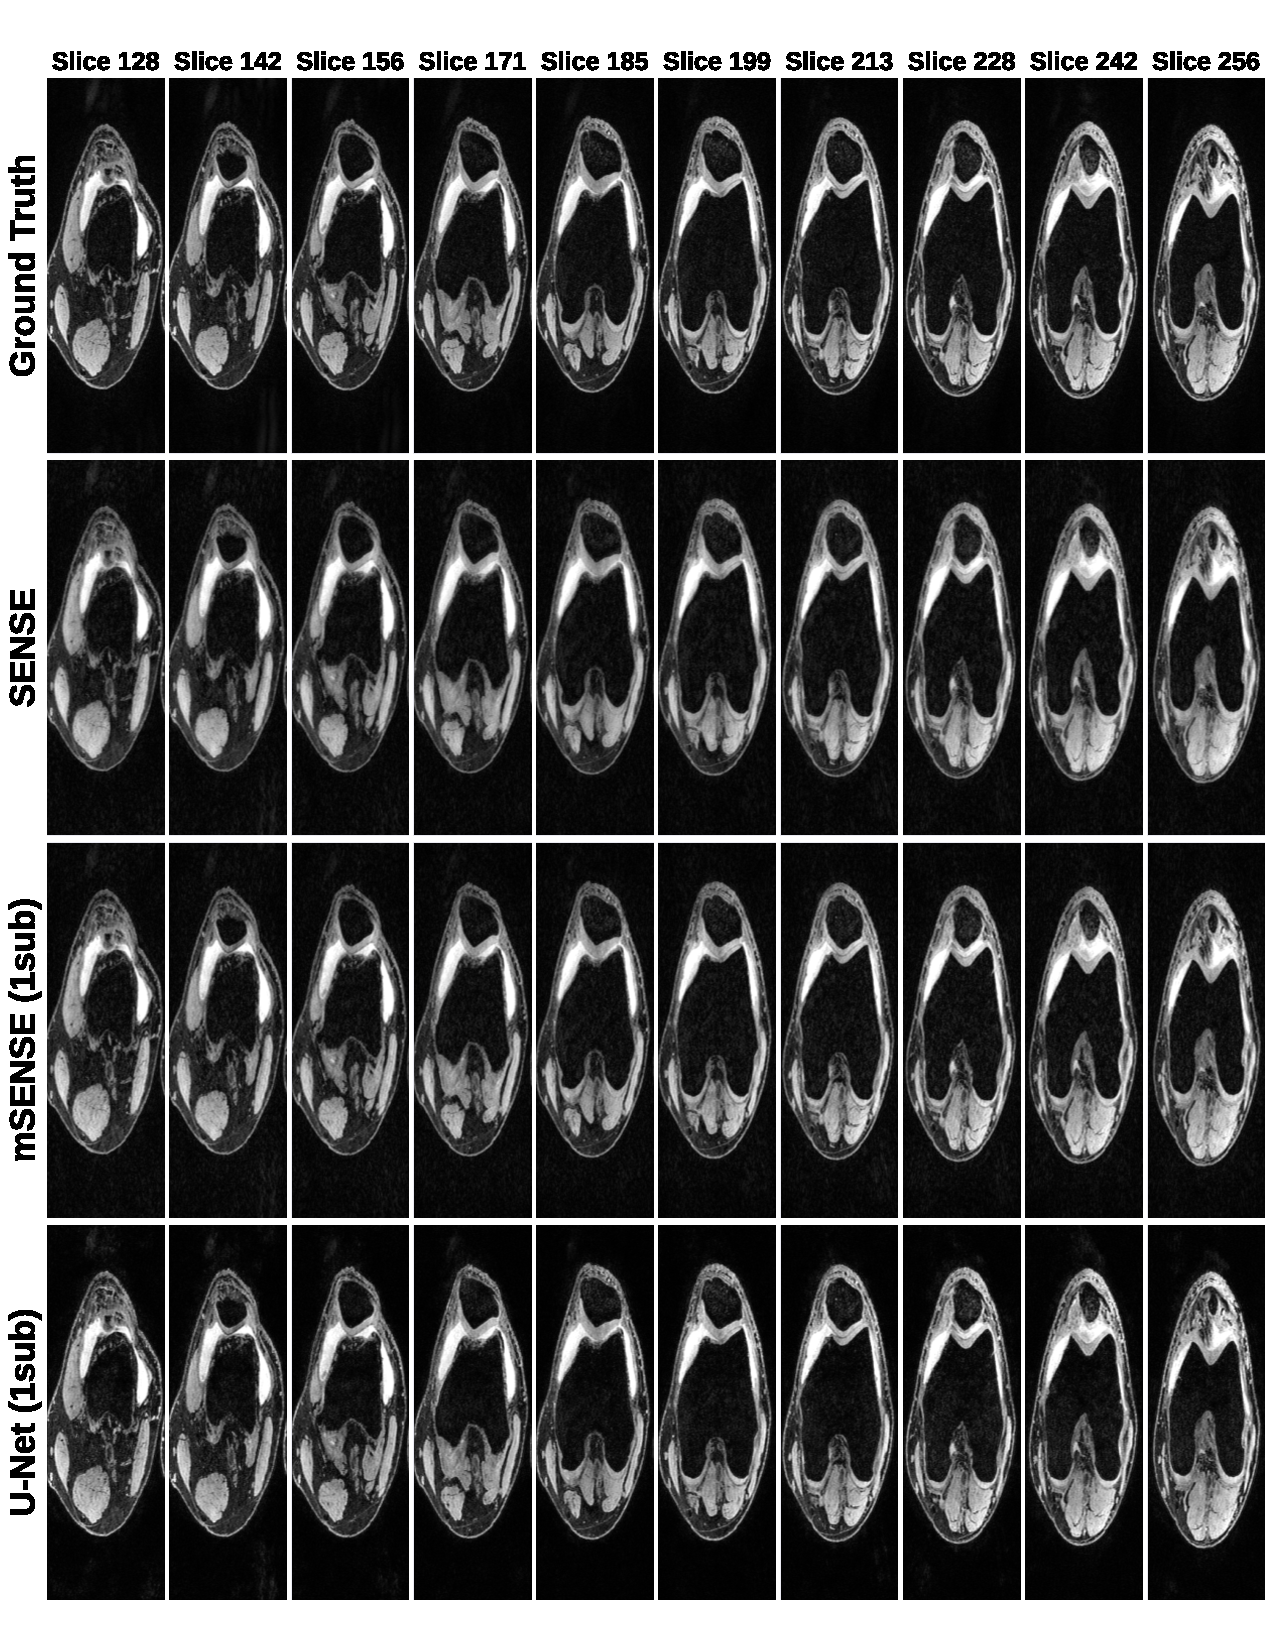
\includegraphics[width=0.9\linewidth]{figures/sample-mri-echo1.pdf}
    \vspace{-1em}
    \caption{Sample reconstructions at 2x acceleration for the first echo in the SKM-TEA dataset using SENSE, Monarch-SENSE (mSENSE), and U-Net. Both mSENSE and U-Net are trained with 1 training scan. SENSE is an untrained method.}
    \label{fig:mri-data-limited-echo1}
\end{figure}

\begin{figure}
    \centering
    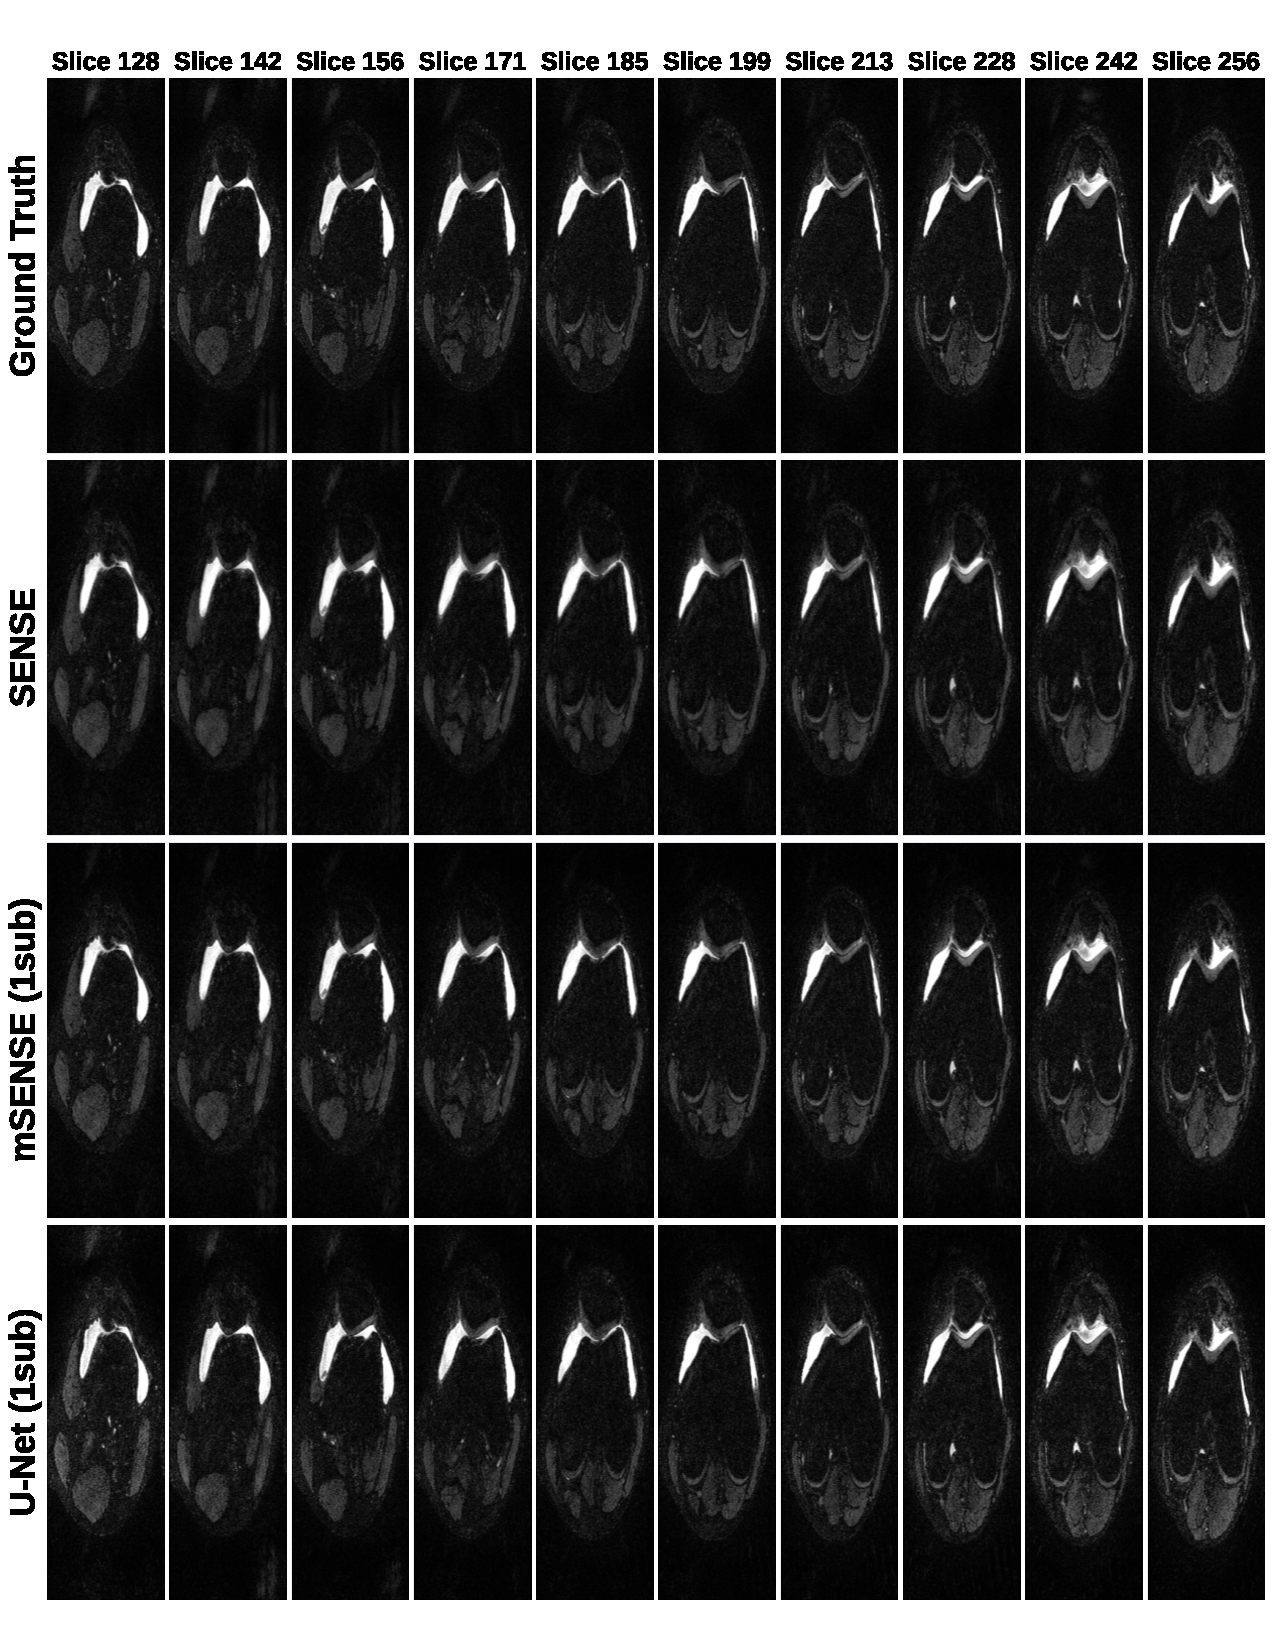
\includegraphics[width=6in]{figures/sample-mri-echo2.pdf}
    \vspace{-1em}
    \caption{Sample reconstructions at 2x acceleration for the second echo in the SKM-TEA dataset using SENSE, Monarch SENSE (mSENSE), and U-Net. Both mSENSE and U-Net are trained with 1 training scan. SENSE is an untrained method.}
    \label{fig:mri-data-limited-echo2}
\end{figure}









\end{document}
